\chapter{Differential Forms, Stokes' Theorem, and Calculus on Manifolds}
\label{ch:forms-stokes}
\chaptermark{Forms}

\section{Parametrized Curves and Line Integrals}
Integration can accumulate mass along a wire or work along a path. The same
geometric curve supports both questions, but they require different integrands:
mass uses length, while work records direction. We start with these familiar
quantities before introducing the objects that unify their boundary formulas.

\paragraph{Recall and choose a parametrization.}
Chapter~8 introduced plane curves in ``\nameref{sec:elementary-curves-polar}'';
\cref{def:curve-velocity} identified coordinatewise velocity with the
Fr\'echet derivative. Recalling those choices, now also using vector notation,
\[
\begin{array}{ll}
\text{segment from }p\text{ to }q & \gamma(t)=(1-t)p+tq,\quad 0\leq t\leq1,\\
\text{graph }y=f(x) & \gamma(t)=(t,f(t)),\quad t\text{ in the graph's interval},\\
\text{circle of radius }R>0 & \gamma(t)=(R\cos t,R\sin t),\quad0\leq t\leq2\pi,\\
\text{ellipse, }a,b>0 & \gamma(t)=(a\cos t,b\sin t),\quad0\leq t\leq2\pi,\\
\text{polar curve }r=\rho(\theta) &
\gamma(\theta)=(\rho(\theta)\cos\theta,\rho(\theta)\sin\theta).
\end{array}
\]
For the polar curve choose the desired angular interval and $\rho\geq0$.
Start by identifying the set and the intended traversal. Choose one scalar
parameter, express every coordinate in it, and select an interval covering
exactly the desired portion. Check endpoints, orientation, and multiplicity;
then differentiate to obtain velocity and speed. The geometric image does
not determine the traversal: speed, direction, and the number of passes
can all change while the image stays fixed.

By \cref{prop:curve-chain-rule},
\[
(f\circ\gamma)'(t)=Df(\gamma(t))\gamma'(t).
\]
It transports tangent velocities through maps. For scalar $f$ it pairs the
derivative covector with velocity; this will explain work for gradient
fields, the fundamental theorem for line integrals, and curve pullback.

\subsection{A curve is a traversal, not just a set}
The maps $t\mapsto(\cos t,\sin t)$ on $[0,2\pi]$ and
$t\mapsto(\cos2t,\sin2t)$ on the same interval have the same image,
but the second traverses it twice. Integrals can distinguish these maps.
The velocity $\gamma'(t)$ is a tangent vector; its norm is speed.
For a short time $\Delta t$, the displacement is approximately
$\gamma'(t)\Delta t$ and the distance traveled is approximately
$\|\gamma'(t)\|\Delta t$. This suggests length as accumulated speed.

For a scalar density $f$, multiply each small length by $f$ to obtain
a scalar line integral. For a force field $F$, multiply displacement by
the component of force in its direction: $F\cdot\gamma'\Delta t$.
This gives work. These two constructions use different information,
although both are computed by a one-variable integral.
\begin{figure}[htbp]
\centering
\begin{tikzpicture}[font=\small,>=Stealth]

\draw[gray,thick] (-1,-.3) .. controls (-.6,0) and (-.3,0) .. (0,0)
 .. controls (1,0) and (2,0) .. (3.3,.7);
\fill (0,0) circle (2pt) node[below left] {$\gamma(t)$};
\draw[->,very thick,blue] (0,0)--(3,0) node[below] {$\gamma'(t)\Delta t$};
\draw[->,very thick,red!70!black] (0,0)--(2,2) node[above] {$F(\gamma(t))$};
\draw[dashed] (2,2)--(2,0);
\draw[->,thick,red!70!black] (0,.13)--(2,.13) node[midway,above] {$F_{\parallel}\tau$};
\draw (1.8,0)--(1.8,.2)--(2,.2);
\node[align=left,text width=6cm,anchor=west] at (4,1) {
$\tau=\gamma'/\|\gamma'\|$, $F_{\parallel}=F\cdot\tau$ is scalar.\\[3pt]
Only the tangential component contributes:\\[3pt]
$F\cdot\gamma'\Delta t=F_{\parallel}\|\gamma'\|\Delta t$.\\[5pt]
Length uses $\|\gamma'\|\Delta t$,\\
independent of the force or its sign.};

\end{tikzpicture}
\caption{The dot product extracts the force component along displacement. The blue vector follows the velocity $\gamma'(t)$ and approximates the actual short displacement along the curve.}
\label{fig:work-projection}
\end{figure}

\begin{definition}[Parametrized curve and velocity]
For the recalled parametrized curves, our integration convention is a
map $\gamma:[a,b]\to\R^n$ of class $C^1$, with
continuous derivative, using one-sided derivatives at endpoints.
Its velocity at time $t$ is $\gamma'(t)$, and it is \textbf{regular}
if this vector is never zero. Its orientation is the direction of
increasing parameter. Its image is the set $\gamma([a,b])$, which
does not record the speed or multiplicity of traversal.
\end{definition}
For $\gamma(t)=(t,t^2)$ the velocity is $(1,2t)$ and the speed
$\sqrt{1+4t^2}$ varies with time. A tangent vector is a displacement
direction; speed is a nonnegative scalar.
\begin{definition}[Smooth-curve length]
We define the length of a $C^1$ curve by
\[
\ell(\gamma)=\int_a^b\|\gamma'(t)\|\,\dd t.
\]
For continuous piecewise $C^1$ curves, add the lengths of the finitely
many smooth pieces. Refining that subdivision does not change the sum,
by additivity of the one-variable integral. No equivalence with a
polygonal-supremum definition is assumed here.
\end{definition}
To integrate a scalar function along the curve, the small length is
weighted by the scalar value at the visited point.
For the fixed curve $\gamma:[a,b]\to\R^n$, the field types are
$f:\gamma([a,b])\to\R$ and $F:\gamma([a,b])\to\R^n$.
Assume these fields are continuous. The actual integrands on the parameter interval are the scalar functions
\[
g(t)=f(\gamma(t))\|\gamma'(t)\|,\qquad
h(t)=F(\gamma(t))\cdot\gamma'(t).
\]
Both are continuous on each smooth piece, so Chapter~9 supplies their
integrals. Thus the following definitions are the ordinary integrals
\[
\int_a^b g(t)\,\dd t,
\qquad
\int_a^b h(t)\,\dd t.
\]
The curve lies in $\R^n$ but the integration
domain is one-dimensional. Work is scalar because the dot product is taken
\emph{before} integration; it differs from the componentwise vector
integral
\[
\int_a^bF(\gamma(t))\,\dd t.
\]

\begin{definition}[Scalar line integral]
For continuous $f$ along the image of $\gamma$, set
\[
\int_\gamma f\,\dd s
=\int_a^b f(\gamma(t))\|\gamma'(t)\|\,\dd t.
\]
Taking $f=1$ recovers length. Negative values of $f$ contribute negatively.
\end{definition}
\paragraph{Arc length is not a coordinate differential.}
Coordinate covectors are linear: $\dd x(-v)=-\dd x(v)$. Length instead
satisfies $\|-v\|=\|v\|$. Thus the parametrization shorthand
$\dd s=\|\gamma'(t)\|\,\dd t$ records a speed factor in an ordinary
integral, not evaluation of a linear $1$-form analogous to $\dd x$.
This explains why scalar arc-length integrals are independent of orientation,
whereas work and $1$-form integrals change sign under reversal.
For the counterclockwise unit circle on $[0,2\pi]$,
\[
\int_\gamma\dd x=\int_0^{2\pi}(-\sin t)\,\dd t=0,
\qquad \int_\gamma\dd s=\int_0^{2\pi}1\,\dd t=2\pi.
\]
Here the first integral means accumulating the coordinate covector on
velocity; the work-integral definition below includes this case.

Work instead pairs a vector field with the directed displacement.
\begin{definition}[Work integral]
For a continuous vector field $F$ along the image, set
\[
\int_\gamma F\cdot\dd r
=\int_a^b F(\gamma(t))\cdot\gamma'(t)\,\dd t.
\]
Both kinds of line integral extend to piecewise $C^1$ curves by finite
addition over their smooth pieces.
\end{definition}
\begin{proposition}[Reparametrization and reversal]
\label{prop:curve-reparametrization}
Let $h:[c,d]\to[a,b]$ be a $C^1$ diffeomorphism and set
$\widetilde\gamma=\gamma\circ h$. The scalar line integral and length are
unchanged. The work integral is unchanged if $h$ is increasing and changes
sign if $h$ is decreasing.
\end{proposition}
\begin{proof}
The chain rule gives $\widetilde\gamma'=\gamma'(h)h'$, and hence
$\|\widetilde\gamma'\|=\|\gamma'(h)\||h'|$. If $h$ is increasing,
substitution in Chapter~\ref{ch:riemann} gives both assertions. If it is
decreasing, substitution with $h'$ changes the limits from $b$ to $a$.
For work this contributes a minus sign. For the scalar integral,
$|h'|=-h'$ contributes a second minus sign, cancelling the first.
\end{proof}
Thus
\[
\int_C f\,\dd s
\]
 is independent of orientation, but it need not
be positive: if $f=-1$ on a nonconstant curve, it equals minus the length.
In contrast,

\[
\int_C F\cdot\dd r
\]
 is signed. The notation $C$ presupposes a specified
traversal up to these reparametrizations: tracing a curve twice generally
doubles its integral and is not a diffeomorphic reparametrization.

\begin{figure}[htbp]
\centering
\begin{tikzpicture}[font=\small,>=Stealth]

\foreach \x in {0,6}{\begin{scope}[xshift=\x cm]
\draw[thick,blue] (0,0) .. controls (1,1.4) and (2,1.4) .. (3,0);
\fill (0,0) circle (1.5pt);\fill (3,0) circle (1.5pt);
\end{scope}}
\draw[->,very thick,red!70!black] (1.1,1.03)--(1.9,1.03);
\draw[<-,very thick,red!70!black] (7.1,1.03)--(7.9,1.03);
\node at (1.5,-.5) {$\gamma$};\node at (7.5,-.5) {$\widetilde\gamma$};
\node[align=center] at (4.5,-1.3) {$ds$ unchanged: same speed factor\\$dr$ reversed: opposite displacement};

\end{tikzpicture}
\caption{The same arc with opposite traversals. Scalar arc-length integrals are unchanged; work and $1$-form integrals change sign.}
\label{fig:curve-reversal}
\end{figure}

\begin{example}[Changing speed and reversing direction]
Let $\gamma(t)=(t,t^2)$ for $0\leq t\leq1$ and

\[
h(s)=(s+s^2)/2
\]
 on $[0,1]$. Then
\[
h'(s)=(1+2s)/2>0,
\]

so $h$ is an increasing diffeomorphism with the same endpoint values.
The new velocity is $(h'(s),2h(s)h'(s))$; the traversal speeds differ,
but substitution shows both lengths equal

\[
\int_0^1\sqrt{1+4t^2}\,\dd t.
\]

For $F=(1,0)$, both work integrals are $1$: in the new parameter
the integral is
\[
\int_0^1h'(s)\,\dd s=h(1)-h(0).
\]

Using $h(s)=1-s$ instead reverses direction and gives work $-1$.
The scalar integral of $f=-1$ stays the same negative length.
\end{example}
For a planar curve $\gamma(t)=(x(t),y(t))$, the notation means
\[
\int_\gamma P\,\dd x+Q\,\dd y
=\int_a^b[P(x(t),y(t))x'(t)+Q(x(t),y(t))y'(t)]\,\dd t.
\]
As previewed after \cref{prop:curve-chain-rule}, along the parametrization
$\dd x$ becomes $x'(t)\,\dd t$ and $\dd y$ becomes $y'(t)\,\dd t$.
These are evaluations of the coordinate covectors on velocity; later
we formalize the resulting parameter-line covectors as pullbacks.
These differential factors are not the Chapter~12 area notation $\dd(x,y)$.

\begin{example}[One running circulation]
For $F(x,y)=(-y,x)$ and the counterclockwise unit circle
$\gamma(t)=(\cos t,\sin t)$, $0\leq t\leq2\pi$, the velocity is $F(\gamma(t))$.
Thus its length and circulation are both $2\pi$. Reversal keeps the length
and negates the circulation. The expression $x\,\dd y-y\,\dd x$ will
reappear as a differential form later in this chapter.
\end{example}

\begin{theorem}[Fundamental theorem for line integrals]
\label{thm:line-ftc}
If $f$ is $C^1$ near a piecewise $C^1$ curve $\gamma$, then
\[
\int_\gamma\nabla f\cdot\dd r=f(\gamma(b))-f(\gamma(a)).
\]
\end{theorem}
\begin{proof}
On each smooth piece the chain rule gives
$(f\circ\gamma)'=Df(\gamma)\gamma'=\nabla f(\gamma)\cdot\gamma'$.
Integrate by the one-variable FTC. Intermediate endpoint values cancel
when the pieces are added.
\end{proof}
Reparametrization invariance compares the same traversal at different
speeds or coordinates. Path independence compares genuinely different
curves with the same endpoints. The latter requires a special hypothesis:
the theorem shows that work for $F=\nabla f$ depends only on endpoints,
so any two such curves have the same work.

This is our first boundary/interior formula: integrating a derivative along
the interior leaves only the oriented endpoint values.

\begin{exercise}
Integrate $F=(2x,y)$ along the segment from $(0,0)$ to $(1,2)$, directly
and using a potential. Compute
\[
\int_C y\,\dd s
\]
 as well and explain how
the two answers change under reversal.
\end{exercise}


\subsection{Computing line integrals}
\begin{center}
\fbox{\parbox{.88\linewidth}{\textbf{Working rule.} Write $\gamma(t)$,
differentiate to obtain $\gamma'(t)$, and substitute along the curve.
For scalar density integrate $f(\gamma(t))\|\gamma'(t)\|$; for work
integrate $F(\gamma(t))\cdot\gamma'(t)$. The curve can live in $\R^n$,
but the parameter is one-dimensional. For work the dot product is taken
\emph{before} the ordinary scalar integral.}}
\end{center}
\begin{example}[Mass of a quarter-circle wire]
Let $R>0$ and $\gamma(t)=(R\cos t,R\sin t)$ for
\[
0\leq t\leq\pi/2.
\]

For density $\rho(x,y)=x+y$, we have
$\gamma'=(-R\sin t,R\cos t)$ and $\|\gamma'\|=R$. Thus the mass is
\[
\int_\gamma\rho\,\dd s=R^2\int_0^{\pi/2}(\cos t+\sin t)\,\dd t=2R^2.
\]
The density is nonnegative on this wire; reversing traversal leaves its
mass unchanged.
\end{example}
\begin{example}[Work along a segment]
For $\gamma(t)=(t,2t)$, $0\leq t\leq1$, and $F(x,y)=(y,x)$,
\[
F(\gamma(t))=(2t,t),\quad \gamma'(t)=(1,2),\quad
F(\gamma(t))\cdot\gamma'(t)=4t.
\]
Consequently
\[
\int_\gamma F\cdot\dd r=\int_0^1 4t\,\dd t=2.
\]

The reverse traversal has work $-2$.
\end{example}
\begin{example}[A helix]
For $R>0$, $c>0$, let $\gamma(t)=(R\cos t,R\sin t,ct)$,
$0\leq t\leq2\pi$. Its derivative is $(-R\sin t,R\cos t,c)$, so
\[
\operatorname{length}(\gamma)=2\pi\sqrt{R^2+c^2},\qquad
\int_\gamma z\,\dd s=\int_0^{2\pi}ct\sqrt{R^2+c^2}\,\dd t
=2\pi^2c\sqrt{R^2+c^2}.
\]
\begin{center}
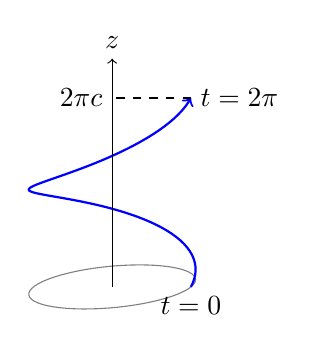
\begin{tikzpicture}[x={(1cm,0cm)},y={(.35cm,.28cm)},z={(0cm,1cm)}]
\draw[gray] plot[domain=0:360,samples=60] ({cos(\x)},{sin(\x)},0);
\draw[blue,thick,->] plot[domain=0:360,samples=80] ({cos(\x)},{sin(\x)},{\x/150});
\draw[->] (0,0,0)--(0,0,2.9) node[above] {$z$};
\draw[dashed] (1,0,2.4)--(0,0,2.4) node[left] {$2\pi c$};
\node[below] at (1,0,0) {$t=0$};\node[right] at (1,0,2.4) {$t=2\pi$};
\end{tikzpicture}
\end{center}
The arrow shows one traversal: one turn around the axis and rise $2\pi c$.
\end{example}

\section{Green's Theorem in the Plane}
The next formula turns circulation around a planar boundary into accumulated
local rotation. We first prove it for a precise elementary class of regions.


Integrating a vertical derivative first subtracts its lower boundary value
from its upper value. Positive boundary traversal runs rightward on the
lower edge and leftward on the upper edge, explaining the minus sign in
the $P$ term. The horizontal calculation explains the $Q$ term. After
subdivision, a shared edge is traversed in opposite directions by its two
adjacent pieces, leaving only the outside boundary.
\begin{theorem}[Green for elementary planar regions]
\label{thm:green-elementary}
Suppose $D$ has both a vertical and a horizontal description
\[
\begin{split}
D&=\{(x,y):a\leq x\leq b,\ \alpha(x)\leq y\leq\beta(x)\},\\
D&=\{(x,y):c\leq y\leq d,\ \lambda(y)\leq x\leq\mu(y)\},
\end{split}
\]
where the four bounding functions are continuous and piecewise $C^1$,
with strict lower/upper inequalities in the interiors of their intervals.
Give its piecewise $C^1$ boundary the positive direction, with the region
on the left. If $P,Q$ are $C^1$ on a neighborhood of $D$, then
\[
\int_{\partial D}P\,\dd x+Q\,\dd y
=\int_D(Q_x-P_y)\,\dd(x,y).
\]
The formula also holds for a finite union of such regions with disjoint
interiors and shared boundary arcs that cancel in opposite directions.
\end{theorem}
\begin{center}
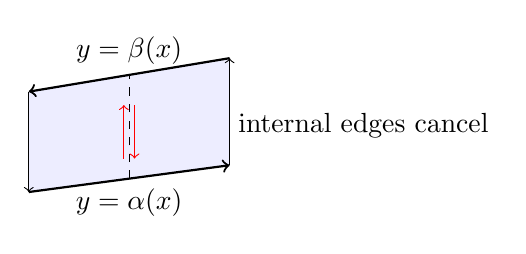
\begin{tikzpicture}[scale=.85]
\fill[blue!7] (0,.3)--(3,.7)--(3,2.3)--(0,1.8)--cycle;
\draw[->,thick] (0,.3)--(3,.7) node[midway,below] {$y=\alpha(x)$};
\draw[->,thick] (3,2.3)--(0,1.8) node[midway,above] {$y=\beta(x)$};
\draw[->] (3,.7)--(3,2.3); \draw[->] (0,1.8)--(0,.3);
\draw[dashed] (1.5,.5)--(1.5,2.05);
\draw[->,red] (1.42,.8)--(1.42,1.6);
\draw[->,red] (1.58,1.6)--(1.58,.8);
\node at (5,1.3) {internal edges cancel};
\end{tikzpicture}
\end{center}
\begin{proof}
Integrate $P_y$ vertically and $Q_x$ horizontally; the FTC
produces exactly the upper/lower and right/left boundary contributions.
By \cref{thm:simple-planar-region} and the FTC,
\[
-\int_D P_y=\int_a^b\bigl(P(x,\alpha(x))-P(x,\beta(x))\bigr)\,\dd x.
\]
The lower boundary goes left to right and the upper one right to left;
vertical boundary segments contribute nothing to $P\,\dd x$. This is
therefore
\[
\int_{\partial D}P\,\dd x.
\]
 Similarly,
\[
\int_D Q_x=\int_c^d\bigl(Q(\mu(y),y)-Q(\lambda(y),y)\bigr)\,\dd y
=\int_{\partial D}Q\,\dd y.
\]
The right boundary goes upward and the left downward. Add the identities.
For a finite decomposition, each $C^1$ arc on a compact interval has
bounded derivative, hence is Lipschitz by the mean-value estimate.
Its image is Jordan-null by \cref{lem:lipschitz-box-face} (a one-dimensional
face mapped into the plane). A piecewise $C^1$ arc is a finite union of
these null images. Overlaps of the regions lie in these boundary arcs,
so area integrals add by \cref{prop:jordan-null-additivity}. Each shared arc is
traversed twice in opposite directions, so its line integrals cancel.
\end{proof}
Rectangles and triangles belong to this class. The theorem does not assert
a decomposition for every conceivable piecewise smooth boundary. Later
manifold Stokes will supply the global smooth-boundary result.

\begin{example}[Area from circulation]
For
\[
P=-y/2,
\]

\[
Q=x/2,
\]
 one has $Q_x-P_y=1$. Thus for these regions
\[
\operatorname{area}(D)=\frac12\int_{\partial D}(x\,\dd y-y\,\dd x).
\]
On the triangle with vertices $(0,0),(1,0),(0,1)$, the two coordinate
edges contribute zero. On $(x,y)=(1-t,t)$, $0\leq t\leq1$, the integrand
is $\dd t$, yielding area
\[
1/2.
\]
 Internal-edge cancellation is already
a concrete model of the later passage from local formulas to a global one.
\end{example}
\begin{exercise}
Verify Green for $P=xy$, $Q=x^2$ on the unit square by computing all four
edge integrals. Then split the square along its diagonal and identify the
two cancelling contributions.
\end{exercise}

\section{Parametrized Surfaces and Surface Integrals}
A surface needs two independent tangent directions. A parametrization
turns a small parameter rectangle into an approximately planar parallelogram;
its area factor is the two-dimensional counterpart of $\|\gamma'\|$.

\begin{definition}[Cross product]
For $a,b\in\R^3$, define
\[
a\times b=(a_2b_3-a_3b_2,\ a_3b_1-a_1b_3,\ a_1b_2-a_2b_1).
\]
\end{definition}
\begin{proposition}[Cross-product identities]\label{prop:cross-product-identities}
The cross product is linear in each slot, and
\[
a\times b=-b\times a,\qquad a\times a=0.
\]
For $a,b,c\in\R^3$,
\[
(a\times b)\cdot c=\det(a,b,c),\qquad
\|a\times b\|^2=\|a\|^2\|b\|^2-(a\cdot b)^2.
\]
The cross product is orthogonal to $a,b$ (meaning that its Euclidean dot
product with each is zero). It is nonzero exactly when $a,b$ are independent,
and its norm is their parallelogram area.
\end{proposition}
\begin{proof}
Each coordinate $a_i b_j-a_j b_i$ is linear separately in $a$ and $b$.
For example, the first coordinate of $(a+a')\times b$ is
\[
(a_2+a'_2)b_3-(a_3+a'_3)b_2
=(a_2b_3-a_3b_2)+(a'_2b_3-a'_3b_2).
\]
The other two coordinates and scalar multiplication give
$(a+a')\times b=a\times b+a'\times b$ and
$(ta)\times b=t(a\times b)$; the same calculation applies to the second
slot. Interchanging $a,b$ negates every coordinate; equal inputs give zero.
The dot product expands as
$(a_2b_3-a_3b_2)c_1+(a_3b_1-a_1b_3)c_2+(a_1b_2-a_2b_1)c_3$,
the determinant expansion in the third column. Taking $c=a$ or $c=b$
gives zero by alternation. For the squared norm, expansion gives
\[
\sum_{i<j}(a_ib_j-a_jb_i)^2
=\sum_{i\ne j}a_i^2b_j^2-2\sum_{i<j}a_ia_jb_ib_j
=\|a\|^2\|b\|^2-(a\cdot b)^2.
\]
If $a\ne0$, write $b=ta+h$ with
\[
t=(a\cdot b)/\|a\|^2
\]
 and
$a\cdot h=0$. Substitution in the last identity gives
$\|a\times b\|^2=\|a\|^2\|h\|^2$. It vanishes exactly when $b$ is
a multiple of $a$; otherwise $\|a\|$ and $\|h\|$ are the base and
perpendicular height. If $a=0$, both the cross product and the area are zero,
and the pair is dependent.
\end{proof}
\begin{definition}[Regular surface patch and its orientation]
Let $D\subset\R^2$ be a compact Jordan region equal to the closure of its
interior. A regular $C^1$ surface patch is a $C^1$ map $\sigma$ on an open
neighborhood of $D$, injective on $D$, with independent derivatives
$\sigma_u,\sigma_v$ throughout $D$. Its tangent plane at $\sigma(u,v)$ is the
span of these vectors, translated to that point. The parameter order $(u,v)$
chooses the unit normal
\[
n=\frac{\sigma_u\times\sigma_v}{\|\sigma_u\times\sigma_v\|}.
\]
The opposite normal gives the reverse orientation.
\end{definition}

\subsection{A small parameter rectangle becomes a tangent parallelogram}
At $(u,v)$ the two edge increments are approximately
$\sigma_u\Delta u$ and $\sigma_v\Delta v$. Their parallelogram has area
$\|\sigma_u\times\sigma_v\|\Delta u\Delta v$.
The scalar $\|\sigma_u\times\sigma_v\|$ measures area per unit parameter
area. The vector $\sigma_u\times\sigma_v$ contains the same magnitude
together with an oriented normal direction. Taking its norm loses precisely
the information that flux needs.

For a regular patch $\sigma:D\subseteq\R^2\to\R^3$,
$D\sigma(u,v):\R^2\to\R^3$ has a $3\times2$ matrix with columns
$\sigma_u,\sigma_v\in\R^3$; $\det D\sigma$ is not defined. Put $a_\sigma=\|\sigma_u\times\sigma_v\|>0$
and
\[
n=(\sigma_u\times\sigma_v)/a_\sigma.
\]
 The area factor $a_\sigma$ is
a scalar, $n$ a unit vector, and for $f:S\to\R$, $F:S\to\R^3$,
both $f(\sigma)a_\sigma$ and $(F(\sigma)\cdot n)a_\sigma$ are scalars on $D$.
In particular,
\[
(F(\sigma)\cdot n)a_\sigma
=F(\sigma)\cdot\left(\frac{\sigma_u\times\sigma_v}{a_\sigma}a_\sigma\right)
=F(\sigma)\cdot(\sigma_u\times\sigma_v).
\]
Here $\dd S$ denotes surface area and $\dd(u,v)$ parameter-plane area.
All these are double integrals: the ambient space $\R^3$ does not make
the parameter domain three-dimensional. Assume the fields $f,F$ are
continuous along the patch. Under the patch hypotheses,
the scalar coefficients are continuous on compact Jordan $D$, so their
integrals exist by Chapter~12.

\begin{figure}[htbp]
\centering
\begin{tikzpicture}[font=\small,>=Stealth]

\filldraw[fill=blue!8,draw=blue] (0,0) rectangle (1.8,1.3);
\draw[->] (0,-.2)--(1.8,-.2) node[midway,below] {$\Delta u$};
\draw[->] (-.2,0)--(-.2,1.3) node[midway,left] {$\Delta v$};
\node at (.9,2) {parameter rectangle};
\draw[->,thick] (2.1,.7)--(3,.7) node[midway,above] {$\sigma$};
\filldraw[fill=blue!8,draw=blue,thick] (3.3,0) .. controls (4,.4) and (4.7,.2) .. (5.3,.5)
 .. controls (5.2,1.1) and (5.6,1.4) .. (5.3,1.7)
 .. controls (4.7,1.4) and (4,1.8) .. (3.3,1.3)
 .. controls (3.5,.8) and (3.2,.5) .. (3.3,0);
\node at (4.3,2) {curved patch};
\draw[->,thick] (5.7,.7)--(6.6,.7);
\filldraw[fill=blue!8,draw=blue] (7,0)--(9,0)--(9.6,1.3)--(7.6,1.3)--cycle;
\draw[->,very thick] (7,0)--(9,0) node[midway,below] {$\sigma_u\Delta u$};
\draw[->,very thick] (7,0)--(7.6,1.3) node[pos=.65,right] {$\sigma_v\Delta v$};
\node at (8.3,2) {tangent parallelogram};
\node at (5,-1.25) {area to first order: $\|\sigma_u\times\sigma_v\|\Delta u\Delta v$};

\end{tikzpicture}
\caption{The derivative replaces a small curved patch by its tangent parallelogram. The cross-product norm gives the local scalar area factor.}
\label{fig:surface-area-mechanism}
\end{figure}

\begin{definition}[Area, scalar surface integral, and flux]
For $S=\sigma(D)$ and continuous $f,F$ along $S$, define
\[
\operatorname{area}(S)=\int_D\|\sigma_u\times\sigma_v\|\,\dd(u,v),
\qquad
\int_S f\,\dd S=\int_D f(\sigma)\|\sigma_u\times\sigma_v\|\,\dd(u,v),
\]
\[
\int_S F\cdot n\,\dd S=\int_D F(\sigma)\cdot(\sigma_u\times\sigma_v)\,\dd(u,v).
\]
These are classical smooth parametrized-surface integrals. We are not
constructing an independent general surface-measure theory.
\end{definition}

\begin{figure}[htbp]
\centering
\begin{tikzpicture}[font=\small,>=Stealth]

\filldraw[fill=blue!8,draw=blue] (-1,-.6)--(2,-.6)--(3,.4)--(0,.4)--cycle;
\fill (1,0) circle (2pt);
\draw[->,very thick,blue] (1,0)--(1,2.3) node[above] {$n$};
\draw[->,very thick,red!70!black] (1,0)--(3.2,1.6) node[right] {$F$};
\draw[dashed] (3.2,1.6)--(1,1.6);
\draw[->,thick,red!70!black] (.88,0)--(.88,1.6) node[left] {$(F\cdot n)n$};
\node[align=left,anchor=west] at (4,1) {$\displaystyle n=\dfrac{\sigma_u\times\sigma_v}{\|\sigma_u\times\sigma_v\|}$\\[8pt]
$F\cdot n\,dS$\\[3pt]$\quad=F\cdot(\sigma_u\times\sigma_v)\,du\,dv$};
\node[align=center] at (4,-1.3) {Swap $u,v$: the normal and flux reverse;\\the parallelogram area is unchanged.};

\end{tikzpicture}
\caption{Flux measures the normal component of the field. Tangential motion contributes no flux through the patch. The sketch uses a positively directed normal component.}
\label{fig:flux-normal}
\end{figure}

\begin{proposition}[Surface reparametrization]
Let $\widetilde\psi:U'\to U$ be a $C^1$ diffeomorphism between open
neighborhoods of $D'$ and $D$, with $\widetilde\psi(D')=D$, and put
$\psi=\widetilde\psi|_{D'}$. Then scalar surface integrals are unchanged. Flux is unchanged for a
positive determinant and changes sign for a negative determinant.
\end{proposition}
\begin{proof}
First $D'=\widetilde\psi^{-1}(D)$ is compact, and
\cref{lem:c1-jordan-null} applied to the inverse diffeomorphism makes it
Jordan measurable. A homeomorphism of neighborhoods preserves interiors
and closures, so $D'=\overline{(D')^\circ}$ as well. Thus it is an
admissible parameter region before change of variables is used.
Write $\psi(s,t)=(u(s,t),v(s,t))$. With $\sigma_u,\sigma_v$ evaluated
at $\psi(s,t)$, the chain rule gives
\[
(\sigma\circ\psi)_s=\sigma_u u_s+\sigma_v v_s,\qquad
(\sigma\circ\psi)_t=\sigma_u u_t+\sigma_v v_t.
\]
Expanding their cross product gives zero from the two equal-vector terms;
the remaining terms are $u_sv_t(\sigma_u\times\sigma_v)$ and
$v_su_t(\sigma_v\times\sigma_u)=-v_su_t(\sigma_u\times\sigma_v)$.
Their sum has coefficient $u_sv_t-v_su_t=\det D\psi$. This determinant
belongs to the $2\times2$ change of parameters; the original $3\times2$
surface derivative has no determinant. Thus
\[
(\sigma\circ\psi)_s\times(\sigma\circ\psi)_t
=(\det D\psi)(\sigma_u\times\sigma_v)\circ\psi.
\]
Taking norms produces $|\det D\psi|$ for scalar integrals; retaining the
vector produces $\det D\psi$ for flux. Apply \cref{cor:jordan-nonlinear-change} to obtain both assertions.
\end{proof}


At this stage these are integrals of a chosen parametrized patch,
invariant under the admissible reparametrizations just proved. Full
chart-independence for smooth surfaces follows later from manifold integration.

\subsection{Computing surface area and flux}
\begin{center}
\fbox{\parbox{.88\linewidth}{\textbf{Working rule.} Write $\sigma(u,v)$,
compute $\sigma_u,\sigma_v$, then $\sigma_u\times\sigma_v$.
For scalar surface integration use $f(\sigma)\|\sigma_u\times\sigma_v\|$;
for flux use $F(\sigma)\cdot(\sigma_u\times\sigma_v)$, and take the ordinary
double integral. Here $D\sigma$ is $3$ by $2$, so $\det D\sigma$ is undefined.}}
\end{center}
\begin{example}[A plane patch]
For $\sigma(u,v)=(u,v,u+2v)$ on $[0,1]^2$,
\[
\sigma_u=(1,0,1),\quad \sigma_v=(0,1,2),\quad
\sigma_u\times\sigma_v=(-1,-2,1).
\]
Thus
\[
\operatorname{area}(S)=\int_0^1\int_0^1\sqrt6\,\dd v\,\dd u=\sqrt6.
\]

\begin{center}
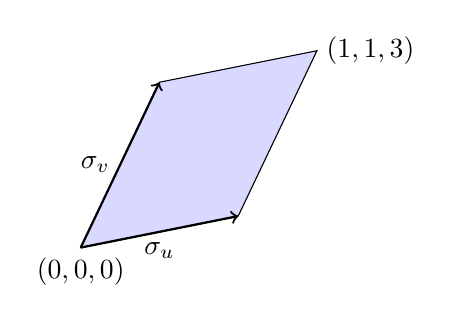
\begin{tikzpicture}[x={(2cm,-.4cm)},y={(1cm,.5cm)},z={(0cm,.8cm)}]
\filldraw[fill=blue!15] (0,0,0)--(1,0,1)--(1,1,3)--(0,1,2)--cycle;
\draw[->,thick] (0,0,0)--(1,0,1) node[midway,below] {$\sigma_u$};
\draw[->,thick] (0,0,0)--(0,1,2) node[midway,left] {$\sigma_v$};
\node[right] at (1,1,3) {$(1,1,3)$};
\node[below] at (0,0,0) {$(0,0,0)$};
\end{tikzpicture}
\end{center}
The unit parameter square becomes this parallelogram with area $\sqrt6$.
For the nonconstant scalar field $f(x,y,z)=z$, substitute $z=u+2v$ and
use the same unsigned area factor:
\begin{align*}
\int_S z\,\dd S
&=\sqrt6\int_0^1\int_0^1(u+2v)\,\dd v\,\dd u\\
&=\sqrt6\int_0^1[uv+v^2]_{v=0}^{v=1}\,\dd u
=\sqrt6\int_0^1(u+1)\,\dd u=\frac32\sqrt6.
\end{align*}
For $F=(0,0,z)$, the upward cross product instead gives
$F(\sigma)\cdot(\sigma_u\times\sigma_v)=u+2v$. Thus
\[
\int_S F\cdot n\,\dd S=\int_0^1\int_0^1(u+2v)\,\dd v\,\dd u
=\int_0^1(u+1)\,\dd u=\frac32.
\]
Area $\sqrt6$, scalar-weighted area
\[
\frac{3\sqrt6}{2},
\]
 and flux

\[
\frac32
\]
 are
three different integrals on the same surface. The scalar density weights
unsigned area; flux measures the field's oriented normal component.

\end{example}
\begin{example}[The side of a cylinder]
For $R,h>0$, parametrize the side by
\[
\sigma(\theta,z)=(R\cos\theta,R\sin\theta,z),\quad
0\leq\theta\leq2\pi,\quad0\leq z\leq h.
\]
Use two half-cylinder patches to avoid the repeated seam; their common
edges contribute zero parameter area. We obtain
\[
\sigma_\theta=(-R\sin\theta,R\cos\theta,0),\quad \sigma_z=(0,0,1),
\quad\sigma_\theta\times\sigma_z=(R\cos\theta,R\sin\theta,0).
\]
This points outward and has norm $R$, so the side area is
\[
\operatorname{area}(S)=\int_0^{2\pi}\int_0^h R\,\dd z\,\dd\theta
=\int_0^{2\pi}Rh\,\dd\theta=2\pi Rh.
\]
For $F(x,y,z)=(x,y,0)$, first take the dot product:
\[
F(\sigma)\cdot(\sigma_\theta\times\sigma_z)
=R^2\cos^2\theta+R^2\sin^2\theta=R^2.
\]
Hence the outward flux is
\[
\int_S F\cdot n\,\dd S=\int_0^{2\pi}\int_0^h R^2\,\dd z\,\dd\theta
=\int_0^{2\pi}R^2h\,\dd\theta=2\pi R^2h.
\]
The compact angular notation represents the sum over the two injective
half-cylinder patches already specified. Reversing orientation negates
flux and preserves area. Chapter~12 computed the solid's volume $\pi R^2h$;
here we integrate over its two-dimensional side, excluding the caps.
\end{example}

\begin{example}[A graph and a simple flux]
For $\sigma(u,v)=(u,v,h(u,v))$,
\[
\sigma_u=(1,0,h_u),\quad\sigma_v=(0,1,h_v),\quad
\sigma_u\times\sigma_v=(-h_u,-h_v,1).
\]
The upward area factor is $\sqrt{1+h_u^2+h_v^2}$.
The upward flux of $(0,0,1)$ is
\[
\int_D1=\operatorname{area}(D),
\]

although the graph's surface area is generally larger. Reversing orientation
negates the flux and leaves the scalar area unchanged.
\end{example}

\begin{exercise}
For $\sigma(u,v)=(u,v,u+2v)$ on $[0,1]^2$, use the computed area factor to find the scalar surface integral of $x^2$ and upward
flux of $F=(0,0,y^2)$. Explain the effect of interchanging the parameter order.
\end{exercise}

\begin{example}[Area and flux on a curved paraboloid]
Let $\sigma(u,v)=(u,v,u^2+v^2)$ for $u^2+v^2\leq1$.
The map is injective because its first two coordinates recover $(u,v)$;
its cross product $(-2u,-2v,1)$ never vanishes and points upward.
Thus the area is
\[
\int_0^{2\pi}\int_0^1\sqrt{1+4r^2}\,r\,\dd r\,\dd\theta
=\frac{\pi}{6}(5^{3/2}-1).
\]
Here substitution $s=1+4r^2$, $\dd s=8r\dd r$ evaluates the inner
integral. For $F=(0,0,z)$ the upward flux is instead
\[
\int_{u^2+v^2\leq1}(u^2+v^2)\,\dd(u,v)
=2\pi\int_0^1r^3\,\dd r=\frac\pi2.
\]
The normalizing factor cancels against the scalar area factor in the
flux formula. Reversing the surface orientation negates only the flux.
\end{example}
\section{Classical Stokes for a Parametrized Surface Patch}

A parameter-plane velocity $(u',v')$ becomes
$\sigma_u u'+\sigma_v v'$ on the surface. Taking its dot product with
$F(\sigma)$ gives $A u'+B v'$ with
$A=F(\sigma)\cdot\sigma_u$ and $B=F(\sigma)\cdot\sigma_v$.
These coefficients are forced by the work integrand. Differentiating them
produces two kinds of terms: derivatives of $F$, through the chain rule,
and second derivatives of $\sigma$. In $B_u-A_v$ the latter cancel
because $\sigma_{vu}=\sigma_{uv}$. The surviving force-field derivatives
combine into the curl. This is the plan behind the component calculation.

\Needspace{9\baselineskip}
All four classical integrals have real outputs:
\begin{center}
\begin{tabular}{lll}
Integral & Field input & Output\\\hline
Scalar line integral & scalar & real number\\
Work & vector & real number\\
Scalar surface integral & scalar & real number\\
Flux & vector & real number
\end{tabular}
\end{center}
The parameter integrand is scalar in every case, unlike componentwise
vector integration, whose output is a vector.
\begin{figure}[htbp]
\centering
\begin{tikzpicture}[font=\small,>=Stealth]

\node (D) at (0,0) {$D\subset\R^2$};\node (S) at (6,0) {$S=\sigma(D)$};
\node (dD) at (0,1.5) {$\partial D$};\node (dS) at (6,1.5) {$\partial S$};
\draw[->,thick] (D)--(S) node[midway,above] {$\sigma$};
\draw[->,thick] (dD)--(dS) node[midway,above] {$\sigma|_{\partial D}$};
\draw[->] (dD)--(D);\draw[->] (dS)--(S);
\node[align=center] at (0,-1.1) {$A\,du+B\,dv$ on $\partial D$\\$B_u-A_v$ in $D$};
\node[align=center] at (6,-1.1) {work on $\partial S$\\curl flux through $S$};
\node at (3,-2.3) {$B_u-A_v=(\nabla\times F)(\sigma)\cdot(\sigma_u\times\sigma_v)$};

\end{tikzpicture}
\caption{Patch Stokes is Green\textquotesingle s theorem in parameters. The same parametrization transfers both the oriented boundary and its interior integrand.}
\label{fig:patch-stokes-mechanism}
\end{figure}

\begin{theorem}[Parametrized-patch Stokes theorem]
\label{thm:classical-patch-stokes}
Let $D$ satisfy \cref{thm:green-elementary}, let $\sigma$ be a regular $C^2$
patch on $D$, and let $F=(F_1,F_2,F_3)$ be $C^1$ near $S=\sigma(D)$.
Orient $S$ by $\sigma_u\times\sigma_v$, and traverse its boundary by the image
of the positive boundary of $D$. Here $\partial S$ means the patch
boundary $\sigma(\partial D)$, not the ambient topological boundary in $\R^3$. Then
\[
\int_{\partial S}F\cdot\dd r=\int_S(\nabla\times F)\cdot n\,\dd S,
\]
where $\nabla\times F=(\partial_yF_3-\partial_zF_2,
\partial_zF_1-\partial_xF_3,\partial_xF_2-\partial_yF_1)$.
\end{theorem}

\begin{proof}
Transport boundary work to the parameter plane, differentiate there,
and identify the interior integrand before applying Green. Put
$A=F(\sigma)\cdot\sigma_u$ and $B=F(\sigma)\cdot\sigma_v$.
The open set where $\sigma$ is defined and takes values in the domain of
$F$ contains $D$. On it $F\circ\sigma$ is $C^1$ and the first derivatives
of $\sigma$ are $C^1$, so $A,B$ are $C^1$ on an open neighborhood of $D$.
For each boundary piece $c(t)=(u(t),v(t))$, the chain rule gives
\[
(\sigma\circ c)'=\sigma_u(c)u'+\sigma_v(c)v',\qquad
F(\sigma(c))\cdot(\sigma\circ c)'=A(c)u'+B(c)v'.
\]
Integrating and adding boundary pieces yields

\[
\int_{\partial S}F\cdot\dd r=\int_{\partial D}A\,\dd u+B\,\dd v.
\]

The product and chain rules next give
\[
\begin{aligned}
B_u&=DF(\sigma)[\sigma_u]\cdot\sigma_v+F(\sigma)\cdot\sigma_{vu},\\
A_v&=DF(\sigma)[\sigma_v]\cdot\sigma_u+F(\sigma)\cdot\sigma_{uv}.
\end{aligned}
\]
Since $\sigma$ is $C^2$, its mixed derivatives agree and the last terms
cancel. Write $a=\sigma_u$, $b=\sigma_v$. The remaining expression, with
derivatives evaluated at $\sigma$, is
\[
\begin{split}
B_u-A_v
&=\sum_{i,j}(\partial_jF_i)(a_jb_i-b_ja_i)\\
&=(\partial_2F_3-\partial_3F_2)(a_2b_3-a_3b_2)\\
&\quad+(\partial_3F_1-\partial_1F_3)(a_3b_1-a_1b_3)\\
&\quad+(\partial_1F_2-\partial_2F_1)(a_1b_2-a_2b_1)\\
&=(\nabla\times F)(\sigma)\cdot(\sigma_u\times\sigma_v).
\end{split}
\]
Green gives the desired surface integral. Our boundary orientation is
precisely the one induced by the ordered tangent pair; reversing it and the
surface orientation negates both sides.
\end{proof}
This proves Stokes for one patch. An arbitrary compact oriented surface
may require several charts, and proving the global statement is the purpose
of the manifold machinery below.

\begin{example}[Stokes on a tilted patch]
Take $\sigma(u,v)=(u,v,u+v)$ on the unit square and

\[
F=(-y/2,x/2,0).
\]
 Its curl is $(0,0,1)$, so the flux is $1$.
Boundary work pulls back to
\[
(-v\,\dd u+u\,\dd v)/2;
\]
 the bottom and
left edges contribute zero and the other two contribute
\[
1/2
\]
 each.
\end{example}

\begin{proposition}[Divergence on a box]
For a $C^1$ vector field near a box $Q\subset\R^3$,

\[
\int_Q\operatorname{div}F=\int_{\partial Q}F\cdot n\,\dd S,
\]

where the right side is the sum of the outward fluxes across its six faces
and $\operatorname{div}F=\partial_xF_1+\partial_yF_2+\partial_zF_3$.
\end{proposition}
\begin{proof}
Integrate each $\partial_jF_j$ first in the $j$th coordinate by FTC and
then in the other two by Fubini. The endpoint difference is exactly the
flux through the positive and negative $j$-faces. Add the three identities.
\end{proof}
The curved-boundary divergence theorem will follow from general Stokes.

\section{Beyond One Parametrization: Why Manifolds?}
\label{sec:manifold-preview}
A single parametrization describes only one coordinate region. A sphere,
torus, or more complicated smooth space generally requires several
overlapping local descriptions. We therefore need a language for doing
ordinary Euclidean calculus locally and proving that the local answers fit
together globally. This is a vocabulary tour, not a request to memorize
formal definitions; those and their proofs come after local Stokes.

\subsection*{Manifolds: local Euclidean geometry}
\textbf{What and why?} A manifold looks locally like Euclidean space, so
the calculus we already know can be used in small neighborhoods.
Its intrinsic dimension counts local coordinates, not ambient coordinates.
\textbf{Examples.} Circle arcs look like intervals; sphere and torus patches
look two-dimensional. Our formal torus will be $T^2=S^1\times S^1$;
quotient pictures are developed in Appendix~\ref{app:quotients}.

\subsection*{Charts: coordinates versus parametrizations}
\textbf{What?} A chart assigns Euclidean coordinates to geometric points.
Its inverse builds geometric points from coordinates. \textbf{Why?} It
lets us transfer a local geometric problem to an ordinary open set.
\[
\begin{tikzcd}[column sep=huge]
U\subset M\arrow[r,shift left=1.5ex,"\varphi\text{ gives coordinates}"]&
V\subset\R^n\arrow[l,shift left=1.5ex,"\varphi^{-1}\text{ parametrizes}"]
\end{tikzcd}
\]
On the upper open semicircle, $\varphi(x,y)=x$ has image $(-1,1)$ and
inverse $x\mapsto(x,\sqrt{1-x^2})$. Near $(1,0)$ use the right semicircle
chart $\psi(x,y)=y$, whose inverse is $y\mapsto(\sqrt{1-y^2},y)$.
The map $t\mapsto(\cos t,\sin t)$ on all of $\R$ repeats points and is
not an inverse chart. The entire circle cannot be one chart: it is compact,
whereas a nonempty open subset of $\R$ is not compact
(\cref{thm:compact-image,thm:heine-borel-rn}).
\begin{figure}[H]
\centering
\begin{tikzpicture}[font=\small,>=Stealth]

\draw[gray] (0,0) circle (1.25);
\draw[blue,very thick] (1.25,0) arc (0:180:1.25);
\draw[teal,very thick] (0,-1.25) arc (-90:90:1.25);
\node at (0,1.75) {$U$: upper semicircle};
\node[teal] at (1,-1.65) {$V$: right semicircle};
\draw[blue,thick] (4,1)--(8,1);
\draw[teal,thick] (4,-1)--(8,-1);
\node[right] at (8,1) {$x\in(-1,1)$};\node[right] at (8,-1) {$y\in(-1,1)$};
\draw[->,blue] (1,1)--(3.8,1) node[midway,above] {$\varphi$};
\draw[->,teal] (1.2,-.3)--(3.8,-1) node[midway,above] {$\psi$};
\draw[->,thick] (6,.8)--(6,-.8) node[midway,right] {$y=\sqrt{1-x^2}$};
\node[align=center] at (4,-2.3) {on the upper-right overlap, $0<x,y<1$};

\end{tikzpicture}
\caption{Two ways to flatten circle neighborhoods into intervals. The transition compares coordinates of the same point on their overlap; the inverse chart returns a coordinate to the circle.}
\label{fig:preview-charts}
\end{figure}


\subsection*{Transitions: compare two descriptions of one point}
On an overlap of chart neighborhoods $U,V$, the coordinate change is
\[
\varphi(U\cap V)\xrightarrow{\ \psi\circ\varphi^{-1}\ }
\psi(U\cap V).
\]
For the upper-right circle overlap it is $x\mapsto\sqrt{1-x^2}$ on $(0,1)$,
with smooth inverse $y\mapsto\sqrt{1-y^2}$. Transition maps compare
coordinate descriptions of the same geometry. Their job is compatibility:
\[
\boxed{\begin{gathered}
\text{geometric object}\ \longrightarrow\ \text{choose coordinates}\\
\longrightarrow\ \text{Euclidean calculation}\
\longrightarrow\ \text{check coordinate independence}\\
\longrightarrow\ \text{intrinsic result}.
\end{gathered}}
\]

\subsection*{Tangent and cotangent spaces: directions and measurements}
\textbf{What?} Velocities of curves through $p$ describe tangent directions.
Their space $T_pM$ is linear even though $M$ is curved. \textbf{Why?}
Derivatives act on directions, so we need a vector space at each point.
On a surface in $\R^3$, curve velocities lie in the tangent plane.
A cotangent measurement is simply a linear map
\[
\alpha_p:T_pM\to\R,\qquad v\longmapsto\alpha_p(v).
\]
It could, for example, measure the instantaneous change of a scalar along
a velocity. This is only the pointwise idea; fields of measurements come later.
\begin{figure}[H]
\centering
\begin{tikzpicture}[font=\small,>=Stealth]

\filldraw[fill=blue!8,draw=blue] (0,0).. controls (1,2.4) and (4,2.4)..(6,0).. controls (4,-1) and (1,-1)..cycle;
\filldraw[fill=gray!15,fill opacity=.7,draw=gray] (1,.3)--(4,.3)--(5,1.7)--(2,1.7)--cycle;
\draw[teal,thick] (.7,-.2).. controls (1.4,.4) and (2.2,.84)..(2.7,.9).. controls (3.2,.96) and (4.4,.6)..(5,0);
\draw[red!70!black,thick] (1,1.4)..controls (1.8,1.25) and (2.25,1.075)..(2.7,.9).. controls (3.15,.725) and (4.3,.25)..(5.2,-.1);
\fill (2.7,.9) circle (2pt) node[below] {$p$};
\draw[->,very thick,teal] (2.7,.9)--(4.3,1.1);
\draw[->,very thick,red!70!black] (2.7,.9)--(3.6,.55);
\node at (5,1.9) {$T_pM$};\node at (5,-.8) {$M$};
\node[align=left] at (8,1) {$M$ is curved;\\$T_pM$ is linear.\\[5pt]$\alpha_p(v)$ measures\\one tangent direction.};

\end{tikzpicture}
\caption{Curves through a point supply velocities in a common tangent plane. The plane is drawn translated to the point; its vectors form a linear space, on which a cotangent measurement is linear.}
\label{fig:preview-tangent}
\end{figure}


\subsection*{Pullbacks: bring measurements back}
\textbf{What?} For a smooth map $f:M\to N$, a covector or form $\omega$
on $N$ gives a corresponding measurement $f^*\omega$ on $M$.
\textbf{Why?} A direction at the starting point first moves forward under
the differential; the measurement at the image point then reads it.
Thus
\[
\boxed{\text{directions move forward, measurements move backward}.}
\]
This is a preview of the later pullback construction, not an additional
definition required for the visual tour.

\subsection*{Boundary: an intrinsic edge}
\textbf{What and why?} Boundary points use a half-space local model
$H^n=\{x_n\geq0\}$ at its edge; interior points use open Euclidean neighborhoods.
This is the boundary that enters Stokes, not the ambient boundary of a set.
For the circle and closed disk,
\[
\partial_{\mathrm{man}}S^1=\varnothing,\qquad
\partial_{\R^2}S^1=S^1,\qquad
\partial_{\mathrm{man}}\overline D=S^1.
\]
Thus an embedded circle has no intrinsic edge even though every one of its
points is on its boundary as a subset of the plane.
\begin{figure}[H]
\centering
\begin{tikzpicture}[font=\small,>=Stealth]

\draw[thick,blue] (0,0) circle (1);
\draw[very thick,red!70!black] (35:1) arc (35:105:1);
\fill (70:1) circle (2pt);
\node[align=center] at (0,-1.65) {$S^1$: locally an open interval\\$\partial_{\rm manifold}S^1=\varnothing$};
\filldraw[fill=blue!8,draw=blue,thick] (4,0) circle (1);
\fill (5,0) circle (2pt) node[right] {$p$};
\draw[red!70!black,thick] (4.7,.65) .. controls (4.1,.5) and (4.1,-.5) .. (4.7,-.65);
\node[align=center] at (4,-1.65) {$D^2$: an edge point\\$\partial_{\rm manifold}D^2=S^1$};
\draw[->,thick] (5.5,.4)--(6.7,.4) node[midway,above] {$\varphi$};
\fill[blue!8] (7,0) rectangle (9,1.2);
\draw[thick] (6.8,0)--(9.3,0) node[right] {$x_n=0$};
\draw[dashed] (7,0)--(7,1.2)--(9,1.2)--(9,0);
\fill (8,0) circle (2pt);
\node at (8,.65) {$x_n>0$};
\node at (8,-.65) {half-space model};

\end{tikzpicture}
\caption{Manifold boundary is detected by local models, not by an ambient drawing. The whole circle is its boundary as a subset of the plane, but it has no manifold boundary. A disk edge flattens to the genuine face of a half-space.}
\label{fig:intrinsic-boundary}
\end{figure}


\subsection*{Orientation: choose consistent signs}
\textbf{What?} Orientation consistently chooses which ordered tangent
frames are positive, extending \cref{def:orientation}. \textbf{Why?}
Oriented integration requires consistent signs across coordinate systems.
For a disk with its usual ordered axes, the positive boundary traversal is
counterclockwise. Reversing the orientation reverses the integral's sign.
\begin{center}
\begin{tikzpicture}[>=Stealth,font=\small]
\draw[blue,thick] (0,0) circle (1);
\draw[->,red!70!black,thick] (1,0) arc (0:110:1);
\draw[->] (-.4,-.3)--(.5,-.3) node[right] {$e_1$};
\draw[->] (-.4,-.3)--(-.4,.6) node[below right] {$e_2$};
\node[align=left] at (4,0) {ordered interior frame\\determines boundary direction};
\end{tikzpicture}
\end{center}

\subsection*{Partitions of unity: smoothly assemble local answers}
\textbf{What?} Nonnegative smooth weights $\rho_i$, supported in their
assigned chart neighborhoods, add to one. Recall from \cref{def:euclidean-function-support} that support is the
closure of the nonzero set. The manifold version and local finiteness
(\cref{def:localization-covers}) will be made precise before the construction. \textbf{Why?} Abruptly cutting a smooth
quantity off at a chart edge can destroy smoothness. Fading weights avoid
that defect. For a three-set cover, the bookkeeping is
\[
\rho_1+\rho_2+\rho_3=1,\qquad
\omega=\rho_1\omega+\rho_2\omega+\rho_3\omega.
\]
Here $\omega$ merely denotes the quantity we wish to integrate; its
precise form-valued meaning will be developed below.
\begin{figure}[H]
\centering
\begin{tikzpicture}[font=\small,>=Stealth]

\draw[->,gray] (-.2,0)--(8.5,0);
\draw[->,gray] (0,-.1)--(0,2.4) node[above] {weight};
\draw[blue,thick] (0,2)--(2,2)..controls (2.7,2) and (3.3,0)..(4,0)--(8,0);
\draw[teal,thick] (0,0)--(2,0)..controls (2.7,0) and (3.3,2)..(4,2)..controls (4.7,2) and (5.3,0)..(6,0)--(8,0);
\draw[red!70!black,thick] (0,0)--(4,0)..controls (4.7,0) and (5.3,2)..(6,2)--(8,2);
\node[blue] at (1,2.3) {$\rho_1$};\node[teal] at (4,2.3) {$\rho_2$};\node[red!70!black] at (7,2.3) {$\rho_3$};
\draw[blue,thick] (-.1,-.5)--(4.2,-.5) node[right] {$U_1$};
\draw[teal,thick] (1.8,-.9)--(6.2,-.9) node[right] {$U_2$};
\draw[red!70!black,thick] (3.8,-1.3)--(8.2,-1.3) node[right] {$U_3$};
\node at (4,-2) {$\rho_1+\rho_2+\rho_3=1,\qquad\omega=\rho_1\omega+\rho_2\omega+\rho_3\omega$};

\end{tikzpicture}
\caption{Schematic profiles for a smooth partition of unity: nonnegative weights fade out within their assigned open sets and add to one. Smooth profiles replace the abrupt jump of a hard cutoff; the exact smooth construction comes later.}
\label{fig:preview-weights}
\end{figure}


\subsection*{Global integration and Stokes: the two tasks}
Integrate each weighted piece in its chart and add. Transition rules must
make a change of chart harmless, and orientation must keep signs consistent.
Applying local Stokes to the pieces will then produce global Stokes.
\[
\boxed{\begin{aligned}
\text{compatibility on overlaps}&\ \longrightarrow\ \text{transitions and pullbacks},\\
\text{assembling local calculations}&\ \longrightarrow\ \text{orientation and smooth weights}.
\end{aligned}}
\]
The guiding equation is
\[
\boxed{\begin{gathered}
\text{local Euclidean calculus}+\text{compatibility}+\text{smooth localization}\\
=\text{global calculus on manifolds}.
\end{gathered}}
\]
First we need algebra that remembers orientation at one vector space.
After that we will let its measurements vary smoothly with position.

\section{Alternating Multilinear Algebra}
\label{sec:exterior-covectors}
\[
\boxed{\text{What can consume $k$ directions and remember orientation?}}
\]
This section constructs pointwise algebra at one vector space $V$;
nothing varies with position yet. We proceed from covectors to alternating
$k$-covectors, their elementary wedges and basis, and finally wedge products.
Later a differential form will be a smoothly varying assignment
$p\mapsto\omega_p$. Keep $\Lambda^k(V^*)$ (one vector space's algebra)
distinct from that field of algebraic objects.
Recall from \cref{def:covector-dual} that a covector is a linear
map $V\to\R$, and $V^*$ is the dual space. Recall also multilinear
maps and alternation from \cref{sec:dual-multilinear}. The determinant is our prototype: an alternating
form measures an oriented volume from an ordered list of directions.
We now organize all degrees of such forms without using tensor products.
The symmetric higher derivatives in \cref{rem:symmetric-alternating}
describe local variation; these alternating forms describe oriented
measurement. The progression is multilinear maps, symmetric higher
derivatives, then alternating covectors. They share linearity in each
input, but have different behavior under interchange.
In standard coordinates, \cref{def:coordinate-differentials} already
identified $\dd x_i=d\pi_i=e^i$ by differentiating the coordinate
projection. Thus $\dd x_i(v)=v_i$. Ordinary covectors are precisely the
degree-one case of the following hierarchy: linear maps $V\to\R$,
alternating bilinear maps $V\times V\to\R$, and alternating $k$-linear
maps $V^k\to\R$.

For complementary viewpoints, Hubbard and Hubbard~\cite{hubbard-vector}
emphasize geometric measurements, and Tu~\cite{tu-manifolds} connects
covector fields with general forms. Munkres~\cite{munkres-analysis}
provides the analysis-to-Stokes comparison; Lee~\cite{lee-smooth} is a
structural reference. Spivak~\cite{spivak-manifolds} gives a compact
correctness benchmark. The constructions and proofs below are self-contained.

\paragraph{First reading.}
Understand covectors, oriented area measurements,
$k$-covectors, the determinant meaning of elementary wedges, the low-degree
wedge rules, and the coordinate wedge basis. These are the working tools
for pullbacks and exterior derivatives. On a first reading one may admit
the full general basis proof, shuffle construction, and general algebra
laws temporarily while using their stated conclusions. Their proofs are
given here in dependency order. Appendix~\ref{app:tensors}, especially
\cref{prop:abstract-shuffle-compatibility}, gives a structural continuation:
Readers who prefer a more structural introduction to multilinear algebra
may consult its universal-property and tensor constructions
(\cref{def:tensor-universal,sec:finite-tensors}), exterior powers
(\cref{sec:exterior-quotients}), and exterior algebra
(\cref{sec:exterior-multiplication,sec:appendix-exterior-algebra}).
The canonical agreement in \cref{prop:abstract-shuffle-compatibility}
connects that route to the concrete alternating covectors here.
Appendix~\ref{app:tensors} may make the algebra conceptually cleaner for some readers,
but tensor products and quotient constructions are not prerequisites for
the main analysis-to-Stokes route.

\[
\begin{array}{c|c|l}
\text{degree}&\text{vector inputs}&\text{geometric role}\\\hline
0&0&\text{scalar}\\
1&1&\text{directed linear measurement}\\
2&2&\text{oriented area measurement}\\
3&3&\text{oriented volume measurement}\\
k&k&\text{oriented $k$-dimensional measurement}
\end{array}
\]
\begin{figure}[htbp]
\centering
\begin{tikzpicture}[font=\small,>=Stealth]

\draw[->,very thick,blue] (0,0)--(1.7,.6) node[above] {$v$};
\node at (.8,1.8) {one direction};\node at (.8,-1) {$\alpha(v)$};
\filldraw[fill=blue!8,draw=blue] (3,0)--(4.8,0)--(5.4,1)--(3.6,1)--cycle;
\draw[->,thick] (3,0)--(4.8,0) node[below] {$v$};
\draw[->,thick] (3,0)--(3.6,1) node[left] {$w$};
\node at (4.2,1.8) {oriented area};
\node[align=center] at (4.2,-1) {$\beta(w,v)=-\beta(v,w)$\\$\beta(v,cv)=0$};
\draw[->,red!70!black] (3,-2)--(5,-2) node[right] {$v$};
\draw[->,blue,thick] (3,-2.12)--(4,-2.12) node[below] {$cv$};
\node at (4.2,-2.75) {dependent: collapsed area};
\filldraw[fill=blue!8,draw=blue] (7,0)--(8.7,0)--(9.3,.65)--(7.6,.65)--cycle;
\draw[blue] (7,0)--(7,1.05)--(8.7,1.05)--(9.3,1.7)--(9.3,.65)
 (8.7,0)--(8.7,1.05) (7,1.05)--(7.6,1.7)--(9.3,1.7);
\draw[blue,dashed] (7.6,.65)--(7.6,1.7);
\draw[->,thick] (7,0)--(8.7,0) node[midway,below] {$v$};
\draw[->,thick] (7,0)--(7.6,.65);
\node at (7.85,.35) {$w$};
\draw[->,thick] (7,0)--(7,1.05) node[midway,left] {$z$};
\node at (8.2,2.15) {oriented volume};
\node at (8.2,-1) {$\eta(v,w,z)$};

\end{tikzpicture}
\caption{Alternating measurements progress from a vector to an ordered parallelogram to an ordered parallelepiped. Reordering two inputs reverses the sign; dependent inputs give zero.}
\label{fig:measurement-degrees}
\end{figure}

\begin{definition}[Alternating $k$-covectors and exterior powers]\label{def:exterior-covectors}
Fix a finite-dimensional real vector space $V$, with $\dim V=n$.
For $k\geq1$, a \textbf{$k$-covector} is an alternating $k$-linear map
$A:V^k\to\R$. Denote the space of these maps by
\[
\Lambda^k(V^*)=\operatorname{Alt}^k(V;\R).
\]
Pointwise addition and scalar multiplication preserve multilinearity and
alternation, and the vector-space axioms hold on each input tuple.
The notation is neither an ordinary numerical power nor the Cartesian
product $(V^*)^k$. An element is a scalar-valued map on $k$ vectors,
not a list of $k$ covectors, and need not be a single elementary wedge.
By convention
$\Lambda^0(V^*)=\R$, and $\Lambda^1(V^*)=V^*$.
If $k>\dim V$, every list is dependent, so
$\Lambda^k(V^*)=\{0\}$ by \cref{prop:alternation}.
\end{definition}

A $1$-covector accepts one vector and returns a scalar, as work does.
A $2$-covector accepts two vectors; on $\R^2$ the rule
\[
(v,w)\longmapsto v_1w_2-v_2w_1
\]
measures signed area, is bilinear, and vanishes on equal inputs.
Thus $\Lambda^2(V^*)$ consists of alternating bilinear measurements.
The degree-zero convention is a scalar with no vector inputs.

\begin{definition}[Elementary wedges]\label{def:elementary-wedge}
For covectors $\alpha_1,\ldots,\alpha_k:V\to\R$, their
\textbf{elementary wedge} is the map
$\alpha_1\wedge\cdots\wedge\alpha_k:V^k\to\R$ defined by
\[
(\alpha_1\wedge\cdots\wedge\alpha_k)(v_1,\ldots,v_k)
=\det\begin{pmatrix}
\alpha_1(v_1)&\cdots&\alpha_1(v_k)\\
\vdots&&\vdots\\
\alpha_k(v_1)&\cdots&\alpha_k(v_k)
\end{pmatrix}.
\]
Rows correspond to covectors; columns correspond to vector inputs.
The determinant combines scalar measurements into one oriented
$k$-dimensional scalar. At this stage $\wedge$ denotes this actual map,
not a formal quotient product from Appendix~\ref{app:tensors}.
The empty elementary wedge is the scalar $1$.
\end{definition}
\begin{proposition}[Elementary-wedge identities]\label{prop:elementary-wedge-identities}
An elementary wedge is alternating and multilinear in its vector inputs,
so belongs to $\Lambda^k(V^*)$. It is also multilinear in its covector
factors. Repeated factors give zero, and for any permutation $\sigma$,
\[
\alpha_{\sigma(1)}\wedge\cdots\wedge\alpha_{\sigma(k)}
=\operatorname{sgn}(\sigma)\alpha_1\wedge\cdots\wedge\alpha_k.
\]
\end{proposition}
\begin{proof}
A sum or scalar multiple in one vector slot changes the corresponding
column in the evaluation matrix; column multilinearity of the determinant
proves input multilinearity. Equal inputs give equal columns, hence zero.
The same argument using rows proves multilinearity in the covectors and
zero for repeated covectors. Swapping factors swaps rows, negating the
determinant. Decomposing a permutation into swaps gives its sign by
the determinant sign rules of Chapter~10. These are identities of maps
because the evaluations agree on every input tuple.
\end{proof}
An elementary wedge is a special $k$-covector. A general $k$-covector may
be a sum of such measurements without being one elementary wedge itself.
The basis theorem for alternating covectors
(\cref{thm:exterior-covector-basis}) will establish that these sums exhaust the space; the
dimension-four example after the product laws will show why a single
elementary wedge need not suffice.

For increasing $I=(i_1,\ldots,i_k)$, evaluation gives
\[
(\dd x_{i_1}\wedge\cdots\wedge\dd x_{i_k})(v_1,\ldots,v_k)
=\det\bigl((v_j)_{i_r}\bigr)_{r,j=1}^k.
\]
In degree two this reads
\[
(\dd x_i\wedge\dd x_j)(v,w)=v_iw_j-v_jw_i.
\]
This is alternating coordinate-area measurement, not ordinary symbolic
multiplication. Repeated coordinate covectors give repeated rows, so
$\dd x_i\wedge\dd x_i=0$; repeated input directions give repeated
columns and zero oriented area. Swapping coordinate covectors reverses
the row orientation, and swapping input directions reverses the column
orientation. In particular,
$\dd x_i\wedge\dd x_j=-\dd x_j\wedge\dd x_i$.
These rules encode oriented measurement.
In particular,
$(\dd x_1\wedge\cdots\wedge\dd x_n)(v_1,\ldots,v_n)
=\det[v_1\ \cdots\ v_n]$.
For two covectors,
$(\alpha\wedge\beta)(v,w)=\alpha(v)\beta(w)-\alpha(w)\beta(v)$.
Thus $\dd x\wedge\dd y$ is signed area, and
\[
\begin{aligned}
(\dd x+2\dd y)\wedge(3\dd x-\dd y)
&=3\dd x\wedge\dd x-\dd x\wedge\dd y\\
&\quad+6\dd y\wedge\dd x-2\dd y\wedge\dd y\\
&=-7\dd x\wedge\dd y.
\end{aligned}
\]
For example $\dd x\wedge\dd y$ evaluates on $((1,2),(3,1))$ as $-5$.

\paragraph{The basis mechanism in $\R^3$, degree two.}
Let $A$ be any alternating bilinear form and write
\[
v=\sum_i v_i e_i,
\]


\[
w=\sum_j w_j e_j.
\]
 Expanding both slots gives
\[
\begin{aligned}
A(v,w)&=\sum_{i,j=1}^3 v_iw_j A(e_i,e_j)\\
&=A(e_1,e_2)(v_1w_2-v_2w_1)\\
&\quad+A(e_1,e_3)(v_1w_3-v_3w_1)
+A(e_2,e_3)(v_2w_3-v_3w_2).
\end{aligned}
\]
The diagonal terms vanish; the $(j,i)$ term combines with the $(i,j)$
term using its opposite sign. Each parenthesis is one coordinate wedge,
so as an identity of maps,
\[
A=A(e_1,e_2)\,\dd x\wedge\dd y
+A(e_1,e_3)\,\dd x\wedge\dd z
+A(e_2,e_3)\,\dd y\wedge\dd z.
\]
Only three oriented coordinate-area measurements remain. The general proof
uses exactly this expansion-and-sorting mechanism.

\paragraph{What information determines an alternating $k$-covector?}
Expand on basis tuples, discard repeated indices, and sort the surviving
tuples. Only increasing tuples remain. Which forms extract their
coefficients? The coordinate elementary wedges do: the next proof shows
that each is $1$ on its own increasing tuple and $0$ on the others.

\begin{theorem}[Basis of alternating covectors]
\label{thm:exterior-covector-basis}
For the dual basis $(e^1,\ldots,e^n)$ of \cref{def:dual-basis}, the elementary wedges
\[
e^{i_1}\wedge\cdots\wedge e^{i_k},\qquad i_1<\cdots<i_k,
\]
form a basis of $\Lambda^k(V^*)$. Consequently its dimension is

\[
\binom nk
\]
 for $0\leq k\leq n$.
\end{theorem}
\begin{proof}
For increasing lists $I=(i_1<\cdots<i_k)$ and $J=(j_1<\cdots<j_k)$,
write $e^I=e^{i_1}\wedge\cdots\wedge e^{i_k}$. The dual-basis rule gives
\[
e^I(e_{j_1},\ldots,e_{j_k})=\det(\delta^{i_r}_{j_s})_{r,s=1}^k
=\begin{cases}1,&I=J,\\0,&I\ne J.\end{cases}
\]
If the lists match, the matrix is the identity. Otherwise choose
$j_s\in J\setminus I$. Then $e^{i_r}(e_{j_s})=0$ for every $r$, so
column $s$ is zero. Evaluation on increasing basis tuples therefore
extracts the corresponding coefficient.

\emph{Spanning.} For arbitrary $A\in\Lambda^k(V^*)$, construct
\[
B=\sum_{i_1<\cdots<i_k}A(e_{i_1},\ldots,e_{i_k})e^I.
\]
First, the displayed evaluations show that $A$ and $B$ agree on every
increasing basis tuple. Second, these tuples determine an alternating
multilinear map everywhere: expand each input in the basis. Terms with
repeated indices vanish. Sort each remaining tuple increasingly; each
swap contributes a minus sign by \cref{prop:alternation}. Thus all
basis-tuple values agree. Explicitly, for
\[
v_s=\sum_i a_{is}e_i,
\]

\[
(A-B)(v_1,\ldots,v_k)
=\sum_{i_1,\ldots,i_k}a_{i_1,1}\cdots a_{i_k,k}
(A-B)(e_{i_1},\ldots,e_{i_k})=0.
\]
Therefore $A=B$.

\emph{Independence.} If
\[
\sum_I c_Ie^I=0,
\]
 evaluate on the increasing
tuple indexed by $J$ to obtain
\[
0=\sum_Ic_I\delta_{IJ}=c_J.
\]

Consequently the displayed family is a basis, and counting increasing
$k$-subsets gives dimension
\[
\binom nk.
\]
 For $k=0$ the basis is $\{1\}$.
\end{proof}
Write an arbitrary $k$-covector as
\[
A=\sum_I a_Ie^I
\]
 over increasing $I$.
Then $a_I=A(e_{i_1},\ldots,e_{i_k})$. In dimension three the two-covector
basis is $\dd x\wedge\dd y,\dd x\wedge\dd z,\dd y\wedge\dd z$.
Thus the flux convention
\[
A\,\dd y\wedge\dd z+B\,\dd z\wedge\dd x+C\,\dd x\wedge\dd y
=C\,\dd x\wedge\dd y-B\,\dd x\wedge\dd z+A\,\dd y\wedge\dd z
\]
has increasing-order coefficients $(C,-B,A)$.
Elementary wedges span, but a general covector of degree $k$ need not
itself be one elementary wedge. A concrete degree-two example will follow
the product laws, where it can be checked in one calculation.

For degrees $(1,1)$ the product must recover
$(\alpha\wedge\beta)(v_1,v_2)=\alpha(v_1)\beta(v_2)-\alpha(v_2)\beta(v_1)$.
The general mechanism is to choose which inputs go to the first form,
preserve their internal order, send the remaining inputs to the second,
and attach the sign of this rearrangement.
Before general shuffle notation, take a one-covector $\alpha$ and an
alternating two-covector $\beta$. On three vectors there are exactly three
ways to assign an input to $\alpha$, keeping the other two in their
original order:
\[
\begin{aligned}
(\alpha\wedge\beta)(v_1,v_2,v_3)
&=\alpha(v_1)\beta(v_2,v_3)
-\alpha(v_2)\beta(v_1,v_3)\\
&\quad+\alpha(v_3)\beta(v_1,v_2).
\end{aligned}
\]
The corresponding lists are $123,213,312$, with signs $+,-,+$.
For $\alpha=\dd x$, $\beta=\dd y\wedge\dd z$, and
$v_1=(1,1,0),v_2=(2,0,1),v_3=(0,1,1)$, the three contributions
are $-1,-2,0$, totaling $-3$. This is also the determinant of the
three vector columns. A shuffle is precisely this selection of two
internally ordered blocks, generalized to degrees $p$ and $q$.
\begin{definition}[Wedge product by shuffles]\label{def:shuffle-product}
For $\alpha\in\Lambda^p(V^*)$, $\beta\in\Lambda^q(V^*)$, define
\[
\begin{split}
(\alpha\wedge\beta)(v_1,\ldots,v_{p+q})
=\sum_{\sigma\in\operatorname{Sh}(p,q)}\operatorname{sgn}(\sigma)
&\alpha(v_{\sigma(1)},\ldots,v_{\sigma(p)})\\[-2pt]
{}\cdot&\beta(v_{\sigma(p+1)},\ldots,v_{\sigma(p+q)}).
\end{split}
\]
Here a \textbf{$(p,q)$-shuffle} is a permutation with
$\sigma(1)<\cdots<\sigma(p)$ and
$\sigma(p+1)<\cdots<\sigma(p+q)$: choose the first increasing block,
and the remaining inputs form the second increasing block.
Degree-zero factors act by scalar multiplication.
\end{definition}
\begin{remark}[Equivalent full-permutation formula]
Once the input-selection rule is understood, it can also be written over
$\R$ as the normalized full-permutation formula
\[
\begin{split}
(\alpha\wedge\beta)(v_1,\ldots,v_{p+q})
=\frac{1}{p!q!}\sum_{\sigma\in S_{p+q}}\operatorname{sgn}(\sigma)
&\alpha(v_{\sigma(1)},\ldots,v_{\sigma(p)})\\
{}\cdot&\beta(v_{\sigma(p+1)},\ldots,v_{\sigma(p+q)}).
\end{split}
\]
\end{remark}
\begin{proposition}[The shuffle product is an alternating covector]
\label{prop:shuffle-well-defined}
The two formulas agree and define an element of $\Lambda^{p+q}(V^*)$.
\end{proposition}
\begin{proof}
In each summand, any fixed vector input occurs exactly once, in one of
the two factors. That factor is linear in it and the other is independent
of it. Thus the finite sum is linear in every vector input.
Write each permutation uniquely as
\[
\pi=\sigma\circ(\rho\oplus\eta),\qquad
\sigma\in\operatorname{Sh}(p,q),\quad\rho\in S_p,\quad\eta\in S_q.
\]
To recover these factors, sort the set $\{\pi(1),\ldots,\pi(p)\}$ into
the first block of $\sigma$ and sort its complement into the second.
Then $\rho(i)$ is the position of $\pi(i)$ in the first sorted block,
and $\eta(j)$ is the position of $\pi(p+j)$ in the second.
Here $\rho\oplus\eta$ acts as $\rho$ on the first block and sends
$p+j$ to $p+\eta(j)$. Thus
\[
\operatorname{sgn}(\pi)=\operatorname{sgn}(\sigma)
\operatorname{sgn}(\rho)\operatorname{sgn}(\eta).
\]
Alternation in the two factors makes the full-sum term equal to
\[
\begin{aligned}
&\operatorname{sgn}(\sigma)\operatorname{sgn}(\rho)^2
\operatorname{sgn}(\eta)^2
\alpha(v_{\sigma(1)},\ldots,v_{\sigma(p)})
\beta(v_{\sigma(p+1)},\ldots,v_{\sigma(p+q)})\\
&=\operatorname{sgn}(\sigma)
\alpha(v_{\sigma(1)},\ldots,v_{\sigma(p)})
\beta(v_{\sigma(p+1)},\ldots,v_{\sigma(p+q)}).
\end{aligned}
\]
Exactly $p!q!$ pairs $(\rho,\eta)$ give this value for each shuffle.
Dividing the full sum by $p!q!$ therefore gives the shuffle formula.
In the full sum, interchanging inputs in positions $a,b$ replaces each
permutation $\sigma$ by $(a\ b)\circ\sigma$, a bijective reindexing that
negates its sign. The resulting evaluation is therefore the negative of
the original one. Equal inputs make the value its own negative, hence
zero over $\R$. Together with input multilinearity this proves membership
in $\Lambda^{p+q}(V^*)$. Degree-zero factors give scalar multiplication.
\end{proof}

\begin{proposition}[Compatibility with elementary wedges]
\label{prop:wedge-concatenation}
The shuffle product of elementary wedges is their concatenated wedge:
\[
(\alpha_1\wedge\cdots\wedge\alpha_p)
\wedge(\beta_1\wedge\cdots\wedge\beta_q)
=\alpha_1\wedge\cdots\wedge\alpha_p\wedge
\beta_1\wedge\cdots\wedge\beta_q.
\]
\end{proposition}
\begin{proof}
This is a block form of Laplace expansion: choose columns for the first
determinant, retain their internal order, and attach the shuffle sign.
Evaluate on $v_1,\ldots,v_{p+q}$. A shuffle $\sigma$ chooses the columns
for the first $p$ rows of the concatenated evaluation matrix, in increasing
order; its remaining columns belong to the last $q$ rows. Expand the two
smaller determinants by the Leibniz formula. A permutation $\rho\in S_p$
assigns column $\sigma(\rho(i))$ to row $i$ of the first block, and
$\eta\in S_q$ assigns column $\sigma(p+\eta(j))$ to row $p+j$.
The resulting full permutation is $\tau=\sigma\circ(\rho\oplus\eta)$,
where $\rho\oplus\eta$ acts as $\rho$ on the first block and as the
shifted permutation $\eta$ on the second block. Its sign is
\[
\operatorname{sgn}(\tau)=\operatorname{sgn}(\sigma)
\operatorname{sgn}(\rho)\operatorname{sgn}(\eta).
\]
Conversely, the set of columns assigned by $\tau$ to the first block
determines $\sigma$ uniquely by sorting the two blocks, and then determines
$\rho,\eta$ uniquely. Thus each Leibniz term of the large determinant
occurs once, with its correct sign. The evaluated maps agree everywhere.
Empty blocks reduce to the scalar unit convention.
\end{proof}
Only now have we justified using the same wedge symbol for the general
product and the earlier elementary determinant maps.

\paragraph{Why the sign depends on both degrees.}
An element of $\Lambda^p(V^*)$ has degree $p$; such a fixed-degree
element is called homogeneous. First take
$\alpha=\alpha_1\wedge\alpha_2$ and
$\beta=\beta_1\wedge\beta_2\wedge\beta_3$.
By the elementary concatenation rule just proved, moving the entire
$\beta$ block to the front means the following successive reorderings:
\[
\begin{aligned}
\alpha_1\alpha_2\beta_1\beta_2\beta_3
&\longrightarrow\beta_1\alpha_1\alpha_2\beta_2\beta_3
&&\text{two swaps},\\
&\longrightarrow\beta_1\beta_2\alpha_1\alpha_2\beta_3
&&\text{two more},\\
&\longrightarrow\beta_1\beta_2\beta_3\alpha_1\alpha_2
&&\text{two more}.
\end{aligned}
\]
Here juxtaposition abbreviates the ordered list of wedge factors, not
ordinary multiplication. There are $2+2+2=6=2\cdot3$ swaps, hence sign
$(-1)^6=+1$. In general each of the $q$ factors crosses all $p$ factors:
$pq$ swaps each contribute $-1$. The following proposition extends
this mechanism from elementary wedges to arbitrary homogeneous elements.

\begin{proposition}[Exterior-algebra rules]
\label{prop:wedge-rules}
The wedge product is bilinear, associative, and graded commutative:
$\alpha\wedge\beta=(-1)^{pq}\beta\wedge\alpha$ for degrees $p,q$.
\end{proposition}
\begin{proof}
Bilinearity follows by distributing each summand. Both parenthesizations
of a triple product are therefore already-defined trilinear maps.
By \cref{prop:wedge-concatenation}, on elementary wedges both
concatenate the same three covector lists.
Elementary wedges span each factor, so expanding each of the three
arguments proves the two maps equal everywhere. For graded commutativity,
moving $p$ covectors past $q$ covectors makes $pq$ interchanges, giving
$(-1)^{pq}$; bilinearity extends the identity from elementary wedges.
The shuffle picture gives the same explanation: each grouping lists the
same three internally increasing blocks, with the same permutation sign.
\end{proof}
\[
\begin{array}{c|c|c}
\deg\alpha&\deg\beta&(-1)^{pq}\\\hline
\text{even}&\text{even}&+1\\
\text{even}&\text{odd}&+1\\
\text{odd}&\text{even}&+1\\
\text{odd}&\text{odd}&-1
\end{array}
\]
The sign is negative exactly when both degrees are odd. Thus even-degree
elements commute with all homogeneous elements; odd-degree elements
anticommute with odd-degree elements. For example,
\[
dx\wedge dy=-dy\wedge dx,\qquad
dx\wedge(dy\wedge dz)=(dy\wedge dz)\wedge dx.
\]
The exterior algebra is \emph{graded commutative}, not simply
anticommutative. If $\alpha$ has odd degree, the rule gives
$\alpha\wedge\alpha=-\alpha\wedge\alpha$, so
$2\alpha\wedge\alpha=0$ and $\alpha\wedge\alpha=0$ over $\R$.
For a $1$-covector $\alpha$, $\alpha\wedge\alpha=0$, also directly
from the determinant with repeated rows. For even degree the square need
not vanish. In dimension four, put
$\omega=e^1\wedge e^2+e^3\wedge e^4$. Then
\[
\omega\wedge\omega=2e^1\wedge e^2\wedge e^3\wedge e^4\ne0.
\]
If $\omega$ were one elementary wedge $\alpha\wedge\beta$, its square
would have repeated factors and be zero. Thus this also proves that a
general $2$-covector need not be elementary.

For a three-dimensional $V$, the basis theorem for alternating covectors
(\cref{thm:exterior-covector-basis}) gives the complete degree table:
\[
\begin{array}{c|l|c}
k&\text{basis of }\Lambda^k(V^*)&\dim\\\hline
0&1&1\\
1&e^1,e^2,e^3&3\\
2&e^1\wedge e^2,e^1\wedge e^3,e^2\wedge e^3&3\\
3&e^1\wedge e^2\wedge e^3&1
\end{array}
\]
We have related vector spaces, one for each degree. The exterior algebra
collects all degrees into one graded vector space and lets wedge
multiplication move between them.
\begin{center}
\fbox{\parbox{.9\linewidth}{\textbf{Three related types.}
$\Lambda^k(V^*)$ is a vector space;
$\alpha_1\wedge\cdots\wedge\alpha_k$ is one elementary wedge;
$\alpha\wedge\beta$ is the product of arbitrary homogeneous elements.
A general $k$-covector need not be elementary, as the preceding
dimension-four example proves.}}
\end{center}

\begin{definition}[The exterior algebra]\label{def:exterior-algebra}
Using the finite direct sum constructed in \cref{sec:direct-sums}, set
\[
\Lambda^*(V^*)=\bigoplus_{k=0}^n\Lambda^k(V^*).
\]
Every element has a unique component in each degree. Distribute the wedge
product over these components: the degree-$r$ part is

\[
\sum_{p+q=r}\alpha_p\wedge\beta_q.
\]
 An element supported in degree $p$
is homogeneous of degree $p$. The direct-sum basis and dimension facts
are those already proved in Chapter~10.
\end{definition}
The direct-sum construction gives uniqueness of the homogeneous
decomposition. Multiplication is a finite distribution across degrees;
the degree-$r$ parts of the two triple products are respectively
\[
\sum_{p+q+s=r}(\alpha_p\wedge\beta_q)\wedge\gamma_s,
\qquad
\sum_{p+q+s=r}\alpha_p\wedge(\beta_q\wedge\gamma_s).
\]
They agree termwise by \cref{prop:wedge-rules}; degrees above $n$ vanish.
The degree-zero element $1$ acts identically on each component, so is a unit.
Here ``algebra'' means a vector space with bilinear associative
multiplication and a unit, the degree-zero scalar $1$. Mixed-degree
elements have several nonzero components. In dimension two, for scalars
$a,b$, $1$-covectors $u,v$, and $2$-covectors $\omega_2,\eta_2$,
\[
(a+u+\omega_2)\wedge(b+v+\eta_2)
=ab+(av+bu)+(a\eta_2+b\omega_2+u\wedge v),
\]
with groups in degrees $0,1,2$; higher terms vanish. The graded sign rule
uses specified homogeneous degrees, not an invented degree for a mixed sum.
A covector is one fixed rule; a differential form lets such a rule vary
smoothly with its base point.
The tensor construction in Appendix~\ref{app:tensors} gives an
algebraic explanation of these spaces; none of the following analysis
requires it.


\section{Differential Forms, Pullbacks, and Exterior Derivatives}
\label{sec:forms-pullbacks}

\subsection{Why differential forms?}
The Euclidean derivative $Df(p)$ already measures first-order change in one
direction. Work along a curve needs more general covector fields, since
not every force comes from a potential. Surface flux needs a measurement
of two tangent directions that remembers their order; higher-dimensional
integration needs the corresponding measurement of $k$ directions:
\[
f\ \longrightarrow\ df\ \longrightarrow\ \text{general $1$-form}
\ \longrightarrow\ \text{$2$-form}\ \longrightarrow\ \text{$k$-form}.
\]
Forms put these directed integrands in one language. We first learn the
one-direction case, then use the preceding alternating algebra to extend it.

\paragraph{From scalar differentials to directed integrands.}
Start with a smooth scalar function $f$ on an open set $U\subseteq\R^n$.
Its Euclidean derivative $Df(p):\R^n\to\R$ is a covector.
As $p$ varies, these covectors define the exact $1$-form $df$, with
$(df)_p=Df(p)$ (\cref{def:coordinate-differentials}). The field $df$ and
its value $(df)_p$ are different types of object. Here tangent directions at $p$ are ordinary
vectors in $\R^n$; we may write $T_pU=\R^n$ to remember their base point.

\begin{definition}[A Euclidean $1$-form]\label{def:one-form-first}
A smooth $1$-form on $U$ is a field of covectors
$p\mapsto\omega_p\in(\R^n)^*$ with smooth coordinate coefficients.
In coordinates this means
\[
\omega=\sum_{i=1}^n a_i\,dx^i
\]
 with smooth
functions $a_i$ and
\[
\omega_p(v)=\sum_i a_i(p)v^i.
\]

For example on a planar open set,
\[
\omega=P\,\dd x+Q\,\dd y,\qquad
\omega_p:T_pU\to\R,\qquad
\omega_p(v)=P(p)v_1+Q(p)v_2.
\]
The coordinate covectors form the dual basis of
\cref{def:dual-basis}: $\dd x(v)=v_1$, $\dd y(v)=v_2$.
\end{definition}
Keep three objects separate: $\omega$ is the field, $\omega_p$ is one
covector, and $\omega_p(v)$ is a real number. The differential
$df=f_x\,\dd x+f_y\,\dd y$ is one special $1$-form. A general $1$-form
need not be $df$, even globally on the plane: $x\,\dd y$ would require
$f_x=0$ and $f_y=x$, contradicting equality of mixed partials for smooth $f$.

A covector is one linear measuring device at one point; a differential
$1$-form is a smoothly varying field of such measuring devices.
\[
\begin{array}{c|c|c}
\text{object}&\text{type}&\text{output}\\\hline
f&U\to\R&f(p)\text{ is a scalar}\\
Df(p)&\R^n\to\R&\text{Euclidean derivative}\\
(df)_p&T_pU\to\R&\text{value of the exact form $df$}\\
\omega_p&T_pU\to\R&\text{linear measurement}\\
\omega&p\mapsto\omega_p&\text{a covector at each point}
\end{array}
\]
For example, at $p=(1,2)$ and $v=(3,-1)$,
$dx_p(v)=3$, $dy_p(v)=-1$. For $f(x,y)=xy$,
$(df)_p=2\,dx+dy$ and $(df)_p(v)=5$. For the different form
$\omega=x\,dy-y\,dx$, we obtain $\omega_p(v)=-7$.
If $X$ is a smooth vector field, the function
$p\mapsto\omega_p(X_p)$ is an ordinary smooth scalar function:
its coordinate formula is a sum of products of smooth coefficients.
\[
\boxed{\text{$1$-form + tangent direction = scalar}.}
\]

For a smooth curve $\gamma:I\to U$, with $[a,b]\subset I$, define its pulled-back $1$-form by
composing the covector with $D\gamma(t):\R\to\R^n$. On a scalar direction
$h$, this gives $\omega_{\gamma(t)}(h\gamma'(t))$, so
\[
(\gamma^*\omega)_t=\omega_{\gamma(t)}(\gamma'(t))\,\dd t,
\qquad
\int_\gamma\omega:=\int_a^b\omega_{\gamma(t)}(\gamma'(t))\,\dd t.
\]
For $\gamma(t)=(x(t),y(t))$, evaluate first on a scalar direction $h$:
\[
(\gamma^*dx)_t(h)=dx_{\gamma(t)}(h\gamma'(t))=hx'(t).
\]
Since $dt(h)=h$, this proves $\gamma^*dx=x'(t)\,dt$; the same
calculation gives $\gamma^*dy=y'(t)\,dt$. Therefore
\[
\gamma^*(P\,dx+Q\,dy)
=\bigl(P(\gamma(t))x'(t)+Q(\gamma(t))y'(t)\bigr)\,dt.
\]
Integrating its coefficient gives precisely

\[
\int_\gamma P\,dx+Q\,dy.
\]
 For piecewise smooth curves apply the rule
on each piece and add. Pullback changes the domain to the parameter
interval while preserving the scalar measurement along the traversal.

\paragraph{Exact forms and general forms.}
A form of the shape $df$ is called \textbf{exact}. The chain rule gives
\[
\gamma^*(df)=d(f\circ\gamma),\qquad
\int_\gamma df=f(\gamma(b))-f(\gamma(a))
\]
by \cref{thm:line-ftc}. Passing from $f$ to $df$ turns a scalar potential
into a measuring field, and its integral remembers only the endpoints.
In contrast $\omega_0=x\,dy-y\,dx$ cannot be $df$ on the plane:
$f_x=-y$ and $f_y=x$ would give $f_{xy}=-1$ and $f_{yx}=1$,
contradicting equality of mixed partials. On the counterclockwise circle,
the preceding pullback rule gives $\gamma^*\omega_0=dt$, so

\[
\int_{S^1}\omega_0=2\pi.
\]
 An exact form would integrate to zero
on this closed curve. General $1$-forms therefore describe more than
changes of potential.

\paragraph{From directions to oriented area.}
A $1$-form measures one tangent direction. Surface flux depends on two
independent tangent directions. What should measure an ordered pair?
It should be linear in each input, negate its value when their order is
reversed, and vanish on dependent inputs. For covectors $\alpha,\beta$,
recall the two-factor elementary wedge of \cref{def:elementary-wedge}:
\[
(\alpha\wedge\beta)(v,w)
=\alpha(v)\beta(w)-\alpha(w)\beta(v).
\]
Distributing verifies linearity in each vector; exchanging $v,w$ negates
the formula, and substituting $w=cv$ makes it zero (as does a zero input).
For the coordinate measurements this becomes
\[
(\dd x\wedge\dd y)(v,w)=v_1w_2-v_2w_1,
\]
the signed area of the coordinate parallelogram. Surface flux makes
this two-direction measurement unavoidable: in $\R^3$ the rule
\[
\beta_F=F_1\,dy\wedge dz+F_2\,dz\wedge dx+F_3\,dx\wedge dy,
\qquad (\beta_F)_p(v,w)=F(p)\cdot(v\times w)
\]
is exactly the earlier oriented flux factor. Indeed, the explicit expansion is
\[
\begin{aligned}
F(p)\cdot(v\times w)
&=F_1(p)(v_2w_3-v_3w_2)+F_2(p)(v_3w_1-v_1w_3)\\
&\quad+F_3(p)(v_1w_2-v_2w_1),
\end{aligned}
\]
which is the evaluation of the three displayed coordinate wedges.
A smoothly varying such
alternating bilinear rule is a $2$-form. We will now define the same idea
for $k$ directions using the basis already proved in
\cref{thm:exterior-covector-basis}. No tensor products are needed for this route.

\subsection{General forms: smoothly varying alternating measurements}

For a smooth function \(f:U\subseteq\R^n\to\R\), Chapter~11 gives
\[
Df(\mathbf{x}):\R^n\longrightarrow\R.
\]
Thus \(Df(\mathbf{x})\) is a \(1\)-covector. Recall from
\cref{def:coordinate-differentials} that \((df)_{\mathbf{x}}=Df(\mathbf{x})\) is the same
derivative viewed intrinsically as a covector, independent of a chosen
basis. We write this intrinsic differential as $df$. In one coordinate,
its coordinate expression is
\[
df=f'(x)\,\dd x
\]
and in standard coordinates on $\R^n$ the same covector field has the
expansion
\[
df=\sum_{i=1}^{n}\frac{\partial f}{\partial x_i}\,\dd x_i.
\]
This is the direct chain from the Part~I derivative, through the
Fr\'echet derivative of Chapter~11, to a differential \(1\)-form.

There are two sorts of inputs to keep separate. A form $\omega:p\mapsto
\omega_p$ varies with its base point $p$. At fixed $p$, the evaluation
$\omega_p(v_1,\ldots,v_k)$ is multilinear and alternating in $k$ tangent
vectors, and outputs a scalar. For example $\omega=x^2\,\dd y$ has
degree one although its coefficient is quadratic. At $p=(a,b)$, for
the \emph{single vector} $v=(v_1,v_2)$,
\[
\omega_p(v)=a^2v_2.
\]
Degree counts tangent-vector inputs, not polynomial powers or coordinate
variables. A two-form is not merely a function of two variables.
Superscripts in $e^i$, $h^i$, and $\dd x^I$ label covectors,
components, or increasing index tuples; in these uses they are not powers.
The space $\Lambda^k((\R^n)^*)$ describes finite-dimensional covector
data at one point; $\Omega^k(U)$ describes smoothly varying coefficient
\emph{functions} on $U$.

\begin{definition}[Differential forms]
Let $U\subseteq\R^n$ be open and let
\[
0\leq k\leq n.
\]
A \textbf{smooth $k$-form} on $U$ is a function
that assigns to each
\[
\mathbf{x}\in U
\]
an element of
\[
\Lambda^k((\R^n)^*)
\]
whose coordinate coefficients are smooth. By
\cref{thm:exterior-covector-basis}, it has a unique expression
\[
\omega=
\sum_{1\leq i_1<\cdots<i_k\leq n}
a_{i_1\cdots i_k}(\mathbf{x})
\dd x_{i_1}\wedge\cdots\wedge\dd x_{i_k}.
\]
Here the sum is over the increasing multi-indices
\[
I=(i_1,\ldots,i_k),
\qquad
1\leq i_1<\cdots<i_k\leq n,
\]
and we abbreviate
\[
\dd x_I=\dd x_{i_1}\wedge\cdots\wedge\dd x_{i_k}.
\]
By convention,
\[
\Lambda^0((\R^n)^*)=\R,
\]
so a smooth $0$-form is simply a smooth real-valued function.  The integer
\[
k
\]
is the \textbf{degree} of a $k$-form.
Write $\Omega^k(U)$ for the vector space of smooth $k$-forms, with
pointwise operations. For $k>n$ set $\Omega^k(U)=\{0\}$, consistent with
the empty increasing-index basis. Thus the derivative of a top-degree
form and a two-form pulled back to a curve have a specified zero target.
\end{definition}

In
\[
\omega=\sum_I a_I(\mathbf{x})\,\dd x_I,
\]
 each $\dd x_I$ is a fixed
coordinate $k$-covector basis element at every point; $a_I(\mathbf{x})$ is a scalar
coefficient varying with position. It is their combination $\omega_x$
that is a smoothly varying $k$-covector. Every differential of a smooth
scalar function is a $1$-form, but a general $1$-form need not globally
equal $df$ for one scalar function. A coordinate expansion alone makes
no such assertion.

For forms of degrees $p,q$, define their wedge pointwise by
$(\alpha\wedge\beta)_x=\alpha_x\wedge\beta_x$. Expanding in the coordinate
wedge bases, its coefficients are finite sums of signed products of smooth
coefficients. They are therefore smooth, so this operation maps
$\Omega^p(U)\times\Omega^q(U)$ into $\Omega^{p+q}(U)$.
The algebra rules of \cref{prop:wedge-rules} hold at every point and hence
as identities of forms. This includes multiplication by smooth $0$-forms.

\paragraph{Regularity convention.}
A continuous $k$-form is defined in the same way as a smooth $k$-form,
except that its coefficient functions are continuous. Exterior
differentiation below remains restricted to the stated smoothness class.
Integration will also be defined for continuous top-degree coefficients.

\begin{proposition}[Differential of a function]
\label{prop:differential-of-function}
For a smooth function \(f:U\to\R\),
\[
df=\sum_{i=1}^{n}\frac{\partial f}{\partial x_i}\,\dd x_i.
\]
At each \(\mathbf{x}\in U\), the form \((df)_{\mathbf{x}}\) is the derivative \(Df(\mathbf{x})\).
\end{proposition}
\begin{proof}
The covector identity is \cref{def:coordinate-differentials}. For smooth
$f$, its partial derivatives are smooth coefficient functions, so the
pointwise covectors form the asserted smooth $1$-form.
\end{proof}

\begin{definition}[Pullback]\label{def:euclidean-form-pullback}
Let
\[
h:U\longrightarrow V
\]
be a smooth map, where
\[
U\subseteq\R^n,
\qquad
V\subseteq\R^m
\]
are open.  For a $k$-form $\omega$ on $V$, its \textbf{pullback} is the
smooth $k$-form
\[
h^*\omega
\]
on $U$ defined by
\[
(h^*\omega)_{\mathbf{x}}(v_1,\ldots,v_k)
=
\omega_{h(\mathbf{x})}(Dh(\mathbf{x})v_1,\ldots,Dh(\mathbf{x})v_k).
\]
Composition in each input with the linear map $Dh(\mathbf{x})$ preserves
multilinearity and alternation, so the value is a $k$-covector.
Its coefficient on an increasing source basis tuple is its evaluation on
that tuple by \cref{thm:exterior-covector-basis}. Expanding the vectors
$Dh(\mathbf{x})e_i$ in the target basis expresses this coefficient as a finite
sum of products of coefficients of $\omega$ composed with $h$ and
entries of $Dh$. Hence all coefficients are smooth. For $k=0$ the
definition is composition of functions; for $k>n$ input dependence makes
the pullback zero.
\end{definition}

For target coordinates $y^j$ and $h=(h^1,\ldots,h^m)$,
pullback of a function is composition, so $h^*y^j=h^j$.
Evaluation on a source tangent vector $v$ proves the differential rule:
\[
\begin{aligned}
(h^*\dd y^j)_u(v)
&=\dd y^j_{h(u)}(Dh(u)v)\\
&=(Dh(u)v)_j=Dh^j(u)v.
\end{aligned}
\]
Thus $h^*(\dd y^j)=d(h^j)$, rather than an unproved substitution
rule. Pullback transforms \emph{both} coefficient functions and
differential factors. It exists even for noninvertible maps; invariance
of integrals under reparametrization needs stronger hypotheses.
For a $C^1$ map and continuous form the same formula defines a continuous
pullback: its coefficients are finite sums of products of continuous
coefficients composed with $h$ and first derivatives of $h$.

Writing source coordinates as $x_j$, the rule just proved is
\[
h^*(\dd y^i)=dh^i=\sum_{j=1}^n\partial_jh^i\,\dd x_j.
\]
These coefficients are row $i$ of $J_h$. This is the coordinate rule
for covector pullback from \cref{def:covector-pullback}, applied at each
base point to the linear map $Dh$.
For a smooth curve $\gamma(t)=(x_1(t),\ldots,x_n(t))$, it yields
\[
\gamma^*(\dd x_i)=d(x_i(t))=x_i'(t)\,\dd t,\qquad
\gamma^*(df)=d(f\circ\gamma).
\]
Indeed the coefficient of the latter pullback is
$(df)_{\gamma(t)}(\gamma'(t))=(f\circ\gamma)'(t)$ by
\cref{prop:curve-chain-rule}. The familiar writing
$\dd x_i=x_i'(t)\,\dd t$ along a curve abbreviates this pullback
identity, not an equality between infinitesimal real numbers.

\begin{example}[Pullback as substitution and directions]
For $\omega=y\,\dd x+x\,\dd y$ and $\gamma(t)=(t,t^2)$,
\[
\gamma^*x=t,\quad\gamma^*y=t^2,\quad
\gamma^*(\dd x)=\dd t,\quad\gamma^*(\dd y)=2t\,\dd t.
\]
Substitution into the coefficients and application of $D\gamma$ to
directions therefore give
\[
\gamma^*\omega=t^2\,\dd t+t(2t\,\dd t)=3t^2\,\dd t,
\qquad \int_0^1 3t^2\,\dd t=1.
\]
The output is a $1$-form on the parameter line, not a form on the plane.
For the running form $\omega_0=x\,\dd y-y\,\dd x$, the circle gives
$\gamma^*\omega_0=\dd t$. If using injective curve patches, split the
circle into the two semicircles $[0,\pi]$ and $[\pi,2\pi]$, each injective,
and add their integrals to obtain $2\pi$.
\end{example}
\begin{exercise}
If $h:\R^2\to\R^3$ is smooth and $\eta$ is a $2$-form on $\R^3$,
what are the degree and domain of $h^*\eta$? What happens for a $3$-form?
Compute the pullback of the flux form of $(0,0,z)$ under
$h(u,v)=(u,v,u+2v)$ and compare with the worked plane-patch flux calculation.
\end{exercise}

\begin{remark}
Pullback is the form-theoretic version of substitution. Let $h:U\to V$
be smooth, with $U,V\subseteq\R^n$ open. For the standard volume form,
\[
h^*(\dd y_1\wedge\cdots\wedge\dd y_n)
=dh_1\wedge\cdots\wedge dh_n
=\det Dh(\mathbf{x})\,\dd x_1\wedge\cdots\wedge\dd x_n.
\]
To prove this directly, evaluate the pullback on $v_1,\ldots,v_n$.
The result is
\[
\det[Dh(\mathbf{x})v_1\ \cdots\ Dh(\mathbf{x})v_n]
=\det Dh(\mathbf{x})\det[v_1\ \cdots\ v_n].
\]
The middle wedge gives the
same evaluation. Thus the determinant is the coefficient produced by
pulling oriented coordinate volume back to the parameter domain.
This interprets the Chapter~12 change-of-variables theorem; it does not
replace its Riemann/Jordan proof. Scalar volume uses $|\det Dh|$,
whereas the oriented form retains $\det Dh$ and its sign.
\end{remark}

\begin{proposition}[Pullback rules]
\label{prop:pullback-rules}
For smooth maps
\[
U\xrightarrow{h}V\xrightarrow{g}W,
\]
and forms of compatible degree,
\[
(g\circ h)^*=h^*\circ g^*,
\qquad
h^*(\alpha\wedge\beta)
=h^*\alpha\wedge h^*\beta.
\]
\end{proposition}
\begin{proof}
The chain rule from \cref{prop:multivariable-derivative-rules} gives
\[
D(g\circ h)(\mathbf{x})=Dg(h(\mathbf{x}))Dh(\mathbf{x}).
\]
For an arbitrary $k$-form $\omega$ on $W$, evaluate both proposed
pullbacks at $\mathbf{x}\in U$ on $v_1,\ldots,v_k$. The left side gives
$\omega_{g(h(\mathbf{x}))}(D(g\circ h)(\mathbf{x})v_1,\ldots,D(g\circ h)(\mathbf{x})v_k)$.
The chain rule makes this the same scalar as the right side:
\[
\omega_{g(h(\mathbf{x}))}\bigl(
Dg(h(\mathbf{x}))Dh(\mathbf{x})v_1,\ldots,
Dg(h(\mathbf{x}))Dh(\mathbf{x})v_k\bigr).
\]
Both forms already exist by the pullback definition; equality on every
tuple proves their equality. The reversal of order comes from first
evaluating $g^*\omega$ on the vectors $Dh(\mathbf{x})v_i$.
For the wedge rule, its alternating finite sum has the same terms on
both sides after each argument is replaced by $Dh(\mathbf{x})v_i$, proving
the second identity.
\end{proof}

\begin{example}[Polar pullback: area and circulation]\label{ex:polar-pullback}
Use the familiar map $h:(0,\infty)\times\R\to\R^2$,
$h(r,\theta)=(r\cos\theta,r\sin\theta)$. The coordinate rule gives
\[
\begin{aligned}
h^*(\dd x)&=\cos\theta\,\dd r-r\sin\theta\,\dd\theta,\\
h^*(\dd y)&=\sin\theta\,\dd r+r\cos\theta\,\dd\theta.
\end{aligned}
\]
Pullback respects wedges by \cref{prop:pullback-rules}. Expanding once,
\[
\begin{aligned}
h^*(\dd x\wedge\dd y)
&=\cos\theta\sin\theta\,\dd r\wedge\dd r
  +r\cos^2\theta\,\dd r\wedge\dd\theta\\
&\quad-r\sin^2\theta\,\dd\theta\wedge\dd r
       -r^2\sin\theta\cos\theta\,\dd\theta\wedge\dd\theta\\
&=r(\cos^2\theta+\sin^2\theta)\,\dd r\wedge\dd\theta
 =r\,\dd r\wedge\dd\theta.
\end{aligned}
\]
Repeated factors vanish and reversing the middle wedge changes its sign.
This is the oriented-form version of the polar Jacobian factor in
\cref{ex:polar-jacobian} and Chapter~12.
For the running circulation form $\omega_0=x\,\dd y-y\,\dd x$, transform
the coefficient functions as well as the differential factors:
\[
\begin{aligned}
h^*\omega_0
&=r\cos\theta(\sin\theta\,\dd r+r\cos\theta\,\dd\theta)\\
&\quad-r\sin\theta(\cos\theta\,\dd r-r\sin\theta\,\dd\theta)
 =r^2\,\dd\theta.
\end{aligned}
\]
For $R>0$, pulling this back further by $\theta\mapsto(R,\theta)$ gives
$R^2\,\dd\theta$. The classical line-integral formula therefore yields

\[
\int_\gamma\omega_0=\int_0^{2\pi}R^2\,\dd\theta=2\pi R^2
\]
 for one
counterclockwise circle, recovering the running example at $R=1$.
Pullback exists despite the polar map's lack of global injectivity.
Identifying region integrals by Chapter~12's change-of-variables theorem
has separate domain and injectivity hypotheses; this computation does not
dispense with them.
\end{example}

\subsection*{Why differentiate forms?}
The familiar operation $f\mapsto df$ already produces a $1$-form.
Once general covector fields such as $\omega=P\,\dd x+Q\,\dd y$ are
admitted, how should we differentiate an object that already measures a
direction? Functions live on points, $1$-forms are integrated along curves,
and $2$-forms over oriented regions or surfaces. A boundary has one fewer
dimension than its interior, so a derivative relating their integrals must
raise degree:
\[
\Omega^0(U)\xrightarrow{d}\Omega^1(U)\xrightarrow{d}\Omega^2(U)
\xrightarrow{d}\cdots.
\]
Green's theorem suggests the planar rule
\[
d(P\,\dd x+Q\,\dd y)=(Q_x-P_y)\,\dd x\wedge\dd y.
\]
Its coefficient is the local circulation quantity already proved to
convert boundary work into an interior integral. We seek the higher-degree
operation that makes
\[
\int_{\partial M}\omega=\int_M d\omega
\]
 type-correct:
an $(n-1)$-form on the boundary corresponds to an $n$-form in the interior.
This motivates the following definition; the product and coordinate-change
rules still require proof below.

\begin{definition}[Exterior derivative]\label{def:exterior-derivative}
For a smooth $k$-form
\[
\omega=
\sum_Ia_I\,\dd x_I
\]
on an open subset of $\R^n$, define its \textbf{exterior derivative} by
\[
\dd\omega
=
\sum_I\sum_{j=1}^{n}
\frac{\partial a_I}{\partial x_j}
\dd x_j\wedge\dd x_I.
\]
\end{definition}

\begin{remark}
The exterior derivative raises degree by one:
\[
\text{functions}\longrightarrow1\text{-forms}\longrightarrow2\text{-forms}
\longrightarrow\cdots.
\]
It generalizes ordinary differentiation while retaining the product rule.
The identities \(d^2=0\) and pullback-commutation below are the two algebraic
facts that allow a local integral identity to pass through coordinates and
then to global manifolds.
\end{remark}

For our running example,
\[
\dd(x\,\dd y-y\,\dd x)=\dd x\wedge\dd y-\dd y\wedge\dd x
=2\dd x\wedge\dd y.
\]
Green's area formula is thus already the statement that the boundary
integral of $\omega_0$ equals the interior integral of $\dd\omega_0$.

\begin{theorem}[Fundamental exterior-derivative rules]
\label{thm:exterior-derivative-rules}
For smooth forms $\alpha,\beta$ of fixed degrees,
\[
\dd(\alpha\wedge\beta)
=
\dd\alpha\wedge\beta+(-1)^{\deg\alpha}\alpha\wedge\dd\beta,
\]
\[
\dd(\dd\alpha)=0,
\qquad
h^*(\dd\omega)=\dd(h^*\omega).
\]
\end{theorem}
\begin{proof}
For elementary coordinate forms $\alpha=a\,\dd x_I$ and
$\beta=b\,\dd x_J$ with $|I|=p$, the coefficient product rule gives
\[
\dd(\alpha\wedge\beta)=\dd(ab)\wedge\dd x_I\wedge\dd x_J
=b\,\dd a\wedge\dd x_I\wedge\dd x_J
+a\,\dd b\wedge\dd x_I\wedge\dd x_J.
\]
The first term is $\dd\alpha\wedge\beta$. To identify the second,
move the one-form $\dd b$ past the $p$ one-forms in $\dd x_I$:
$\dd x_I\wedge\dd b=(-1)^p\dd b\wedge\dd x_I$.
Thus $(-1)^p\alpha\wedge\dd\beta$ is precisely the second term, since
$(-1)^{2p}=1$. If indices repeat both expressions still obey the same
alternating identities. Every form is a finite sum of elementary coordinate
forms; bilinearity and linearity of $\dd$ extend the rule to all forms.
For the second identity write
\[
\alpha=\sum_I a_I\,\dd x_I.
\]
Applying the definition twice gives the double sum
\[
\dd(\dd\alpha)
=
\sum_I\sum_{j,k}
\frac{\partial^2a_I}{\partial x_k\partial x_j}\,
\dd x_k\wedge\dd x_j\wedge\dd x_I.
\]
If a differential is repeated, the corresponding term vanishes because
\[
\dd x_j\wedge\dd x_j=0.
\]
For distinct indices, the terms indexed by \((j,k)\) and \((k,j)\) pair:
their coefficients agree by \cref{thm:schwarz}, while
\[
\dd x_k\wedge\dd x_j=-\dd x_j\wedge\dd x_k.
\]
They therefore cancel, proving \(\dd^2=0\).

For a smooth function \(f\), the multivariable chain rule gives
\[
h^*(\dd f)=\dd(f\circ h).
\]
In particular, pullback commutes with \(\dd\) on coordinate functions.
For an elementary term $\omega=f\,\dd y_{i_1}\wedge\cdots\wedge\dd y_{i_k}$,
its pullback is $(f\circ h)\,\dd h^{i_1}\wedge\cdots\wedge\dd h^{i_k}$.
The Leibniz rule and $\dd^2h^i=0$ show that its derivative is
$\dd(f\circ h)\wedge\dd h^{i_1}\wedge\cdots\wedge\dd h^{i_k}$,
exactly the pullback of $\dd\omega$. Add the finitely many elementary terms.
\end{proof}
\begin{remark}[The running form is not a global differential]
For $\omega_0=x\,\dd y-y\,\dd x$ on $\R^2$,
\[
d\omega_0=2\,\dd x\wedge\dd y\ne0.
\]
Indeed its value on $(e_1,e_2)$ is $2$. If $\omega_0=df$ for a smooth
global scalar function, \cref{thm:exterior-derivative-rules} would give
$d\omega_0=d(df)=0$, a contradiction. Thus the earlier warning about
general $1$-forms has a concrete example.
\end{remark}


\begin{example}
In $\R^3$, write
\[
\omega=P\,\dd x+Q\,\dd y+R\,\dd z.
\]
Then
\[
\dd\omega
=
\left(\frac{\partial Q}{\partial x}-\frac{\partial P}{\partial y}\right)
\dd x\wedge\dd y
+
\left(\frac{\partial R}{\partial x}-\frac{\partial P}{\partial z}\right)
\dd x\wedge\dd z
+
\left(\frac{\partial R}{\partial y}-\frac{\partial Q}{\partial z}\right)
\dd y\wedge\dd z.
\]
The three coefficients encode the usual curl.
\end{example}



\paragraph{Distinguish $D^2f$ from $d^2f$.}
For a smooth scalar function $f$, $D^2f$ is the second Fr\'echet derivative,
represented by the Hessian, and is generally nonzero. By contrast,
$d^2f=d(df)=0$. In coordinates,
\[
df=\sum_i\partial_i f\,\dd x_i,\qquad
d(df)=\sum_{i,j}\partial_j\partial_i f\,\dd x_j\wedge\dd x_i.
\]
Terms with $i=j$ vanish; terms with $i\ne j$ cancel in pairs because
the second partial coefficients are symmetric and the wedge is alternating.
Thus symmetric coefficients combined with alternating basis elements
produce cancellation, not a vanishing Hessian.
\begin{example}[The second derivative and $d(df)$ have different types]
For $f(x,y)=x^2+y^2$,
$D^2f(p)[u,v]=2(u_1v_1+u_2v_2)$ is a nonzero symmetric bilinear map.
But $df=2x\,\dd x+2y\,\dd y$, and
\[
d(df)=2\,\dd x\wedge\dd x+2\,\dd y\wedge\dd y=0.
\]
The exterior derivative antisymmetrizes coefficient derivatives.
Equality of mixed partials together with alternation forces $d^2=0$;
it does not assert that the symmetric second derivative vanishes.
\end{example}

\subsection{One form through all its types}
Keep $\omega=x\,\dd y-y\,\dd x$ as a running example.
The form $\omega$ is a field of covectors on the plane. At $p=(2,3)$,
its value is the covector $\omega_p=2\,\dd y|_p-3\,\dd x|_p$.
On $v=(4,-1)\in\R^2$, viewed as a displacement based at $p$, it returns the scalar
$\omega_p(v)=2(-1)-3(4)=-14$.
Along $\gamma(t)=(\cos t,\sin t)$,
\[
(\gamma^*\omega)_t=\omega_{\gamma(t)}(\gamma'(t))\,\dd t
=(\cos^2t+\sin^2t)\,\dd t=\dd t.
\]
Its exterior derivative is
$\dd\omega=\dd x\wedge\dd y-\dd y\wedge\dd x
=2\dd x\wedge\dd y$.
Thus $\omega$, $\omega_p$, and $\omega_p(v)$ are respectively a
form, a covector at a point, and a number. Exterior differentiation acts
on the varying form, not on an isolated numerical evaluation.

\subsection{Computing pullbacks on a surface}
For $h:U\to V$, the evaluation rule reads
\[
\begin{tikzcd}[column sep=large]
(h_1,\ldots,h_k)\text{ at }u\arrow[r,"Dh(u)"]
&(Dh(u)h_1,\ldots,Dh(u)h_k)\text{ at }h(u)
\arrow[d,"\omega_{h(u)}"]\\
&(h^*\omega)_u(h_1,\ldots,h_k)\in\R
\end{tikzcd}
\]
First move the source tangent vectors forward, then evaluate the target
form. The resulting rule is a covector on the source. The degree $k$
is preserved and the base domain changes. Invertibility is unnecessary.
If the source dimension is smaller than $k$, all $k$ input vectors are
dependent and the pulled-back $k$-form is zero.
\begin{example}[Pulling a two-form onto a graph]
Let $h(u,v)=(u,v,u^2+v^2)$ and take
$\eta=z\,\dd x\wedge\dd y+x\,\dd y\wedge\dd z$ on $\R^3$.
Substitute both coefficients and covectors:
\[
h^*z=u^2+v^2,\quad h^*x=u,\quad
h^*\dd x=\dd u,\quad h^*\dd y=\dd v,\quad
h^*\dd z=2u\dd u+2v\dd v.
\]
Consequently
\[
h^*\eta=(u^2+v^2)\dd u\wedge\dd v
+u\dd v\wedge(2u\dd u+2v\dd v)
=(v^2-u^2)\dd u\wedge\dd v.
\]
Over $[0,1]^2$ its integral is
\[
1/3-1/3=0.
\]

The map from a plane into space is not invertible, yet every step of the
pullback is defined. As a second example, pulling $\dd x\wedge\dd y$
onto any curve gives zero, a degree-two form on a one-dimensional source.
\end{example}
\section{Integration and the Local Stokes Theorem}

A top-degree form on a coordinate region has one coefficient, which can
be integrated by the existing multiple Riemann integral. The boundary has
one fewer dimension. We first establish the boundary identity on a box
and a half-space, where the Fundamental Theorem acts in one coordinate
at a time; dimension zero needs the signed-sum convention below.


For a signed finite set, use the convention
\[
\int_{\{p_1,\ldots,p_r\}}f=\sum_{j=1}^r\epsilon_j f(p_j),
\qquad\epsilon_j\in\{+1,-1\}.
\]
With endpoint signs $\partial[a,b]=\{b\}-\{a\}$ this is $f(b)-f(a)$.
The manifold interpretation and orientation signs will be justified later.

Before the higher-dimensional statement, recall its one-dimensional model.
For a smooth function on an oriented interval,
\[
\int_{[a,b]}df=f(b)-f(a)=\int_{\partial[a,b]}f.
\]
The local theorem is the same assertion on a rectangle: its proof applies
the Part~I Fundamental Theorem of Calculus one coordinate at a time.

\begin{definition}[Integration of top-degree forms]
Let $Q\subseteq\R^n$ be a rectangle with the standard orientation.  For a
continuous $n$-form
\[
\omega=f\,\dd x_1\wedge\cdots\wedge\dd x_n,
\]
define
\[
\int_Q\omega=\int_Qf(\mathbf{x})\,\dd\mathbf{x}.
\]
Reversing the orientation changes the sign of the integral.
\end{definition}

Thus for standard orientation, integrating
$f(\mathbf{x})\,\dd x_1\wedge\cdots\wedge\dd x_n$ corresponds to the scalar
Riemann integral
\[
\int_Q f(\mathbf{x})\,\dd(x_1,\ldots,x_n)
\]
 of Chapter~12.

For a smooth parametrized curve $\gamma:[a,b]\to\R^n$ and a smooth
$1$-form
\[
\omega=\sum_i a_i\,\dd x_i
\]
 near its image, this becomes
\[
\begin{aligned}
\gamma^*\omega&=\sum_i a_i(\gamma(t))x_i'(t)\,\dd t,\\
\int_\gamma\omega:=\int_{[a,b]}\gamma^*\omega
&=\int_a^b\sum_i a_i(\gamma(t))x_i'(t)\,\dd t.
\end{aligned}
\]
Thus integration of $1$-forms recovers the earlier work integral, including
its dependence on traversal and orientation.
The scalar notation specifies unsigned volume; the wedge specifies an
oriented covector. Reversing orientation negates the form integral, not
the scalar volume integral. Consequently scalar substitution uses an
absolute determinant while oriented pullback retains its sign.

\paragraph{Integration over an open set.}
Let \(V\subseteq\R^n\) be open, and let
\[
\omega=f\,\dd x_1\wedge\cdots\wedge\dd x_n
\]
be a continuous top-degree form whose support
\[
K=\operatorname{supp}(\omega)
=\overline{\set{\mathbf{x}\in V:f(\mathbf{x})\ne0}}
\]
is compact and contained in \(V\), where the closure is taken in \(V\).
By \cref{prop:compact-buffer}, a compact subset of the open set \(V\) is separated from
\(\R^n\setminus V\) (by a positive distance when \(K\ne\varnothing\)), there
is a neighborhood of \(\R^n\setminus V\) disjoint from \(K\).  The function
\(f\) vanishes on the part of that neighborhood lying in \(V\).  Consequently,
extending \(f\) by zero outside \(V\) gives a continuous function
\(\widetilde f\).  Choose any rectangle \(Q\) whose interior contains \(K\),
and define
\[
\int_V\omega=\int_Q\widetilde f(\mathbf{x})\,\dd\mathbf{x}.
\]
This is independent of \(Q\).  Indeed, after enlarging two such rectangles
to a common containing rectangle, finite additivity of the Riemann integral
and the vanishing of \(\widetilde f\) off \(K\) show that both integrals
equal the integral over the larger rectangle.  If \(\omega\) is smooth, then
the extended coefficients are identically zero on a neighborhood of the
artificial boundary of \(V\), so the same zero extension is smooth.

\begin{definition}[Integration over a relatively open half-space set]
\label{def:halfspace-form-integral}
For $O\subseteq\mathbb H^n$ relatively open and a continuous top form
$\eta=f\,\dd x_1\wedge\cdots\wedge\dd x_n$ compactly supported in $O$,
extend $f$ by zero within $\mathbb H^n$ outside $O$. This is continuous
because the support is compact and avoids artificial edges. Define
\[
\int_O\eta=\int_{[a_1,b_1]\times\cdots\times[a_{n-1},b_{n-1}]\times[0,b_n]}
\widetilde f(\mathbf{x})\,\dd\mathbf{x},
\]
where the half-rectangle contains the support in its relative interior.
The scalar construction and independence are those of
\cref{cor:halfspace-change-variables}, using rectangular zero extension
and gluing. No zero extension across the genuine boundary $x_n=0$ is used.
For smooth coefficients local extensions across that boundary need not vanish.
\end{definition}

\begin{definition}[Boundary orientation]
The boundary of the standard rectangle is oriented by the
\textbf{outward-normal-first rule}: a basis of a boundary face is positive
when adjoining an outward normal before it gives the orientation of the
rectangle.  The integral over the boundary is the signed sum over its faces.
Restriction means pullback by inclusion: if $\iota:\partial Q\to Q$ is
the inclusion,
\[
\int_{\partial Q}\omega
\]
 abbreviates

\[
\int_{\partial Q}\iota^*\omega,
\]
 interpreted face by face here.
\end{definition}

For the standard square the outward-normal-first calculation gives:
bottom edge $(-e_2,e_1)$ is positive, right edge $(e_1,e_2)$ is positive,
top edge $(e_2,-e_1)$ is positive, and left edge $(-e_1,-e_2)$ is positive.
Thus the boundary goes right, up, left, down: counterclockwise.
Rectangles and cubes have corners. The theorem below is a facewise result;
they are not automatically smooth-boundary examples under our later definitions.

Restriction to a face is pullback along its inclusion. For
$i(t)=(t,0)$ and $\omega=P(x,y)\,\dd x+Q(x,y)\,\dd y$,
\[
i^*\omega=P(t,0)\,\dd t,
\qquad i^*(\dd y)=d(0)=0.
\]
It evaluates coefficients at boundary points \emph{and} restricts covectors
to boundary tangent directions. Merely setting $y=0$ while retaining
all differential symbols would be wrong. More generally a term containing
$\dd x_j$ pulls back to zero on an $x_j$-constant face.


\begin{theorem}[Stokes theorem on a rectangle]
\label{thm:local-stokes}
Let $Q\subseteq\R^n$ be a rectangle and let $\omega$ be a smooth
\[
(n-1)\text{-form}
\]
on an open neighborhood of $Q$.  Then
\[
\int_Q\dd\omega=\int_{\partial Q}\omega.
\]
\end{theorem}
\begin{proof}
Write
\[
\omega=
\sum_{j=1}^{n}(-1)^{j-1}f_j\,
\dd x_1\wedge\cdots\wedge\widehat{\dd x_j}\wedge\cdots\wedge\dd x_n.
\]
Only
\[
\frac{\partial f_j}{\partial x_j}
\]
contributes to the coefficient of
\[
\dd x_1\wedge\cdots\wedge\dd x_n
\]
in $\dd\omega$.  Apply the one-variable Fundamental Theorem of Calculus in
the $x_j$ variable and then \cref{thm:riemann-fubini} to integrate the
remaining variables. To verify the signs, put
$E_j=(e_1,\ldots,\widehat e_j,\ldots,e_n)$, the standard ordered face frame.
The ordered frame $(e_j,E_j)$ has ambient sign $(-1)^{j-1}$, since
moving $e_j$ into position $j$ uses $j-1$ swaps. On the upper face
$x_j=b_j$ the outward normal is $e_j$, so its induced face orientation
has sign $(-1)^{j-1}$ relative to $E_j$. The coefficient of the $j$th
term of $\omega$ has this same sign; multiplying gives $+f_j$.
On the lower face $x_j=a_j$ the outward normal is $-e_j$, reversing
the induced face sign to $(-1)^j$. Multiplication by the coefficient
$(-1)^{j-1}$ gives $-f_j$. Every other term restricts to zero on these
faces because it contains $\dd x_j$. The paired face integral is therefore
\[
\int_{\prod_{i\ne j}[a_i,b_i]}
\bigl(f_j(\ldots,b_j,\ldots)-f_j(\ldots,a_j,\ldots)\bigr)
\,\dd x_1\cdots\widehat{\dd x_j}\cdots\dd x_n,
\]
exactly the endpoint difference from the FTC. Summing over $j$ proves the formula.
\end{proof}

\begin{definition}[Parametrized integration]
Let $D\subseteq\R^k$ be a compact rectangle and let
\[
\sigma:D\longrightarrow\R^N
\]
be a smooth injective parametrization with injective derivative on the
interior. For a continuous $k$-form $\omega$ on a neighborhood of $\sigma(D)$, define
\[
\int_{\sigma(D)}\omega=\int_D\sigma^*\omega,
\]
where the image carries the orientation induced by $\sigma$.
\end{definition}

To see the scalar integral inside this definition, keep parameter dimension
$k$ and ambient dimension $N$ fixed.
Every top-degree form on $D$ is a scalar coefficient times
$\dd u_1\wedge\cdots\wedge\dd u_k$. Evaluate $\sigma^*\omega$ on
$(e_1,\ldots,e_k)$; since $D\sigma(u)e_j=\partial_j\sigma(u)$, its coefficient is
\[
g(u)=\omega_{\sigma(u)}(\partial_1\sigma(u),\ldots,\partial_k\sigma(u)).
\]
Consequently
\[
\sigma^*\omega=g(u)\,\dd u_1\wedge\cdots\wedge\dd u_k,
\qquad \int_{\sigma(D)}\omega=\int_D g(u)\,\dd(u_1,\ldots,u_k).
\]
The coefficient is continuous, so its compact-rectangle Riemann integral
exists. At each parameter point, compute the geometric point and tangent
vectors, evaluate the form on them, and integrate the resulting scalar
function.
For a graph $\sigma(u,v)=(u,v,h(u,v))$ with its parameter orientation,
$\sigma^*(\dd x\wedge\dd y)=\dd u\wedge\dd v$, so
\[
\int_{\sigma(D)}\dd x\wedge\dd y=\operatorname{area}(D),\qquad
\operatorname{area}(\sigma(D))=\int_D\sqrt{1+h_u^2+h_v^2}\,\dd(u,v).
\]
A two-form therefore does not automatically represent unsigned surface area.

\begin{proposition}[Change of parametrization]
\label{prop:change-parametrization}
Keep $\sigma:D\to\R^N$ and the continuous $k$-form $\omega$ as above.
Let \(D,D'\subseteq\R^k\) be compact rectangles, and suppose that
\(\psi:D'\to D\) is the restriction of a smooth diffeomorphism between open
neighborhoods of these rectangles, with \(\psi(D')=D\).  Replacing \(\sigma\)
by \(\sigma\circ\psi\) leaves the integral unchanged when
\(\det D\psi>0\) on \(D'\), and changes its sign when
\(\det D\psi<0\) on \(D'\).
\end{proposition}
\begin{proof}
Pullback functoriality gives
\[
(\sigma\circ\psi)^*\omega=\psi^*(\sigma^*\omega).
\]
Write \(\sigma^*\omega=g(\mathbf{x})\,\dd x_1\wedge\cdots\wedge\dd x_k\).  Then
\[
\psi^*(\sigma^*\omega)
=g(\psi(u))\det D\psi(u)\,
\dd u_1\wedge\cdots\wedge\dd u_k.
\]
Because \(D'\) is connected and the determinant is continuous and nowhere
zero, its sign is constant.  The scalar change-of-variables theorem
\cref{thm:change-of-variables} therefore gives
\[
\int_{D'}g(\psi(u))\det D\psi(u)\,\dd u
=
\begin{cases}
\displaystyle\int_Dg(\mathbf{x})\,\dd\mathbf{x},&\det D\psi>0,\\[4pt]
\displaystyle-\int_Dg(\mathbf{x})\,\dd\mathbf{x},&\det D\psi<0.
\end{cases}
\]
These are precisely the asserted orientation-preserving and
orientation-reversing cases.
\end{proof}



\begin{proposition}[Invariance on chart overlaps]
\label{prop:open-form-invariance}
For an orientation-preserving smooth diffeomorphism $\psi:V'\to V$ and
a continuous compactly supported top-degree form $\eta$ on $V$,

\[
\int_{V'}\psi^*\eta=\int_V\eta.
\]
 This holds both for open Euclidean sets
and for relatively open half-space sets with boundary-preserving transitions.
\end{proposition}
\begin{proof}
Write $\eta=f\,\dd x_1\wedge\cdots\wedge\dd x_n$.
The pullback coefficient is $f(\psi)\det D\psi$, and the determinant is
positive. Apply \cref{cor:compact-support-change-variables} or
\cref{cor:halfspace-change-variables}. These statements cover arbitrary
compact support on an overlap, unlike the rectangular reparametrization
proposition by itself.
\end{proof}

\section{Charts, Atlases, and Smooth Manifolds}
\label{sec:charts-atlases}
The local Stokes theorem works inside one coordinate region. To pass to a
whole space, we first specify coordinates and then compare them on overlaps.

\paragraph{The local-to-global roadmap.}
A manifold may have complicated global shape and no single coordinate
system covering it. Every point nevertheless has a neighborhood modeled
on Euclidean space. We can do familiar calculus there; the additional
work is to prove that the answers agree on overlaps. This is why smooth
manifolds let calculus reach spaces with complicated global geometry:
\[
\text{local coordinates}\to\text{Euclidean calculus}
\to\text{overlap compatibility}\to\text{global geometry}.
\]
Charts supply coordinates; transition maps compare them. Tangent spaces
record directions independently of coordinates, and forms measure those
directions. Orientation supplies a consistent sign. Partitions of unity
reduce global problems to chartwise ones. Integration is defined locally
and glued globally; Stokes is proved locally and glued globally.

\paragraph{First reading.}
Follow the conceptual route
\[
\text{chart}\to T_pM\to T_p^*M\to\text{$1$-form}\to\text{$k$-form}
\to\text{orientation}\to\text{integration}\to\text{Stokes}.
\]
The refinement, extension, and independence-of-choices proofs provide
essential supporting infrastructure. Read their statements and their role
now; their technical details may take a slower second pass. This separates
the conceptual structure from its supporting proofs without making the
main theorems optional.

\begin{definition}[Locally Euclidean space]\label{def:locally-euclidean}
A topological space $M$ is called \textbf{locally Euclidean of dimension $n$}
if for every $x\in M$, there is an open neighborhood $U\subseteq M$ of $x$,
an open subset $V\subseteq\R^n$, and a homeomorphism $\varphi:U\to V$.
\end{definition}
Each point therefore has a Euclidean-type open neighborhood; the whole
space need not be globally Euclidean. The neighborhood convention is
\cref{def:topology-neighborhood}. The local criterion of
\cref{def:topological-basis} also explains chart restriction: inside any
open neighborhood of $p$, intersect with a chart domain, take a small
Euclidean ball around $\varphi(p)$ in its image, and pull the ball back.
Such smaller coordinate neighborhoods form a topological basis.
Here $U$ is an open neighborhood in the space, whereas $V$ is its Euclidean
coordinate image. The map $\varphi$ assigns coordinates; its inverse
parametrizes the neighborhood. Openness of $U$ refers to $M$'s topology,
not to an ambient space in which $M$ might be drawn.

\begin{definition}[Coordinate chart]
An $n$-dimensional \textbf{coordinate chart} is a pair
\[
(U,\varphi),\qquad \varphi:U\xrightarrow{\cong}\varphi(U)\subseteq\R^n,
\]
where $U$ is open in $M$, $\varphi(U)$ is open in $\R^n$, and
$\varphi$ is a homeomorphism. Its \textbf{coordinate functions} are
\[
x^i=\pi_i\circ\varphi:U\to\R,\qquad
\varphi(p)=(x^1(p),\ldots,x^n(p)),\quad 1\leq i\leq n.
\]
\end{definition}
The projection $\pi_i$ selects the $i$th coordinate; superscripts label
coordinates, not powers. Keep the two directions distinct:
\[
\text{geometry}\xrightarrow{\ \varphi\ }\text{coordinates},\qquad
\text{coordinates}\xrightarrow{\ \varphi^{-1}\ }\text{geometry}.
\]
For example, $(\R^n,\operatorname{id})$ is a chart; so is
$(U,\operatorname{id}_U)$ for every open $U\subseteq\R^n$.

\subsection{Overlaps are changes of coordinate system}
Two charts can describe the same point with different tuples of numbers.
\begin{definition}[Transition maps and smooth compatibility]
For charts $(U,\varphi)$ and $(V,\psi)$ with $U\cap V\ne\varnothing$,
their \textbf{transition maps} are the inverse homeomorphisms
\[
\boxed{\psi\circ\varphi^{-1}:\varphi(U\cap V)\longrightarrow\psi(U\cap V)},
\]
\[
\boxed{\varphi\circ\psi^{-1}:\psi(U\cap V)\longrightarrow\varphi(U\cap V)}.
\]
Define \textbf{smooth compatibility} by
\[
(U,\varphi)\sim_{\rm sm}(V,\psi)\quad\text{ if }\quad
\begin{cases}
\psi\circ\varphi^{-1}\text{ is a smooth diffeomorphism},&U\cap V\ne\varnothing,\\
\text{automatically},&U\cap V=\varnothing.
\end{cases}
\]
\end{definition}
The intersection is open in both chart domains. Homeomorphisms take it
to open subsets of the open coordinate images, so both overlap images
are open in $\R^n$. Smooth diffeomorphism here has its Euclidean meaning:
the transition and its inverse are $C^\infty$.

\Needspace{11\baselineskip}
\begin{center}
\begin{tikzcd}[column sep=large,row sep=large]
& U\cap V\subseteq M\arrow[dl,"\varphi"']\arrow[dr,"\psi"] &\\
\varphi(U\cap V)\arrow[rr,"\psi\circ\varphi^{-1}"']&&\psi(U\cap V)
\end{tikzcd}
\end{center}
The two routes send the same point $p$ to its two coordinate descriptions;
the bottom arrow changes the description, not the point.

\begin{remark}[Empty overlaps]
If $U\cap V=\varnothing$, there are no common points whose coordinates
need comparison. Equivalently, the transition is the unique map
$\varnothing\to\varnothing$. The empty set is open, and this map and
its inverse are smooth vacuously, exactly as the definition requires.
\end{remark}

\begin{definition}[Atlas and smooth atlas]
An \textbf{$n$-atlas} is a family of $n$-dimensional charts satisfying
\[
\mathcal A=\{(U_\alpha,\varphi_\alpha)\}_{\alpha\in A},\qquad
M=\bigcup_{\alpha\in A}U_\alpha.
\]
It is a \textbf{smooth atlas} if, for every $\alpha,\beta\in A$,
\[
U_\alpha\cap U_\beta=\varnothing\quad\text{or}\quad
\varphi_\beta\circ\varphi_\alpha^{-1}:
\varphi_\alpha(U_\alpha\cap U_\beta)\to\varphi_\beta(U_\alpha\cap U_\beta)
\text{ is smooth}.
\]
\end{definition}
Both ordered pairs $(\alpha,\beta)$ and $(\beta,\alpha)$ occur, so the
condition includes smoothness of the inverse. An atlas supplies coverage;
a smooth atlas additionally permits calculus to pass between its charts.

\begin{definition}[Maximal smooth atlas and smooth structure]
A smooth atlas $\mathcal A$ is \textbf{maximal} if, for every chart $(U,\varphi)$,
\[
\bigl[\ \forall(V,\psi)\in\mathcal A,\quad
(U,\varphi)\sim_{\rm sm}(V,\psi)\ \bigr]
\quad\Longrightarrow\quad(U,\varphi)\in\mathcal A.
\]
A \textbf{smooth structure} is a chosen maximal smooth atlas:
\[
\boxed{\text{smooth structure}=\text{maximal smooth atlas}.}
\]
\end{definition}
Maximality adds no points or geometry. It makes every coordinate system
compatible with the chosen structure available for use.
Every smooth atlas determines exactly one maximal one. To check this,
adjoin all compatible charts. If two added charts meet at $p$, choose
an original chart at $p$. On a smaller overlap the transition between
the added charts factors through that original chart, so is smooth in
both directions. Smoothness is local, hence the added charts are
pairwise compatible. Any chart compatible with this enlarged atlas was
already compatible with the original one and has already been added.
This proves maximality and uniqueness of the maximal extension.

Recall that a space is \textbf{second countable} if its topology has a
countable basis (\cref{def:second-countable}); a basis means that every
open neighborhood of a point contains a basic neighborhood of that point
(\cref{def:topological-basis}). Rational balls give such a basis for
$\R^n$ (\cref{ex:rational-basis}). Recall also that Hausdorff separation
means distinct points have disjoint open neighborhoods
(\cref{def:hausdorff}).
\begin{definition}[Topological manifold]
A topological space $M$ is a \textbf{topological $n$-manifold} if
\[
\begin{aligned}
&\text{(i) }M\text{ is Hausdorff},\\
&\text{(ii) }M\text{ is second countable},\\
&\text{(iii) }M\text{ is locally Euclidean of dimension }n.
\end{aligned}
\]
\end{definition}
Hausdorff means that distinct points have disjoint open neighborhoods;
it ensures uniqueness of limits. The three axioms have distinct jobs:
\[
\begin{array}{ll}
\text{Hausdorff}&\text{separates distinct points},\\
\text{second countable}&\text{controls global topological size},\\
\text{locally Euclidean}&\text{supplies local coordinates for calculus}.
\end{array}
\]

\begin{definition}[Smooth manifold]
A \textbf{smooth $n$-manifold} is a pair $(M,\mathcal A)$ with
\[
\boxed{M\text{ a topological }n\text{-manifold},\qquad
\mathcal A\text{ a smooth structure on }M.}
\]
Its charts mean the charts belonging to $\mathcal A$.
\end{definition}
The topology specifies continuity; the smooth structure specifies coordinates
for differentiation. For $n=0$, $\R^0$ is one point, and the manifolds are
discrete second-countable spaces.

\Needspace{9\baselineskip}
\begin{center}
\begin{tikzcd}[column sep=large,row sep=large]
\text{locally Euclidean}\arrow[r] & \text{charts}\arrow[r] & \text{transition maps}\arrow[d]\\
\text{smooth manifold} & \text{smooth structure}\arrow[l] & \text{smooth atlas}\arrow[l]
\end{tikzcd}
\end{center}
The last step also requires the Hausdorff and second-countability conditions.
The arrows summarize the order of definitions, not implications from local
Euclidean structure alone.

\subsection{Standard structures and first examples}
\begin{definition}[Standard Euclidean smooth structure]
For an open $U\subseteq\R^n$, define its \textbf{standard smooth structure} by
\[
\mathcal A_{\mathrm{std}}(U)
=\text{the maximal smooth atlas generated by }\{(U,\operatorname{id}_U)\}.
\]
The chart $(U,\operatorname{id}_U)$ is one generating chart; the atlas
$\mathcal A_{\mathrm{std}}(U)$ is the smooth structure. The smooth manifold is
$\bigl(U,\mathcal A_{\mathrm{std}}(U)\bigr)$.
\end{definition}
In particular the chart $(\R^n,\operatorname{id}_{\R^n})$ generates
$\mathcal A_{\mathrm{std}}(\R^n)$, and the standard Euclidean manifold is
$\bigl(\R^n,\mathcal A_{\mathrm{std}}(\R^n)\bigr)$.
Translations and many other compatible coordinate systems also belong to
this maximal atlas.

\begin{proposition}[Open subsets inherit smooth structures]
\label{prop:inherited-smooth-structure}
If $W\subseteq M$ is open and $\mathcal A=\{(U_\alpha,\varphi_\alpha)\}$
is a smooth atlas for $M$, then
\[
\mathcal A|_W=\{(U_\alpha\cap W,\varphi_\alpha|_{U_\alpha\cap W}):
U_\alpha\cap W\ne\varnothing\}
\]
is a smooth atlas on $W$. Its maximal extension is the canonical
\textbf{inherited smooth structure} on $W$.
\end{proposition}
\begin{proof}
The restricted domains cover $W$, and their images are open because each
original chart is a homeomorphism. Their transitions are restrictions of
the original smooth transitions. Hausdorffness passes to subspaces by
restricting separating open neighborhoods; second countability passes by
\cref{prop:second-countable-inheritance}. Replacing the generating atlas by another for the same
structure gives compatible restricted charts, hence the same maximal extension.
\end{proof}
Thus open subsets of $\R^n$ are manifolds with their standard structures;
the identity restrictions generate exactly those structures.

\begin{example}[Graphs connect to Chapter 11]
For smooth $f:U\subseteq\R^m\to\R^q$, $U$ open, set
\[
\Gamma_f=\{(\mathbf{x},f(\mathbf{x})):\mathbf{x}\in U\},\qquad
\varphi:\Gamma_f\to U,\quad\varphi(\mathbf{x},f(\mathbf{x}))=\mathbf{x}.
\]
With the subspace topology this is a homeomorphism, with inverse
\[
\varphi^{-1}:U\to\Gamma_f,\qquad \mathbf{x}\mapsto(\mathbf{x},f(\mathbf{x})).
\]
Subspaces of Euclidean space are Hausdorff; they are second countable by
\cref{ex:rational-basis,prop:second-countable-inheritance}. Thus this
chart generates a smooth $m$-manifold structure. For $m=2,q=1$, its inverse
has derivative columns $(1,0,f_{x^1})$, $(0,1,f_{x^2})$, the directions
already found for graph surfaces. Chapter~11's implicit-function theorem
supplies this local model for regular level sets.
\end{example}

\begin{example}[An atlas for the circle]
The upper and lower open semicircles use $x$ as coordinate; the right and
left open semicircles use $y$. Their images are $(-1,1)$, with inverses
$u\mapsto(u,\pm\sqrt{1-u^2})$ or $u\mapsto(\pm\sqrt{1-u^2},u)$.
These four charts cover $S^1$. Nonempty adjacent overlaps have smooth
signed square-root transitions away from the endpoints, so they generate
a smooth structure. Opposite semicircles are disjoint and compatible.
\end{example}
\begin{example}[Computing an actual chart transition]
On $U=\{(x,y)\in S^1:y>0\}$ use $\varphi(x,y)=x$; on
$V=\{(x,y)\in S^1:x>0\}$ use $\psi(x,y)=y$. Both full images are
$(-1,1)$, but the overlap is the first-quadrant arc. Consequently
\[
\psi\circ\varphi^{-1}:(0,1)\to(0,1),\qquad
u\mapsto\sqrt{1-u^2}.
\]
Its derivative is
\[
-u/\sqrt{1-u^2},
\]
 nonzero on $(0,1)$.
The inverse has the same square-root formula, with its input renamed.
Both are smooth on the overlap images. A negative derivative changes
coordinate orientation but does not prevent smooth compatibility.
\end{example}


\begin{example}[Six charts for the sphere]\label{ex:sphere-atlas}
Give $S^2=\{\mathbf{x}\in\R^3:\norm{\mathbf{x}}=1\}$ its subspace topology. For
$i=1,2,3$ and $\epsilon\in\{+1,-1\}$ let
\[
U_i^\epsilon=\{\mathbf{x}\in S^2:\epsilon x_i>0\},\qquad
\varphi_i^\epsilon:U_i^\epsilon\to B^2,
\quad B^2=\{u\in\R^2:\norm{u}<1\},
\]
where $\varphi_i^\epsilon$ deletes the $i$th coordinate, keeping the other
two in increasing order. Its inverse inserts
\[
x_i=\epsilon\sqrt{1-\sum_{j\ne i}x_j^2}.
\]
Both maps are continuous and inverse. Each $U_i^\epsilon$ is open in
$S^2$, and the six sets cover it because a unit vector has a nonzero
coordinate.
% Original vector figure for Version 3.9.0.
\begin{figure}[htbp]
\centering
\begin{tikzpicture}[font=\small,>=Stealth,line width=.65pt]
\foreach \shift/\lab in {0/{U_3^+},3.2/{U_3^-},6.4/{U_1^+}}{
\begin{scope}[xshift=\shift cm]
\draw (0,0) circle(1.15);
\node[below] at (0,-1.4) {$\lab$};
\end{scope}}
\fill[blue!15] (1.15,0) arc(0:180:1.15)--cycle;
\draw[blue,dashed] (-1.15,0)--(1.15,0);
\fill[blue!15] (4.35,0) arc(0:-180:1.15)--cycle;
\draw[blue,dashed] (2.05,0)--(4.35,0);
\fill[orange!20] (6.4,1.15) arc(90:-90:1.15)--cycle;
\draw[orange!80!black,dashed] (6.4,-1.15)--(6.4,1.15);
\end{tikzpicture}
\caption{Front-view silhouettes of three hemisphere domains; dashed great-circle boundaries are excluded. Upper and lower hemispheres miss the equator, so side hemispheres are needed too. The six domains $U_i^\pm$ cover the sphere and overlap.}\label{fig:sphere-atlas-cover}
\end{figure}

% Original vector figure for Version 3.9.0.
\begin{figure}[htbp]
\centering
\begin{tikzpicture}[font=\small,>=Stealth,line width=.65pt]
\fill[blue!10] (1.4,0) arc(0:180:1.4) arc(180:360:1.4 and .35)--cycle;
\draw[blue] (1.4,0) arc(0:180:1.4);
\draw[blue,dashed] (-1.4,0) arc(180:360:1.4 and .35);
\draw[blue,dashed] (-1.4,0) arc(180:0:1.4 and .35);
\node[above] at (0,1.4) {$U_3^+$};
\draw[->] (1.8,.5)--(3.3,.5) node[midway,above] {$\varphi_3^+$};
\fill[blue!10] (4.7,.5) circle(1);
\draw[blue,dashed] (4.7,.5) circle(1);
\node at (4.7,.5) {$B^2$};
\node[below,align=center] at (2.4,-1) {$(x_1,x_2)\longmapsto
(x_1,x_2,\sqrt{1-x_1^2-x_2^2})$};
\end{tikzpicture}
\caption{Deleting the third coordinate maps the open upper hemisphere to the open unit disk. The formula below reconstructs the hemisphere; both boundary circles are excluded.}\label{fig:sphere-chart-disk}
\end{figure}

\FloatBarrier
For a concrete transition, use the upper hemisphere $U_3^+$
and the right hemisphere $U_1^+$. In $\varphi_3^+$ coordinates write
$u=(a,b)=(x_1,x_2)$. Then
\[
\varphi_1^+\circ(\varphi_3^+)^{-1}(a,b)
=(b,\sqrt{1-a^2-b^2}),\qquad a>0,\ a^2+b^2<1.
\]
Its image is $\{(b,c):c>0,\ b^2+c^2<1\}$, and its inverse is
\[
(b,c)\longmapsto(\sqrt{1-b^2-c^2},b).
\]
The radicands are strictly positive throughout these open domains, so
both maps are smooth. All other nonempty transitions similarly select
components of an inverse chart, using a square root with positive
radicand; reversing the pair proves inverse smoothness. Thus these charts
form a smooth atlas beyond the one-dimensional circle example.
\end{example}

% Original vector figure for Version 3.9.0.
\begin{figure}[htbp]
\centering
\begin{tikzpicture}[font=\small,>=Stealth,line width=.65pt]
\begin{scope}
\draw[gray,dashed] (0,0) circle(1);
\fill[blue!12] (0,-1) arc(-90:90:1)--cycle;
\draw[blue,dashed] (0,-1)--(0,1);
\node[above] at (0,1.2) {$\varphi_3^+(U_3^+\cap U_1^+)$};
\node[below] at (0,-1.15) {$a>0$};
\end{scope}
\draw[->] (1.4,0)--(4,0) node[midway,above] {$\varphi_1^+\circ(\varphi_3^+)^{-1}$};
\begin{scope}[xshift=5.4cm]
\draw[gray,dashed] (0,0) circle(1);
\fill[blue!12] (1,0) arc(0:180:1)--cycle;
\draw[blue,dashed] (-1,0)--(1,0);
\node[above] at (0,1.2) {$\varphi_1^+(U_3^+\cap U_1^+)$};
\node[below] at (0,-1.15) {$c>0$};
\end{scope}
\node[below] at (2.7,-1.7) {$(a,b)\longmapsto(b,\sqrt{1-a^2-b^2})$};
\end{tikzpicture}
\caption{The same sphere overlap has two different coordinate images: a right half-disk and an upper half-disk. All displayed boundaries are excluded.}\label{fig:sphere-transition}
\end{figure}

\FloatBarrier
\begin{example}[Products and tori]
For manifolds $M^m,N^n$ without boundary, product charts are
\[
\varphi\times\psi:U\times V\to\varphi(U)\times\psi(V),\qquad
(p,q)\mapsto(\varphi(p),\psi(q)).
\]
The maximal atlas generated by these product charts is the product smooth
structure. Their transitions are products of smooth transitions.
\Cref{prop:product-basis,prop:second-countable-inheritance} supplies the
countable product basis, and separating open neighborhoods in either factor
separate distinct pairs. Thus the product topology and these charts give
$\dim(M\times N)=m+n$. In particular $T^n=(S^1)^n$ is a smooth
$n$-manifold. This assertion concerns factors without boundary; products
of boundary models can have corners.
\end{example}

Another fundamental family is real projective space,
$\mathbb{RP}^n$, the space of lines through the origin, equivalently

\[
S^n/(\mathbf{x}\sim-\mathbf{x}).
\]
 Appendix~\ref{app:quotients},
\cref{sec:projective-space}, constructs its topology rigorously and gives
the standard affine charts. No projective-space theory is needed here.

\begin{example}[The two circular directions of a torus]
Formally $T^2=S^1\times S^1$, with the product charts just constructed.
For $R>r>0$ its familiar realization in $\R^3$ is
\[
\sigma(\theta,\varphi)=((R+r\cos\varphi)\cos\theta,
(R+r\cos\varphi)\sin\theta,r\sin\varphi).
\]
This formula descends to the product of circles: the first circle
records $(\cos\theta,\sin\theta)$ and the second records
$(\cos\varphi,\sin\varphi)$. On the image, put $s=\sqrt{x^2+y^2}>0$.
The two circle points are recovered by

\[
(x/s,y/s),\qquad ((s-R)/r,z/r).
\]
 These smooth formulas identify the
image with the product construction. The periodic angle formula repeats
values at opposite sides of a parameter square and is not a global chart.
Restricting both angles to sufficiently small open intervals gives a
local parametrization; its inverse is an ordinary local coordinate chart.
Equivalently, the torus admits the quotient description
\[
T^2\cong\R^2/\Z^2,\qquad
(x,y)\sim(x+m,y+n)\quad(m,n\in\Z).
\]
A unit square is a fundamental domain: identify left with right and bottom
with top, with all four corners representing one point. In angular
coordinates this is $\R^2/(2\pi\Z)^2$, with
$(\theta,\varphi)\sim(\theta+2\pi m,\varphi+2\pi n)$;
dividing both coordinates by $2\pi$ gives the unit-square convention.
The quotient topology and a rigorous proof of these identifications are
given in \cref{sec:quotient-torus} of Appendix~\ref{app:quotients}.
The formal smooth-manifold construction in the main development remains
$S^1\times S^1$; the appendix is not a prerequisite for Stokes' theorem.
Figure~\ref{fig:embedded-torus} shows the two circular directions, and
Figure~\ref{fig:torus-parameter-square} explains the successive gluings.
The entire fundamental square is not a single global manifold chart.
\end{example}
% Original vector figure for Version 3.9.0.
\begin{figure}[htbp]
\centering
\begin{tikzpicture}[font=\small,>=Stealth,line width=.65pt]
\begin{scope}[x={(1cm,-.2cm)},y={(.45cm,.45cm)},z={(0cm,1cm)}]
\foreach \p in {0,45,90,135,180,225,270,315}{
\draw[gray!55] plot[domain=0:360,samples=90] ({(1.65+.55*cos(\p))*cos(\x)},{(1.65+.55*cos(\p))*sin(\x)},{.55*sin(\p)});}
\foreach \t in {0,30,...,330}{
\draw[gray!55] plot[domain=0:360,samples=45] ({(1.65+.55*cos(\x))*cos(\t)},{(1.65+.55*cos(\x))*sin(\t)},{.55*sin(\x)});}
\draw[blue,very thick,->] plot[domain=0:350,samples=90] ({2.2*cos(\x)},{2.2*sin(\x)},0);
\draw[red!80!black,very thick,->] plot[domain=0:350,samples=60] ({1.65+.55*cos(\x)},0,{.55*sin(\x)});
\end{scope}
\node[blue,below] at (0,-1.5) {major circle: vary $\theta$};
\node[red!80!black,right] at (2.7,.2) {minor circle: vary $\varphi$};
\end{tikzpicture}
\caption{A wireframe of the embedded torus shows both independent circular directions. Hidden curves remain visible in this transparent schematic; periodic parameters are not a single global chart.}\label{fig:embedded-torus}
\end{figure}

\begin{figure}[H]
\centering
\begin{tikzpicture}[font=\small,>=Stealth,line width=.7pt]
\begin{scope}[shift={(0,4.2)}]
\node at (1.1,2.65) {1. Parameter square};
\fill[gray!6] (0,0) rectangle(2.2,2.2);
\draw[red!75!black,very thick,->] (0,0)--(0,2.2);
\draw[red!75!black,very thick,->] (2.2,0)--(2.2,2.2);
\draw[blue!75!black,very thick,->] (0,0)--(2.2,0);
\draw[blue!75!black,very thick,->] (0,2.2)--(2.2,2.2);
\node[below] at (1.1,0) {$\displaystyle x=\theta/(2\pi)$};
\node[left] at (0,1.1) {$y$};
\end{scope}
\draw[->,thick] (3,5.25)--(4.2,5.25) node[midway,above,align=center] {glue\\blue};
\begin{scope}[shift={(5.2,5.25)}]
\node at (1.3,1.6) {2. Straight cylinder};
\fill[gray!8] (0,-.6) rectangle(2.6,.6);
\draw (0,-.6)--(2.6,-.6) (0,.6)--(2.6,.6);
\foreach \a in {0,2.6}{
\draw[red!75!black,thick] (\a,0) ellipse(.25 and .6);
\draw[red!75!black,very thick,->] plot[domain=-70:80,samples=25] ({\a+.25*cos(\x)},{.6*sin(\x)});}
\draw[blue!75!black,very thick,->] (0,-.6)--(2.6,-.6);
\node[below,align=center] at (1.3,-.8) {$x$: along the tube\\$y$: around each red end};
\end{scope}
\draw[->,thick] (9,4.1)--(9,3.1)--(1.1,3.1)--(1.1,2.8);
\node[fill=white] at (5,3.1) {bend; keep both ends open};
\node at (1.1,2.4) {3. Bent cylinder, ends separate};
\begin{scope}[shift={(1.1,.8)},x={(.9cm,-.1cm)},y={(.3cm,.42cm)},z={(0cm,.8cm)}]
\foreach \v in {0,60,...,300}{\draw[gray!55] plot[domain=35:325,samples=60] ({(1.45+.4*cos(\v))*cos(\x)},{(1.45+.4*cos(\v))*sin(\x)},{.4*sin(\v)});}
\foreach \u in {35,70,...,315}{\draw[gray!40] plot[domain=0:360,samples=35] ({(1.45+.4*cos(\x))*cos(\u)},{(1.45+.4*cos(\x))*sin(\u)},{.4*sin(\x)});}
\draw[blue!75!black,very thick,->] plot[domain=35:325,samples=70] ({1.85*cos(\x)},{1.85*sin(\x)},0);
\foreach \u in {35,325}{
\draw[red!75!black,very thick,->] plot[domain=0:345,samples=50] ({(1.45+.4*cos(\x))*cos(\u)},{(1.45+.4*cos(\x))*sin(\u)},{.4*sin(\x)});
\fill[blue!75!black] ({1.85*cos(\u)},{1.85*sin(\u)},0) circle(.055);}
\end{scope}
\node[below,align=center] at (1.1,-.35) {two red circles face the gap;\\blue seam still has two endpoints};
\draw[->,thick] (3.3,.8)--(4.6,.8) node[midway,above,align=center] {join\\red ends};
\node at (6.9,2.4) {4. Torus};
\begin{scope}[shift={(6.9,.8)},x={(.9cm,-.1cm)},y={(.3cm,.42cm)},z={(0cm,.8cm)}]
\foreach \v in {0,60,...,300}{\draw[gray!55] plot[domain=0:360,samples=65] ({(1.45+.4*cos(\v))*cos(\x)},{(1.45+.4*cos(\v))*sin(\x)},{.4*sin(\v)});}
\foreach \u in {0,45,...,315}{\draw[gray!40] plot[domain=0:360,samples=40] ({(1.45+.4*cos(\x))*cos(\u)},{(1.45+.4*cos(\x))*sin(\u)},{.4*sin(\x)});}
\draw[blue!75!black,very thick,->] plot[domain=0:345,samples=65] ({1.85*cos(\x)},{1.85*sin(\x)},0);
\draw[red!75!black,very thick,->] plot[domain=0:345,samples=50] ({1.45+.4*cos(\x)},0,{.4*sin(\x)});
\fill (1.85,0,0) circle(.055);
\end{scope}
\node[blue!75!black,below] at (6.9,-.35) {$x=\theta/(2\pi)$: major circle};
\node[red!75!black,below] at (6.9,-.9) {$y=\varphi/(2\pi)$: minor circle};
\end{tikzpicture}
\caption{Square, straight cylinder, bent cylinder, and torus. Glue the blue
edges first, making $y$ circular while $x$ runs along the tube. Bending
preserves these directions. The two red end circles remain separate in
panel 3; joining corresponding points closes the blue $x$-curve in panel 4.
Either pair can be glued first, but this order agrees throughout with the
angles in Figure~\ref{fig:embedded-torus}. The square is a fundamental
domain, not a global chart; see \cref{sec:quotient-torus}.}
\label{fig:torus-parameter-square}
\end{figure}

\FloatBarrier
\subsection{An edge-identification gallery}\label{sec:gluing-gallery}
The arrow convention in the following pictures is literal: corresponding
points are matched by moving in the direction of the arrows on both edges.
Red and blue arrows distinguish the paired edges. The torus figure glues
blue edges first to keep $x$ along its major circle; the other gallery
figures begin with the red pair. Thus parallel arrows on opposite edges prescribe a translation,
whereas opposite arrows prescribe a reflection. These are identification
arrows, not the induced boundary orientations of an oriented rectangle.
The latter run around its perimeter and serve a different purpose.

\Needspace{5\baselineskip}
\textbf{Cylinder.} On $[0,1]\times[-1,1]$, identify
$(0,t)\sim(1,t)$. Bring the two red edges together without a twist.
The remaining edges $t=1$ and $t=-1$ close separately, giving two boundary
circles (Figure~\ref{fig:cylinder-gluing}).
\begin{figure}[!htbp]
\centering
\begin{tikzpicture}[font=\small,>=Stealth,line width=.7pt]
\begin{scope}
\node at (1,2.8) {1. Matching edges};
\fill[gray!7] (0,0) rectangle(2,2);
\draw[red!75!black,very thick,->] (0,0)--(0,2);
\draw[red!75!black,very thick,->] (2,0)--(2,2);
\draw[blue!75!black,thick] (0,2)--(2,2);
\draw[orange!85!black,thick] (0,0)--(2,0);
\node[below] at (1,0) {$x:0\to1$};
\node[left] at (0,1) {$t$};
\end{scope}
\draw[->,thick] (2.5,1)--(3.2,1);
\begin{scope}[xshift=4.1cm]
\node at (.6,2.8) {2. Bend; no twist};
\draw[blue!75!black,thick] plot[domain=-140:140,samples=50] ({.8*sin(\x)},{2+.32*cos(\x)});
\draw[orange!85!black,thick] plot[domain=-140:140,samples=50] ({.8*sin(\x)},{.32*cos(\x)});
\foreach \a in {-140,140}{\draw[red!75!black,very thick,->] ({.8*sin(\a)},{.32*cos(\a)})--({.8*sin(\a)},{2+.32*cos(\a)});}
\draw[->] (-.65,1)--(-.1,1);\draw[->] (.65,1)--(.1,1);
\node[below,align=center] at (0,-.5) {bring red edges\\together};
\end{scope}
\draw[->,thick] (5.8,1)--(6.5,1);
\begin{scope}[xshift=8cm]
\node at (0,2.8) {3. Cylinder};
\fill[gray!8] (-.9,0) rectangle(.9,2);
\draw (-.9,0)--(-.9,2);\draw (.9,0)--(.9,2);
\draw[blue!75!black,very thick] (0,2) ellipse(.9 and .3);
\draw[orange!85!black,very thick] (0,0) ellipse(.9 and .3);
\draw[red!75!black,thick,->] (0,.3)--(0,2.3);
\node[right,blue!75!black] at (1,2) {$t=1$};
\node[right,orange!85!black] at (1,0) {$t=-1$};
\node[below] at (0,-.5) {two boundary circles};
\end{scope}
\end{tikzpicture}
\caption{The cylinder glues $(0,t)$ to $(1,t)$. The red arrows match
without reversal; bending brings these edges together. The two unglued
long edges close separately into the highlighted boundary circles.}
\label{fig:cylinder-gluing}
\end{figure}

\FloatBarrier

\textbf{M\"obius strip.} Change the seam rule to
$(0,t)\sim(1,-t)$. The opposite red arrows demand a half-twist before
the ends meet. The top edge now continues into the bottom edge;
following both returns to the starting point. There is one boundary
circle, traced in Figure~\ref{fig:mobius-gluing}.
\begin{figure}[!htbp]
\centering
\begin{tikzpicture}[font=\small,>=Stealth,line width=.7pt]
\begin{scope}[shift={(0,3.7)}]
\node at (1.4,1.8) {1. Reverse one seam arrow};
\fill[gray!8] (0,0) rectangle(2.8,1.2);
\draw[purple!80!black,very thick] (0,0)--(2.8,0) (0,1.2)--(2.8,1.2);
\draw[red!75!black,very thick,->] (0,0)--(0,1.2);
\draw[red!75!black,very thick,->] (2.8,1.2)--(2.8,0);
\draw[teal!80!black,very thick,->] (.7,.2)--(.7,1);
\fill[teal!80!black] (.7,1) circle(.05);
\node[above,teal!80!black] at (.7,1.2) {$m$};
\node[below] at (1.4,0) {$(0,t)\sim(1,-t)$};
\end{scope}
\draw[->,thick] (3.5,4.3)--(4.3,4.3);
\begin{scope}[shift={(5,4.3)}]
\node at (1.4,1.2) {2. Give one end a half-twist};
\foreach \u in {0,.2,...,1}{
\draw[gray!55] ({2.8*\u-.2*sin(180*\u)},{-.6*cos(180*\u)})--({2.8*\u+.2*sin(180*\u)},{.6*cos(180*\u)});}
\foreach \t in {-1,1}{\draw[purple!80!black,very thick] plot[domain=0:1,samples=60] ({2.8*\x+.2*\t*sin(180*\x)},{.6*\t*cos(180*\x)});}
% Break the rear projected edge where the foreground edge passes it.
\draw[purple!80!black,very thick,preaction={draw=white,line width=4pt}]
plot[domain=.42:.64,samples=25] ({2.8*\x+.2*sin(180*\x)},{.6*cos(180*\x)});
\draw[red!75!black,very thick,->] (0,-.6)--(0,.6);
\draw[red!75!black,very thick,->] (2.8,-.6)--(2.8,.6);
% The same transverse marker at one quarter of the strip.
\draw[teal!80!black,very thick,->,preaction={draw=white,line width=4pt}]
(.59,-.34)--(.81,.34);
\fill[teal!80!black] (.81,.34) circle(.05);
\node[above,teal!80!black] at (.81,.34) {$m$};
\draw[->] (3.05,.65) arc(70:-160:.35 and .6);
\node[below] at (1.4,-.85) {arrows now ready to meet};
\end{scope}
\draw[->,thick] (8.9,3.45)--(8.9,2.8)--(2,2.8)--(2,2.05);
\begin{scope}[shift={(1.4,.7)},x={(1cm,0cm)},y={(0cm,.4cm)},z={(.22cm,.85cm)}]
\foreach \u in {25,45,...,325}{\draw[gray!55] ({(1.3-.35*cos(\u/2))*cos(\u)},{(1.3-.35*cos(\u/2))*sin(\u)},{-.35*sin(\u/2)})--({(1.3+.35*cos(\u/2))*cos(\u)},{(1.3+.35*cos(\u/2))*sin(\u)},{.35*sin(\u/2)});}
\foreach \t in {-1,1}{\draw[purple!80!black,thick] plot[domain=25:335,samples=75] ({(1.3+.35*\t*cos(\x/2))*cos(\x)},{(1.3+.35*\t*cos(\x/2))*sin(\x)},{.35*\t*sin(\x/2)});}
\draw[red!75!black,very thick,->] ({(1.3-.35*cos(12.5))*cos(25)},{(1.3-.35*cos(12.5))*sin(25)},{-.35*sin(12.5)})--({(1.3+.35*cos(12.5))*cos(25)},{(1.3+.35*cos(12.5))*sin(25)},{.35*sin(12.5)});
\draw[red!75!black,very thick,->] ({(1.3+.35*cos(167.5))*cos(335)},{(1.3+.35*cos(167.5))*sin(335)},{.35*sin(167.5)})--({(1.3-.35*cos(167.5))*cos(335)},{(1.3-.35*cos(167.5))*sin(335)},{-.35*sin(167.5)});
\draw[teal!80!black,very thick,->,preaction={draw=white,line width=3pt}]
(0,{1.3-.35*cos(45)},{-.35*sin(45)})--(0,{1.3+.35*cos(45)},{.35*sin(45)});
\node[above,teal!80!black] at (0,{1.3+.35*cos(45)},{.35*sin(45)}) {$m$};
\end{scope}
\node at (1.4,1.95) {3. Bring the ends together};
\node[below,align=center] at (1.4,-.25) {the half-twist remains\\as the gap closes};
\draw[->,thick] (3.45,.7)--(4.3,.7);
\begin{scope}[shift={(6.4,.7)},x={(1cm,0cm)},y={(0cm,.4cm)},z={(.22cm,.85cm)}]
\foreach \u in {0,15,...,345}{\draw[gray!55] ({(1.3-.35*cos(\u/2))*cos(\u)},{(1.3-.35*cos(\u/2))*sin(\u)},{-.35*sin(\u/2)})--({(1.3+.35*cos(\u/2))*cos(\u)},{(1.3+.35*cos(\u/2))*sin(\u)},{.35*sin(\u/2)});}
% Dashed rear arcs and white halos distinguish projected depth.
\foreach \start/\stop/\col/\sty in {0/180/purple!80!black/dashed,180/360/purple!80!black/solid,360/540/teal!80!black/dashed,540/720/teal!80!black/solid}{
\draw[\col,very thick,\sty,preaction={draw=white,line width=3.5pt}]
plot[domain=\start:\stop,samples=65]
({(1.3+.35*cos(\x/2))*cos(\x)},{(1.3+.35*cos(\x/2))*sin(\x)},{.35*sin(\x/2)});}
\foreach \start/\col in {60/purple!80!black,240/purple!80!black,420/teal!80!black,600/teal!80!black}{
\draw[\col,very thick,->] plot[domain=\start:{\start+25},samples=12]
({(1.3+.35*cos(\x/2))*cos(\x)},{(1.3+.35*cos(\x/2))*sin(\x)},{.35*sin(\x/2)});}
\fill (1.65,0,0) circle(.065) node[right] {$s$};
\fill (.95,0,0) circle(.05);
\draw[teal!80!black,very thick,->,preaction={draw=white,line width=3pt}]
(0,{1.3-.35*cos(45)},{-.35*sin(45)})--(0,{1.3+.35*cos(45)},{.35*sin(45)});
\node[above,teal!80!black] at (0,{1.3+.35*cos(45)},{.35*sin(45)}) {$m$};
\end{scope}
\node at (6.4,1.95) {4. M\"obius strip};
\node[purple!80!black,below,align=center] at (6.4,-.25) {one continuous boundary:\\two trips around the central loop};
\node at (.4,-1.6) {$s$};
\draw[purple!80!black,very thick,->] (.65,-1.6)--(3.25,-1.6);
\node[above] at (1.95,-1.6) {top: $x=0\to1$};
\node at (3.85,-1.6) {seam};
\draw[teal!80!black,very thick,->] (4.45,-1.6)--(7.05,-1.6);
\node[above] at (5.75,-1.6) {bottom: $x=0\to1$};
\node at (7.35,-1.6) {$s$};
\node at (3.85,-2.25) {boundary itinerary: top $\to$ bottom $\to$ start};
\end{tikzpicture}
\caption{A half-twist implements the reversed seam rule. In the second
panel the band is viewed obliquely through the twist; crossing strokes
are projection effects. The marker $m$ follows the same transverse segment. Dashed rear arcs and
white gaps distinguish depth at projected crossings. Starting at $s$, the
purple and teal portions trace one boundary: the edge that starts on top returns along the bottom
before closing. See \cref{sec:quotient-bands} for the local charts.}
\label{fig:mobius-gluing}
\end{figure}

\FloatBarrier

\Needspace{6\baselineskip}
\textbf{Torus.} On $[0,1]^2$, use
$(0,y)\sim(1,y)$ and $(x,0)\sim(x,1)$. The first gluing gives a cylinder;
the second joins its boundary circles in matching directions. There is
no remaining boundary. The two directions in
Figure~\ref{fig:torus-parameter-square} correspond to

\[
x=\theta/(2\pi),\qquad y=\varphi/(2\pi).
\]


\textbf{Klein bottle.} Keep $(0,y)\sim(1,y)$ but replace the other rule by
$(x,0)\sim(1-x,1)$. First form a cylinder, then identify its remaining
circular boundaries with the reversal $x\mapsto1-x$.
Figure~\ref{fig:klein-gluing} separates this reversal from the familiar
bottle-like drawing. The standard drawing of the Klein bottle in $\R^3$
self-intersects. The abstract Klein bottle itself has no self-intersection;
the crossing is an artifact of representing it in three-dimensional
Euclidean space.
\begin{figure}[!htbp]
\centering
\begin{tikzpicture}[font=\small,>=Stealth,line width=.7pt]
\begin{scope}[shift={(0,9)}]
\node at (1,2.5) {1. One pair reversed};
\fill[gray!6] (0,0) rectangle(2,2);
\draw[red!75!black,very thick,->] (0,0)--(0,2);
\draw[red!75!black,very thick,->] (2,0)--(2,2);
\draw[blue!75!black,very thick,->] (0,0)--(2,0);
\draw[blue!75!black,very thick,->] (2,2)--(0,2);
\node[below] at (1,0) {$x$};\node[left] at (0,1) {$y$};
\end{scope}
\draw[->,thick] (2.8,10)--(4,10) node[midway,above,align=center] {glue\\red};
\begin{scope}[shift={(6,9)}]
\node at (0,2.5) {2. Cylinder};
\fill[gray!8] (-.85,0) rectangle(.85,2);
\draw (-.85,0)--(-.85,2) (.85,0)--(.85,2);
\foreach \h in {0,2}{\draw[blue!75!black,thick] (0,\h) ellipse(.85 and .3);}
\draw[blue!75!black,very thick,->] plot[domain=190:340,samples=25] ({.85*cos(\x)},{.3*sin(\x)});
\draw[blue!75!black,very thick,->] plot[domain=340:190,samples=25] ({.85*cos(\x)},{2+.3*sin(\x)});
\draw[red!75!black,very thick,->] (0,.3)--(0,2.3);
\node[right] at (1,0) {$y=0$};\node[right] at (1,2) {$y=1$};
\end{scope}
\draw[->,thick] (8.1,8.6)--(8.1,8)--(1,8)--(1,7.5);
\node[fill=white] at (4.4,8) {bend the tube; leave the blue ends open};
\node at (1,7.1) {3. Bent cylinder};
\begin{scope}[shift={(1,5.65)},x={(.8cm,-.1cm)},y={(.28cm,.43cm)},z={(0cm,.8cm)}]
\foreach \v in {0,60,...,300}{\draw[gray!55] plot[domain=35:325,samples=60] ({(1.45+.4*cos(\v))*cos(\x)},{(1.45+.4*cos(\v))*sin(\x)},{.4*sin(\v)});}
\foreach \u in {35,70,...,315}{\draw[gray!40] plot[domain=0:360,samples=35] ({(1.45+.4*cos(\x))*cos(\u)},{(1.45+.4*cos(\x))*sin(\u)},{.4*sin(\x)});}
\draw[red!75!black,very thick,->] plot[domain=35:325,samples=60] ({1.85*cos(\x)},{1.85*sin(\x)},0);
\foreach \u/\endang in {35/345,325/-345}{
\draw[blue!75!black,very thick,->] plot[domain=0:\endang,samples=50] ({(1.45+.4*cos(\x))*cos(\u)},{(1.45+.4*cos(\x))*sin(\u)},{.4*sin(\x)});}
\end{scope}
\node[below,align=center] at (1,4.7) {two boundary circles remain separate};
\draw[->,thick] (3.05,5.65)--(4.25,5.65);
\node[above,align=center] at (3.65,5.7) {move\\end};
\begin{scope}[shift={(5.7,4.8)},scale=.65]
\node at (.4,3.5) {4. Move the narrow end inward};
% Shared bottle representation; the caller supplies scale and seam markers.
\fill[gray!8] (-.45,1.85) .. controls (-.5,1.1) and (-1,.9) .. (-1,.25)
 .. controls (-1,-.6) and (1,-.6) .. (1,.25)
 .. controls (1,.9) and (.45,1.1) .. (.45,1.85) --cycle;
\draw[thick] (-.45,1.85) .. controls (-.5,1.1) and (-1,.9) .. (-1,.25)
 .. controls (-1,-.6) and (1,-.6) .. (1,.25)
 .. controls (1,.9) and (.45,1.1) .. (.45,1.85);
\draw[thick] (-.45,1.85) .. controls (-.45,3.05) and (2.1,2.9) .. (2.1,1.5)
 .. controls (2.1,.9) and (.5,.8) .. (.15,.15);
\draw[thick] (.45,1.85) .. controls (.45,2.35) and (1.5,2.35) .. (1.5,1.5)
 .. controls (1.5,1.15) and (.25,1) .. (-.15,.15);

% Open the lower silhouette and retain two separate end circles.
\draw[white,line width=5pt] (-.6,-.32)--(.6,-.32);
\draw[blue!75!black,very thick] (0,-.32) ellipse(.6 and .13);
\draw[white,line width=4pt] (-.18,.15)--(.18,.15);
\draw[blue!75!black,very thick] (0,.17) ellipse(.18 and .09);
\draw[->,very thick] (.35,.15) .. controls (.8,-.1) .. (.45,-.3);
\node[right,align=left] at (2.2,1.9) {pass through\\the drawn wall};
\draw[->] (2.15,1.5)--(1,.95);
\node[below,align=center] at (.4,-.55) {two blue ends still open};
\end{scope}
\draw[->,thick] (8.6,4)--(8.6,3.65)--(1,3.65)--(1,3.05);
\node[fill=white] at (4.8,3.65) {widen and move the end toward its partner};
\begin{scope}[shift={(1,0)},scale=.78]
\node at (.55,3.6) {5. Pair the separate circles};
% Shared bottle representation; the caller supplies scale and seam markers.
\fill[gray!8] (-.45,1.85) .. controls (-.5,1.1) and (-1,.9) .. (-1,.25)
 .. controls (-1,-.6) and (1,-.6) .. (1,.25)
 .. controls (1,.9) and (.45,1.1) .. (.45,1.85) --cycle;
\draw[thick] (-.45,1.85) .. controls (-.5,1.1) and (-1,.9) .. (-1,.25)
 .. controls (-1,-.6) and (1,-.6) .. (1,.25)
 .. controls (1,.9) and (.45,1.1) .. (.45,1.85);
\draw[thick] (-.45,1.85) .. controls (-.45,3.05) and (2.1,2.9) .. (2.1,1.5)
 .. controls (2.1,.9) and (.5,.8) .. (.15,.15);
\draw[thick] (.45,1.85) .. controls (.45,2.35) and (1.5,2.35) .. (1.5,1.5)
 .. controls (1.5,1.15) and (.25,1) .. (-.15,.15);

\draw[white,line width=5pt] (-.6,-.32)--(.6,-.32);
\draw[blue!75!black,very thick] (0,-.32) ellipse(.6 and .13);
\draw[white,line width=5pt] (-.25,.12)--(.25,.12);
\draw[blue!75!black,very thick] (0,.12) ellipse(.42 and .10);
\draw[blue!75!black,->,thick] (-.42,.12) arc[start angle=180,end angle=0,x radius=.42,y radius=.10];
\draw[blue!75!black,->,thick] (.6,-.32) arc[start angle=0,end angle=180,x radius=.6,y radius=.13];
\draw[dashed,->] (-.42,.12)--(.6,-.32);
\draw[dashed,->,preaction={draw=white,line width=2pt}] (.42,.12)--(-.6,-.32);
\node[below,align=center] at (.3,-.65) {$x\longleftrightarrow1-x$\\dashes indicate pairing};
\end{scope}
\draw[->,thick] (3.45,1.1)--(4.4,1.1) node[midway,above] {glue};
\begin{scope}[shift={(5.9,0)},scale=.78]
\node at (.45,3.6) {6. Glued representation in $\R^3$};
% Shared bottle representation; the caller supplies scale and seam markers.
\fill[gray!8] (-.45,1.85) .. controls (-.5,1.1) and (-1,.9) .. (-1,.25)
 .. controls (-1,-.6) and (1,-.6) .. (1,.25)
 .. controls (1,.9) and (.45,1.1) .. (.45,1.85) --cycle;
\draw[thick] (-.45,1.85) .. controls (-.5,1.1) and (-1,.9) .. (-1,.25)
 .. controls (-1,-.6) and (1,-.6) .. (1,.25)
 .. controls (1,.9) and (.45,1.1) .. (.45,1.85);
\draw[thick] (-.45,1.85) .. controls (-.45,3.05) and (2.1,2.9) .. (2.1,1.5)
 .. controls (2.1,.9) and (.5,.8) .. (.15,.15);
\draw[thick] (.45,1.85) .. controls (.45,2.35) and (1.5,2.35) .. (1.5,1.5)
 .. controls (1.5,1.15) and (.25,1) .. (-.15,.15);

\draw[blue!75!black,very thick] (0,.12) ellipse(.2 and .1);
\node[below,blue!75!black] at (0,-.5) {actual joined seam};
\draw[orange!85!black,dotted,thick] (.86,.91) ellipse(.5 and .33);
\draw[->] (1.15,.75)--(2.15,.25);
\node[right,align=left] at (2.15,.25) {crossing only:\\distinct sheets};
\end{scope}
\end{tikzpicture}
\caption{Klein-bottle gluing: $(0,y)\sim(1,y)$ and $(x,0)\sim(1-x,1)$.
The bent cylinder keeps two boundary circles separate. Panels 4--5 move
one end through the drawn wall, widen it, and display the reversed matching
before identification in panel 6. The crossing in the $\R^3$ picture is
not an additional identification. The abstract Klein bottle has ordinary
disk neighborhoods and no self-intersection. Figure~\ref{fig:klein-corner}
verifies the corner neighborhood.}
\label{fig:klein-gluing}
\end{figure}

\FloatBarrier

These quotient constructions, including seam and corner neighborhoods,
are made rigorous in \cref{sec:quotient-bands,sec:quotient-klein}.
They enrich the geometric examples without entering the prerequisite chain
of this chapter. The comparison below previews orientability;
\cref{sec:manifold-orientation} makes it precise using positive tangent
bases and determinant signs of coordinate changes.
\begin{center}
\small
\begin{tabular}{l l l l}
Surface & Edge identification & Boundary & Orientability (preview)\\\hline
Cylinder & one pair, same direction & two circles & orientable\\
M\"obius strip & one pair, reversed & one circle & non-orientable\\
Torus & both pairs, same direction & none & orientable\\
Klein bottle & one same, one reversed & none & non-orientable
\end{tabular}
\end{center}

\begin{remark}[The analytic-geometry dictionary: a preview]
A classical local parametrization is an inverse chart, and a change of
parameters is a transition map. For the embedded surfaces already studied,
the classical tangent direction plane will realize the intrinsic space
$T_pM$ constructed in \cref{sec:tangent-cotangent}, while the affine
tangent plane passes through $p$. A normal vector represents a linear
measurement vanishing on that direction plane. This previews how the
familiar local geometry will acquire intrinsic language; it assumes no
embedded-submanifold theory or already constructed intrinsic tangent space.
\end{remark}

\section{Manifolds with Boundary and Smooth Maps}
\label{sec:boundary-smooth-maps}
See Figure~\ref{fig:intrinsic-boundary} for the distinction between intrinsic and ambient boundary.
An endpoint of an interval and an edge point of a disk do not have open-ball
neighborhoods in their own dimensions. A half-space allows coordinates
right up to that genuine boundary.
\begin{definition}[Half-space model]
For $n\geq1$, define
\[
\mathbb H^n=\{(x^1,\ldots,x^n)\in\R^n:x^n\geq0\}.
\]
Its interior and boundary model are
\[
(\mathbb H^n)^\circ=\{x^n>0\},\qquad \partial\mathbb H^n=\{x^n=0\}.
\]
\end{definition}
\Needspace{16\baselineskip}
\begin{center}
\begin{tikzpicture}[x=1cm,y=1cm,>=Stealth]
\fill[blue!5] (-.2,0) rectangle (9,2.8);
\draw[thick,->] (-.2,0)--(9.2,0) node[right] {$x^1$};
\draw[->] (0,-.2)--(0,3) node[above] {$x^n$};
\filldraw[fill=blue!18,draw=blue!60!black] (2,0) arc[start angle=180,end angle=0,radius=1] --cycle;
\draw[dashed,blue!60!black] (2,0)--(4,0);
\filldraw[fill=green!12,draw=green!40!black] (6.6,1.6) ellipse (.9 and .65);
\node at (3,1.5) {boundary chart image};
\node at (6.5,2.55) {interior chart image};
\node[below] at (4.5,0) {$x^n=0$};
\node at (1.0,2.4) {$x^n>0$};
\end{tikzpicture}
\end{center}
In this two-dimensional schematic, the half-disk includes its flat edge
and excludes its curved edge; both chart images are relatively open.


\begin{definition}[Relative openness and smoothness on a half-space]
For $V\subseteq\mathbb H^n$, define
\[
V\text{ relatively open}\quad\Longleftrightarrow\quad
\exists\widetilde V\subseteq\R^n\text{ open}:V=\widetilde V\cap\mathbb H^n.
\]
For such $V$ and $h:V\to\R^m$, define $h\in C^\infty(V,\R^m)$ by
\[
\begin{gathered}
\forall z\in V,\quad\exists O\subseteq\R^n\text{ open},\quad
\exists\widetilde h\in C^\infty(O,\R^m),\\
z\in O,\qquad \widetilde h|_{O\cap V}=h|_{O\cap V}.
\end{gathered}
\]
A map into a half-space is smooth when its coordinate components satisfy
this condition.
\end{definition}
The ambient extension need not take values in the target half-space
outside $V$. For example $[0,1)$ is open relative to $[0,\infty)$ but not to $\R$.
The function $t\mapsto t^2$ on $[0,1)$ is smooth because the same formula
extends across zero. By \cref{lem:halfspace-derivatives}, derivatives of
extensions are unique on the half-space and obey the chain rule. Equality
on interior points, followed by continuity to the face, is the mechanism.

\begin{definition}[Smooth manifold with boundary]
A \textbf{smooth $n$-manifold with boundary}, $n\geq1$, is a Hausdorff,
second-countable space $M$ equipped with a maximal smooth atlas of charts
\[
\varphi:U\xrightarrow{\cong}V\subseteq\mathbb H^n,\qquad
U\text{ open in }M,\quad V\text{ relatively open in }\mathbb H^n.
\]
The chart domains cover $M$: every $p$ has an open neighborhood $U$
modeled on a relatively open half-space set. Second countability has the
meaning of \cref{def:second-countable}; relative model bases are supplied
by \cref{prop:second-countable-inheritance}.
On every nonempty overlap, the transitions
and their inverses are smooth in the extension sense; disjoint charts
are compatible automatically. The candidate designations are
\[
p\text{ boundary}\text{ if }\varphi(p)^n=0,\qquad
p\text{ interior}\text{ if }\varphi(p)^n>0.
\]
\end{definition}
\begin{definition}[Standard half-space smooth structure]
For relatively open $V\subseteq\mathbb H^n$, the \textbf{standard smooth
structure} is the maximal atlas generated by
\[
\{(V,\operatorname{id}_V)\}.
\]
\end{definition}
The restricted-chart proof of
\cref{prop:inherited-smooth-structure} applies verbatim to open subsets of
manifolds with boundary, using relative openness of their chart images.

These are candidate designations until we check that another chart gives
the same answer. Ordinary interior charts can be regarded as half-space
charts after restriction and translation. Manifolds without boundary are
included in this terminology; a zero-dimensional manifold has empty boundary.

\begin{proposition}[Boundary status is independent of chart]
\label{prop:boundary-chart-independence}
Whether the last coordinate of a point is zero in a half-space chart is
independent of the chart.
\end{proposition}
\begin{proof}
Suppose a transition sends a boundary model point to an interior model
point. Its inverse is smooth on an open ball about the latter, takes
values in $\mathbb H^n$, and has last component zero at the center.
That component has a local minimum, so \cref{prop:first-order-extremum}
makes its derivative zero there. The inverse derivative has a zero row.
But transition and inverse derivatives are inverse linear maps by
\cref{lem:halfspace-derivatives}, whose proof did not assume boundary
preservation. This is a contradiction. Reversing the transition also
excludes an interior point mapping to a boundary point.
\end{proof}
\begin{definition}[Manifold interior and boundary]
For a manifold with boundary, define the chart-independent subsets
\[
M^\circ=\{p\in M:\varphi(p)^n>0\},\qquad
\partial M=\{p\in M:\varphi(p)^n=0\},
\]
where $\varphi$ is any half-space chart at $p$.
\end{definition}

\begin{example}[Flattening the closed disk near its north pole]
On the part of the closed unit disk with
\[
|x|<1/2,
\]

\[
y>1/2,
\]
 put
\[
\varphi(x,y)=(x,\sqrt{1-x^2}-y)=(u,t).
\]
Its image is the relatively open half-space set

\[
|u|<1/2,
\]

\[
0\leq t<\sqrt{1-u^2}-1/2.
\]

The inverse $(u,t)\mapsto(u,\sqrt{1-u^2}-t)$ is smooth, as is
$\varphi$, with determinant $-1$. The second coordinate is zero on
the circular boundary and positive in the disk's interior. Thus this
chart exhibits the local half-space model directly.
\end{example}

\subsection{Smoothness is tested in local coordinates}
A map between manifolds is smooth when choosing source and target
coordinates turns it into an ordinary smooth Euclidean map. \Needspace{12\baselineskip}
\begin{center}
\begin{tikzcd}[column sep=huge,row sep=large]
U\subseteq M\arrow[r,"f"]\arrow[d,"\varphi"'] & V\subseteq N\arrow[d,"\psi"]\\
\varphi(U)\subseteq\R^m\arrow[r,"\psi\circ f\circ\varphi^{-1}"'] & \psi(V)\subseteq\R^n
\end{tikzcd}
\end{center}
\begin{definition}[Smooth manifold map]\label{def:smooth-manifold-map}
For manifolds $M^m,N^n$, a map $f:M\to N$ is \textbf{smooth at $p$}
if there exist charts $\varphi:U\to\varphi(U)$, $\psi:V\to\psi(V)$ with
\[
p\in U,\qquad f(p)\in V,\qquad f(U)\subseteq V,
\]
for which
\[
\boxed{\psi\circ f\circ\varphi^{-1}:\varphi(U)\longrightarrow\psi(V)}
\]
is smooth. The chart images lie in $\R^m,\R^n$, or in the corresponding
half-spaces, where smooth means locally smoothly extendible. Define
\[
f\text{ smooth}\quad\text{ if }\quad
\forall p\in M,\ f\text{ smooth at }p.
\]
\end{definition}
This condition implies continuity: on each $U$ the map is
$\psi^{-1}\circ(\psi f\varphi^{-1})\circ\varphi$, a composition of
continuous maps, and these neighborhoods cover $M$. For other charts
$\varphi':U'\to\varphi'(U')$ and $\psi':V'\to\psi'(V')$ at the
same points, restrict to the open neighborhood
$U\cap U'\cap f^{-1}(V\cap V')$. The new coordinate representative is
\[
\psi'f(\varphi')^{-1}
=(\psi'\psi^{-1})\circ(\psi f\varphi^{-1})\circ(\varphi(\varphi')^{-1})
\]
on the image of that neighborhood under $\varphi'$. Smooth transition maps
and composition preserve smoothness, including local extensions at boundary
points. Thus the definition does not privilege the initial charts.
\begin{definition}[Diffeomorphism and local diffeomorphism]
For $f:M\to N$, define
\[
f\text{ a diffeomorphism}\text{ if } f\text{ bijective and }f,f^{-1}\text{ smooth}.
\]
It is a \textbf{local diffeomorphism} if
\[
\begin{gathered}
\forall p\in M,\quad\exists U\text{ an open neighborhood of }p\text{ in }M:\quad f(U)\text{ open in }N,\\
f|_U:U\longrightarrow f(U)\text{ a diffeomorphism}.
\end{gathered}
\]
\end{definition}
In Euclidean charts these are the notions of Chapter~11. The Inverse
Function Theorem supplies local diffeomorphisms at interior points with
invertible coordinate derivative; boundary domains require the stated
half-space mapping condition as well.

\begin{proposition}[A chart is a diffeomorphism]\label{prop:chart-diffeomorphism}
Every chart $\varphi:U\to\varphi(U)$ is a diffeomorphism from $U$ with
its inherited structure to its coordinate image with the standard structure.
\end{proposition}
\begin{proof}
Use $\varphi$ as coordinates on $U$ and the identity on $\varphi(U)$.
The coordinate representatives of $\varphi$ and $\varphi^{-1}$ are both
identity maps. They are smooth, including in the half-space extension sense.
\end{proof}
For the graph chart, this says that projection to the independent variables
and the graph parametrization are inverse smooth manifold maps. Chart
pullbacks below are therefore pullbacks along actual diffeomorphisms.

\begin{proposition}[Basic boundary structure]\label{prop:boundary-structure}
For a smooth $n$-manifold with boundary, $n\geq1$, the interior $M^\circ$
is open, $\partial M$ is closed, and $\partial M$ is naturally a smooth
$(n-1)$-manifold without boundary. Its inclusion $\iota:\partial M\to M$
is smooth and, in boundary coordinates, has injective derivative.
The intrinsic differential will be defined in \cref{sec:manifold-differentials}.
\end{proposition}
\begin{proof}
In every chart the interior is the preimage of $\{x_n>0\}$, relatively
open in the chart image. These open preimages cover $M^\circ$, so its
complement $\partial M$ is closed. Restrict each boundary chart to
$U\cap\partial M$ and omit its last zero coordinate. The resulting
image is open in $\R^{n-1}$: it is the intersection of an ambient open
set with the hyperplane, identified with $\R^{n-1}$.
The induced transitions are the first $n-1$ components of the original
smooth transitions evaluated at $(u,0)$; they and their inverses are smooth.
Hausdorffness passes to the subspace by intersecting separating open sets;
second countability passes to $\partial M$ by the subspace-basis
construction of \cref{prop:second-countable-inheritance}.
Thus these charts define the asserted manifold structure. The inclusion
in these coordinates is $u\mapsto(u,0)$, smooth with injective derivative.
For $n=1$ these charts have image the one-point space $\R^0$.
\end{proof}

At a boundary point a boundary-preserving transition $\chi$ has derivative
\[
[D\chi]=\begin{pmatrix}A&b\\0&c\end{pmatrix}.
\]
The zero block follows by differentiating the last component along the
boundary, where it vanishes. Invertibility gives $\det A\ne0$ and $c\ne0$.
For small $t>0$, the last component of $\chi(p+te_n)$ is nonnegative
and that of $\chi(p)$ is zero; dividing by $t$ and taking the limit
gives $c\geq0$, hence $c>0$. Thus inward and outward transverse directions
are preserved, explaining the consistency of the induced orientation below.

\begin{remark}[Two different boundaries]
The circle in $\R^2$ is its own ambient topological boundary, but its
manifold boundary is empty: its local coordinates are open intervals.
The closed disk has the circle as its manifold boundary. Boundary here
refers to the intrinsic half-space model, not to an arbitrary embedding.
\end{remark}

\section{Tangent and Cotangent Spaces}
\label{sec:tangent-cotangent}
A tangent line records a regular curve's first-order direction; a tangent
plane records all first-order directions along a regular surface. For a graph,
the familiar approximation
\[
f(a+h,b+k)\approx f(a,b)+f_x(a,b)h+f_y(a,b)k
\]
gives the direction plane spanned by $(1,0,f_x(a,b))$ and
$(0,1,f_y(a,b))$. Translating it to $(a,b,f(a,b))$ gives the affine
tangent plane. The progression is
\[
\text{tangent line}\ \longrightarrow\ \text{tangent plane}
\ \longrightarrow\ T_pM.
\]
The tangent space is the higher-dimensional abstraction of these familiar
objects: it captures the first-order linear behavior of a smooth space
near a point. Charts let us construct it without an ambient embedding.

\subsection{Deriving the tangent-coordinate rule from a moving point}
At an interior point $p$, let $\gamma(0)=p$ and suppose two charts
$\varphi,\psi$ are available. Put
$v=(\varphi\circ\gamma)'(0)$ and $w=(\psi\circ\gamma)'(0)$.
Since $\psi\circ\gamma=(\psi\circ\varphi^{-1})\circ
(\varphi\circ\gamma)$, the chain rule forces
\[
w=D(\psi\circ\varphi^{-1})(\varphi(p))v.
\]
The geometric motion has not changed, only its velocity coordinates.
This equation suggests declaring chart-vector pairs equivalent when they
represent the same direction by exactly this rule. The equivalence-class
construction below preserves that interpretation without choosing an ambient
Euclidean embedding. It also gives a full vector space at boundary points,
where two-sided curves inside the manifold would be too restrictive.
We construct tangent vectors by declaring when two coordinate vectors mean
the same direction. For charts $\varphi,\psi$ at $p$, define the linear map
\[
C_{\psi\varphi}(p)=D(\psi\circ\varphi^{-1})(\varphi(p))\in GL_n(\R).
\]
The rightmost chart is the input coordinate system; the leftmost is the output.
At boundary points derivatives are those of local smooth extensions. They
are unique: extensions agree on interior points, hence their derivatives
agree at the boundary by continuity. The chain rule identities below
therefore hold at boundary points as well.
\begin{lemma}[Transition identities]\label{lem:tangent-transitions}
For charts at a common point,
\[
C_{\varphi\varphi}=I,\qquad
C_{\varphi\psi}=C_{\psi\varphi}^{-1},\qquad
C_{\chi\varphi}=C_{\chi\psi}C_{\psi\varphi}.
\]
\end{lemma}
\begin{proof}
The first transition is the identity in coordinates, so its derivative is
$I$. The maps $\varphi\circ\psi^{-1}$ and $\psi\circ\varphi^{-1}$ are
inverse on the overlap. Differentiating their two identity composites gives
$C_{\varphi\psi}C_{\psi\varphi}=I$ and
$C_{\psi\varphi}C_{\varphi\psi}=I$, proving the inverse assertion.
Finally factor the actual transition as
$\chi\circ\varphi^{-1}=(\chi\circ\psi^{-1})\circ(\psi\circ\varphi^{-1})$.
The intermediate evaluation point is $\psi(p)$; the chain rule at
$\varphi(p)$ gives $C_{\chi\varphi}=C_{\chi\psi}C_{\psi\varphi}$.
\end{proof}
\begin{definition}[Tangent-vector relation]
For chart-vector pairs $(\varphi,v)$ with $v\in\R^n$, declare
\[
(\varphi,v)\sim_p(\psi,w)\quad\text{ if }\quad
w=C_{\psi\varphi}(p)v.
\]
\end{definition}
\begin{proposition}[The relation is an equivalence relation]
The relation $\sim_p$ is reflexive, symmetric, and transitive.
\end{proposition}
\begin{proof}
Reflexivity follows from $C_{\varphi\varphi}v=v$.
If $w=C_{\psi\varphi}v$, applying the inverse gives
$v=C_{\varphi\psi}w$, proving symmetry. If also $z=C_{\chi\psi}w$,
then $z=C_{\chi\psi}C_{\psi\varphi}v=C_{\chi\varphi}v$, proving
transitivity. These are precisely the three identities of the lemma.
\end{proof}
\begin{definition}[Tangent vector and tangent space]
The set of equivalence classes is the \textbf{tangent space}
\[
\boxed{T_pM=\{(\varphi,v):\varphi\text{ a chart at }p,\ v\in\R^n\}/\sim_p.}
\]
Its elements are \textbf{tangent vectors at $p$}. A tangent vector is
the direction represented by all coordinate columns related through
transition derivatives, rather than one distinguished column in $\R^n$.
\end{definition}
The set becomes a vector space only after we define operations and check
that they do not depend on which coordinates represent a direction.

\begin{theorem}[Vector-space structure of the tangent space]\label{thm:tangent-space}
Fix one chart $\varphi$ at $p$. Represent two classes in it as
$[\varphi,v]$ and $[\varphi,w]$, and define
\[
[\varphi,v]+[\varphi,w]=[\varphi,v+w],\qquad
a[\varphi,v]=[\varphi,av].
\]
These operations are independent of chart and make $T_pM$ an
$n$-dimensional real vector space.
\end{theorem}
\begin{proof}
Every class has a representative in $\varphi$: replace $(\psi,z)$ by
$(\varphi,C_{\varphi\psi}z)$. It has only one representative in that
chart, since $[\varphi,v]=[\varphi,v']$ forces $v'=Iv=v$.
Thus the displayed operations specify outputs once $\varphi$ is fixed.
If we use $\psi$ instead, the input representatives become
$C_{\psi\varphi}v$ and $C_{\psi\varphi}w$. Linearity gives
\[
C_{\psi\varphi}(v+w)=C_{\psi\varphi}v+C_{\psi\varphi}w,
\qquad C_{\psi\varphi}(av)=aC_{\psi\varphi}v.
\]
The outputs from the two charts are therefore equivalent pairs. This proves
well-definedness before any vector-space conclusion is asserted.
The zero vector is $[\varphi,0]$, and the negative of $[\varphi,v]$ is
$[\varphi,-v]$. All vector-space axioms can now be checked in this one
chart, where they are exactly those of $\R^n$.

Explicitly the coordinate map $K_\varphi:T_pM\to\R^n$ sends a
class to its unique $\varphi$ representative vector; its reverse is
$S_\varphi(v)=[\varphi,v]$. The definitions of operations make both maps
linear. We have $K_\varphi S_\varphi(v)=v$ and
$S_\varphi K_\varphi(\xi)=\xi$. They are inverse isomorphisms,
so the classes $[\varphi,e_i]$ form a basis and $\dim T_pM=n$.
\end{proof}

\begin{figure}[htbp]
\centering
\begin{tikzpicture}[font=\small,>=Stealth]
\node (p) at (0,1.7) {$p\in M$};
\node (a) at (-2,0) {$\varphi(p)$};\node (b) at (3,0) {$\psi(p)$};
\draw[->] (p)--(a) node[midway,left] {$\varphi$};
\draw[->] (p)--(b) node[midway,right] {$\psi$};
\draw[->,blue,thick] (a)--(b) node[midway,above] {$\psi\circ\varphi^{-1}$};
\node (v) at (-2,-1.5) {$v$};\node (w) at (3,-1.5) {$w$};
\draw[->,red!70!black,thick] (v)--(w) node[midway,below] {$D(\psi\circ\varphi^{-1})(\varphi(p))$};
\node[anchor=west] at (4,0) {coordinate points};
\node[anchor=west] at (4,-1.5) {vector components};
\node at (1,-2.8) {$[\varphi,v]=[\psi,w]=\xi,\qquad w=D(\psi\circ\varphi^{-1})(\varphi(p))v$};
\end{tikzpicture}
\caption{One intrinsic tangent direction, two representatives. The transition acts on coordinate points; its derivative acts on vector components. These are different maps with different inputs.}
\label{fig:tangent-representatives}
\end{figure}

\begin{definition}[Coordinate tangent basis]
For a chart $\varphi$ with coordinate functions $x^1,\ldots,x^n$, set
\[
\left.\frac{\partial}{\partial x^i}\right|_p=[\varphi,e_i],\qquad 1\leq i\leq n.
\]
These are the \textbf{coordinate tangent basis}: under the isomorphism
$K_\varphi:T_pM\to\R^n$ they become the standard basis.
\end{definition}

\begin{example}[One circle direction in two coordinate systems]
On the first-quadrant arc use $u=x$ and $v=y=\sqrt{1-u^2}$.
At
\[
p=(3/5,4/5)
\]
 the transition derivative is
\[
-3/4.
\]
 Hence
\[
[\varphi,1]=[\psi,-3/4],\qquad
\left.\frac{\partial}{\partial u}\right|_p
=-\frac34\left.\frac{\partial}{\partial v}\right|_p.
\]
The first graph parametrization has velocity
\[
(1,-3/4);
\]
 the second
has velocity
\[
(-4/3,1)
\]
 per unit $v$. Multiplying the latter by
\[
-3/4
\]

gives
\[
(1,-3/4)
\]
 again. The different columns describe the same direction.
\end{example}

We now have an intrinsic notion of direction. The next step is to
construct objects that measure those directions.
Tangent vectors represent infinitesimal directions. A scalar function
responds to such a direction by a first-order change, which depends
linearly on the direction. Cotangent vectors are these linear measurements:
for smooth $f$, we will construct the differential $df_p:T_pM\to\R$
in the next section and prove that it measures change intrinsically.
We first revisit Chapter~11's differential notation
(\cref{def:coordinate-differentials}) from this tangent/cotangent viewpoint.

\begin{definition}[Cotangent space]\label{def:cotangent-space}
The \textbf{cotangent space} at $p$ is
\[
\boxed{T_p^*M=(T_pM)^*=\mathcal L(T_pM,\R).}
\]
For chart coordinates $x^1,\ldots,x^n$, define the \textbf{coordinate
covectors} as the dual basis of \cref{def:dual-basis}, specified using
the Kronecker delta by
\[
\boxed{\dd x^i|_p\left(\left.\frac{\partial}{\partial x^j}\right|_p\right)
=\delta^i_j,\qquad 1\leq i,j\leq n.}
\]
Equivalently $\dd x^i|_p([\varphi,v])=v_i$ in the unique representative
of the fixed chart.
\end{definition}
Linearity follows from the tangent operations. Direct evaluation gives
\[
\dd x^i|_p\left(\left.\frac{\partial}{\partial x^j}\right|_p\right)
=(e_j)_i=\delta^i_j.
\]
Every covector $\lambda$ therefore equals

\[
\sum_i\lambda((\partial/\partial x^i)|_p)\,\dd x^i|_p;
\]
 these covectors
are precisely the dual basis. Directions lie in $T_pM$, while their
linear scalar measurements lie in $T_p^*M$. The notation $\dd x^i$
will also be justified as the differential of the coordinate function.
Specifically,
\[
\partial/\partial x^i
\]
 represents motion in the $x^i$
direction, whereas $\dd x^i$ measures that motion's $x^i$ component:
\[
v=\sum_j v^j\left.\frac{\partial}{\partial x^j}\right|_p
\quad\Longrightarrow\quad \dd x^i|_p(v)=v^i.
\]
Here superscripts label coordinates and components; they are not powers.

\section{Differentials and Differential Forms on Manifolds}
\label{sec:manifold-differentials}
A smooth map transports a direction at a source point into a direction
at its image. The coordinate derivative describes this transport.
\begin{definition}[Differential of a smooth map]
For smooth $f:M\to N$, define
\[
\boxed{df_p:T_pM\to T_{f(p)}N,\qquad
df_p[\varphi,v]=[\psi,D(\psi\circ f\circ\varphi^{-1})(\varphi(p))v].}
\]
Here the charts are at $p,f(p)$ and the source neighborhood is restricted
so that its image lies in the target chart. The following theorem verifies
that this rule descends to equivalence classes.
\end{definition}
For the proof, abbreviate the coordinate matrix by
\[
A_{\psi\varphi}=D(\psi\circ f\circ\varphi^{-1})(\varphi(p)):
\R^{\dim M}\to\R^{\dim N}.
\]
\begin{theorem}[Well-defined differential]\label{thm:manifold-differential}
The rule $df_p[\varphi,v]=[\psi,A_{\psi\varphi}v]$ defines one intrinsic
linear map $df_p:T_pM\to T_{f(p)}N$, independent of both charts.
\end{theorem}
\begin{proof}
For other charts $\varphi',\psi'$, the actual coordinate maps factor as
\[
\psi'f(\varphi')^{-1}
=(\psi'\psi^{-1})\circ(\psi f\varphi^{-1})\circ(\varphi(\varphi')^{-1}).
\]
Differentiating at $\varphi'(p)$ gives
\[
A_{\psi'\varphi'}
=C_{\psi'\psi}(f(p))A_{\psi\varphi}C_{\varphi\varphi'}(p).
\]
If $v'=C_{\varphi'\varphi}(p)v$ is the new representative of the same
input tangent vector, then
\[
A_{\psi'\varphi'}v'
=C_{\psi'\psi}A_{\psi\varphi}C_{\varphi\varphi'}C_{\varphi'\varphi}v
=C_{\psi'\psi}A_{\psi\varphi}v.
\]
These are exactly equivalent output tangent representatives. Thus the rule
is well defined as a map on classes, with target $T_{f(p)}N$. Fixing charts,
linearity of $A_{\psi\varphi}$ proves addition and scalar preservation;
the already proved chart independence makes this intrinsic linearity.
\end{proof}
\begin{figure}[htbp]
\centering
\begin{tikzpicture}[font=\small,>=Stealth]

\node (M) at (0,2) {$p\in M$};\node (N) at (7,2) {$f(p)\in N$};
\node (TM) at (0,.5) {$T_pM$};\node (TN) at (7,.5) {$T_{f(p)}N$};
\node (R) at (0,-1.2) {$\R^m$};\node (Q) at (7,-1.2) {$\R^n$};
\draw[->,thick] (M)--(N) node[midway,above] {$f$};
\draw[->,thick,blue] (TM)--(TN) node[midway,above] {$df_p$};
\draw[->] (TM)--(R) node[midway,left] {$K_\varphi$};
\draw[->] (TN)--(Q) node[midway,right] {$K_\psi$};
\draw[->,thick,blue] (R)--(Q) node[midway,below] {$D(\psi\circ f\circ\varphi^{-1})(\varphi(p))$};
\node at (3.5,1.2) {map of points $\longrightarrow$ map of directions};

\end{tikzpicture}
\caption{The intrinsic differential is represented by the Euclidean Jacobian. Here $m=\dim M$, $n=\dim N$, and $K_\varphi,K_\psi$ send tangent classes to their coordinate columns. The lower square commutes.}
\label{fig:map-differential}
\end{figure}

This is the Chapter~10 change-of-basis formula with transition derivatives
as coordinate conversions. The map $df_p$ stays fixed while the source and
target coordinate descriptions change. In those coordinates the chain rule
gives, by differentiating the composite coordinate maps,
\[
d(g\circ f)_p=dg_{f(p)}\circ df_p,\qquad
d(\operatorname{id}_M)_p=\operatorname{id}_{T_pM}.
\]
The representatives agree by the Euclidean chain rule, so chart independence
turns these into equalities of intrinsic linear maps.

In particular, the boundary inclusion from \cref{prop:boundary-structure}
has $d\iota_p[\varphi_{\partial},v]=[\varphi,(v,0)]$ in induced
boundary and ambient charts. This intrinsic differential is injective,
as the earlier coordinate calculation promised.

For a chart coordinate function $u^i$, identify the tangent space of its
real-valued target with $\R$ through the standard coordinate. Its coordinate
expression is the projection $\pi_i$, so the differential just constructed gives
\[
d(u^i)_p[\varphi,v]=D\pi_i(\varphi(p))v=v_i
 =du^i_p([\varphi,v]).
\]
Thus the earlier dual-basis notation really is the differential of the
coordinate function, with

\[
du^i_p((\partial/\partial u^j)|_p)=\delta^i_j.
\]

This is the local manifold version of $\dd x_i=d\pi_i$ in
\cref{def:coordinate-differentials}.
For a smooth scalar function $f$, evaluation on each coordinate basis vector
therefore gives
\[
df_p=\sum_i\frac{\partial(f\circ\varphi^{-1})}{\partial x^i}
             (\varphi(p))\,\dd x^i|_p,
\qquad\text{usually written}\quad df=\sum_i\frac{\partial f}{\partial x^i}\,\dd x^i.
\]
This is the expansion of a cotangent vector in its dual basis, not merely
a formal manipulation of symbols.

\paragraph{Remark: velocities at the boundary.}
At an interior point, every coordinate vector $v$ is the velocity of
$t\mapsto\varphi^{-1}(\varphi(p)+tv)$ for small positive and negative $t$.
At a boundary point this interpretation needs care. A two-sided curve into
$[0,\infty)$ through zero has derivative zero there, since zero is a
minimum. Yet $T_0[0,\infty)=\R$: the tangent space contains inward and
outward vectors. Coordinate vectors, rather than two-sided curves constrained
to remain inside the manifold, give the correct full tangent space.
Derivatives of local smooth extensions in half-space charts are unique:
they agree on interior points and hence at boundary points by continuity.



\paragraph{Example: the tangent plane of a graph.}
For the embedded graph $M=\{(x,y,h(x,y))\}$, use its graph coordinates
and inclusion $i:M\to\R^3$. Fix $p=(a,b,h(a,b))$; all partials below
are evaluated at $(a,b)$. The differential just constructed gives
\[
di_p(u,v)=(u,v,h_xu+h_yv).
\]
Its image is the tangent vector plane spanned by $(1,0,h_x)$ and
$(0,1,h_y)$ from the earlier surface calculation. Here $(u,v)$ denotes
the coordinate representative of a tangent vector in $T_pM$.
This image is a linear plane through zero in $\R^3$; the affine tangent
plane through the graph point is $p+di_p(T_pM)$.

\paragraph{Example: implicit differentiation as a kernel condition.}
Let $f:U\subseteq\R^n\to\R$ be smooth, and let $p\in f^{-1}(c)$
be regular: $Df(p)\ne0$. By \cref{cor:regular-level-set}, the level set
$M=f^{-1}(c)$ is a smooth hypersurface near $p$. Identifying its tangent
space with its image under the inclusion into $\R^n$, we have
\[
T_pM=\ker Df(p).
\]
Indeed differentiating $f\circ i=c$ gives the inclusion in this kernel;
both spaces have dimension $n-1$, so they are equal. In the plane,
\[
v=v^x\partial_x+v^y\partial_y\in T_pM
\quad\Longleftrightarrow\quad f_x(p)v^x+f_y(p)v^y=0.
\]
For a graph $y=y(x)$ its velocity is $(1,y')$, recovering
$f_x+f_y y'=0$ and, when $f_y\ne0$,
\[
y'=-f_x/f_y.
\]

Thus the implicit differentiation of \cref{ex:circle-local-graph} says
that the cotangent vector $Df(p)$ annihilates precisely the allowed directions.

\paragraph{Manifold $1$-forms first.}
In a chart $(x^1,\ldots,x^n)$, recall from \cref{def:cotangent-space}
that $dx^i|_p$ is dual to
\[
(\partial/\partial x^i)|_p.
\]

A smooth $1$-form is a field of linear measurements, locally
\[
\omega=\sum_i a_i\,dx^i,\qquad
\omega_p\left(\sum_i v^i\left.\frac{\partial}{\partial x^i}\right|_p\right)
=\sum_i a_i(p)v^i,
\]
where the $a_i$ are smooth. The form $df$ is one example. The types are
$\omega\longmapsto\omega_p\in T_p^*M\longmapsto\omega_p(v)\in\R$,
with $v\in T_pM$.

On a circle arc, let $\theta$ be an angle coordinate and $s=2\theta$.
The same tangent vector has representatives $[\theta,a]=[s,2a]$.
Since $ds=2\,d\theta$, the form written $d\theta$ in the first chart
is
\[
\tfrac12 ds
\]
 in the second, and
\[
d\theta_p([\theta,a])=a
=\tfrac12 ds_p([s,2a]).
\]
The coordinate formula changed; the covector did not. This calculation
is local and assumes no global angle coordinate on the circle.
The analogous smoothly varying alternating measurement of $k$ tangent
directions is a $k$-form, using the already constructed exterior powers.

\begin{definition}[Differential form on a manifold]\label{def:manifold-forms}
For $0\leq k\leq n=\dim M$, a \textbf{smooth $k$-form} is a rule
\[
\boxed{\omega:p\longmapsto\omega_p,\qquad\omega_p\in\Lambda^k(T_p^*M)}
\]
such that in every chart $(U,x^1,\ldots,x^n)$ there are smooth
functions $a_I:U\to\R$ with
\[
\boxed{\omega|_U=\sum_{|I|=k}a_I\,\dd x^I,\qquad
\dd x^I=\dd x^{i_1}\wedge\cdots\wedge\dd x^{i_k},\quad i_1<\cdots<i_k.}
\]
Smoothness of $a_I$ means that $a_I\circ\varphi^{-1}$ is smooth on
$\varphi(U)$, using extensions at boundary points. Set
\[
\Omega^k(M)=\{\text{smooth }k\text{-forms on }M\}.
\]
Operations are pointwise; $\Omega^0(M)=C^\infty(M,\R)$ and
$\Omega^k(M)=\{0\}$ for $k>n$.
\end{definition}
\Needspace{9\baselineskip}
\begin{center}
\begin{tikzcd}[column sep=3cm,row sep=large]
(\varphi,v)\arrow[r,"\text{quotient}"] & T_pM\arrow[r,"\text{dual}"] & T_p^*M\arrow[d,"\text{alternating}"]\\
&\Omega^k(M)&\Lambda^k(T_p^*M)\arrow[l,"\text{smooth variation}"']
\end{tikzcd}
\end{center}
This is the dependency order: first a direction, then its linear
measurements, then alternating measurements varying smoothly over $M$.

There are three levels to keep distinct:
\[
p\ \longmapsto\ \omega_p\ \longmapsto\
\omega_p(v_1,\ldots,v_k)\in\R,\qquad v_j\in T_pM.
\]
The form is the assignment, its value at a point is an alternating
multilinear map $(T_pM)^k\to\R$, and evaluation on directions produces
a number. The circle calculation above illustrates this distinction in degree one.

Smooth transition derivatives convert the coordinate bases by smooth
invertible matrices; the induced coefficient changes are finite sums
of products of their entries. Thus smoothness in covering charts gives
smoothness in every compatible chart. The following overlap calculation
makes the corresponding rule for form operations explicit.

\subsection{Pullbacks, wedge products, and exterior derivatives on manifolds}
\label{sec:manifold-form-operations}
The preceding definition specifies the values of a form. We now construct
the operations used in manifold integration and Stokes, starting from the
Euclidean operations in \cref{sec:forms-pullbacks}.

For a smooth $f:M\to N$ and a $1$-form $\omega$ on $N$, start with
\[
(f^*\omega)_p(v)=\omega_{f(p)}(df_pv),\qquad v\in T_pM.
\]
Push the tangent vector forward, then let the target form measure it.
The differential $df_p:T_pM\to T_{f(p)}N$ is already intrinsic by
\cref{thm:manifold-differential}; composing it with a target covector
therefore gives a source covector. For several inputs use the same rule
on each direction. Define
\[
f^*:\Omega^k(N)\to\Omega^k(M),\qquad
(f^*\omega)_p(v_1,\ldots,v_k)
=\omega_{f(p)}(df_pv_1,\ldots,df_pv_k).
\]
Initially this is a pointwise rule. The intrinsic linear map $df_p$ from
\cref{thm:manifold-differential} makes it an alternating covector at $p$,
independent of tangent representatives. For $k=0$ the rule is $f^*h=h\circ f$.

To check smoothness, choose charts with $f(U)\subseteq V$ and write
$h=\psi\circ f\circ\varphi^{-1}$. If $\omega_\psi$ is the expression of $\omega$
in target coordinates, evaluation on coordinate vectors gives
\[
(f^*\omega)_\varphi=h^*\omega_\psi.
\]
Indeed both sides apply $\omega_\psi(h(\mathbf{x}))$ to
$Dh(\mathbf{x})a_1,\ldots,Dh(\mathbf{x})a_k$. The right side is the already constructed
Euclidean pullback and has smooth coefficients. This verifies the claimed
target space, and proves agreement with Euclidean pullback. Linearity
follows by evaluation at every point and tuple. The chain rule similarly
gives $(g\circ f)^*=f^*g^*$ and $\operatorname{id}^*=\operatorname{id}$.

For a scalar function $f$ on a planar open set and the curve
$\gamma(t)=(x(t),y(t))$, the rule precisely explains
Chapter~11's shorthand:
\[
\begin{aligned}
\gamma^*(\dd x)&=x'(t)\,\dd t,&
\gamma^*(\dd y)&=y'(t)\,\dd t,\\
\gamma^*(df)&=\bigl((f_x\circ\gamma)x'+(f_y\circ\gamma)y'\bigr)\,\dd t
             =d(f\circ\gamma).
\end{aligned}
\]
Equivalently, $df_{\gamma(t)}(\gamma'(t))=(f\circ\gamma)'(t)$:
the covector measures change along the velocity selected by the curve.

For $\alpha\in\Omega^p(M)$ and $\beta\in\Omega^q(M)$, define
\[
(\alpha\wedge\beta)_x=\alpha_x\wedge\beta_x.
\]
The right side is the alternating-covector wedge already defined in
\cref{sec:exterior-covectors}. In coordinates its coefficients are finite
sums of signed products of the coefficients of $\alpha$ and $\beta$;
they are smooth. Thus this defines a bilinear map into $\Omega^{p+q}(M)$.
Pointwise pullback preserves it by the Euclidean shuffle formula.

Write a form in local Euclidean coordinates, differentiate it using the
already-defined Euclidean exterior derivative, and prove that overlapping
charts give the same intrinsic result. The dependency is
\[
\boxed{\text{Euclidean }d+\text{pullback commutation}
\ \Longrightarrow\ \text{intrinsic manifold }d.}
\]
Exterior differentiation extends this familiar scalar differential to all
degrees. Locally it differentiates coefficients and alternates the resulting
covectors:
\[
\omega=\sum_I a_I\,\dd x^I
\quad\Longrightarrow\quad
d\omega=\sum_{I,j}\frac{\partial a_I}{\partial x^j}\,\dd x^j\wedge\dd x^I.
\]
For degree zero this is exactly the formula for $df$.

\begin{proposition}[The manifold exterior derivative]\label{prop:manifold-exterior-derivative}
There is a unique operator $\dd:\Omega^k(M)\to\Omega^{k+1}(M)$ whose
expression in every chart is the Euclidean exterior derivative.
\end{proposition}
\begin{proof}
\textbf{Strategy.} Differentiate in each chart, then use Euclidean pullback
compatibility to show that the local answers agree on overlaps.

For $\varphi:U\to\varphi(U)$ write
$\omega_\varphi=(\varphi^{-1})^*(\omega|_U)$; this notation is now
legitimate by the pullback construction. On an overlap with $\psi$, put
$\chi=\psi\varphi^{-1}$. The identity
$\varphi^{-1}=\psi^{-1}\circ\chi$ and pullback composition give
\[
\omega_\varphi=\chi^*\omega_\psi.
\]
Both sides have the same values on every tuple of coordinate vectors.
Apply the already proved Euclidean identity in
\cref{thm:exterior-derivative-rules} to obtain
\[
\dd\omega_\varphi
=\dd(\chi^*\omega_\psi)=\chi^*(\dd\omega_\psi).
\]
Define the candidate on $U$ as $\varphi^*(\dd\omega_\varphi)$.
On the overlap the displayed identity gives
\[
\varphi^*(\dd\omega_\varphi)
=\varphi^*\chi^*(\dd\omega_\psi)
=\psi^*(\dd\omega_\psi).
\]
The local candidates therefore define a single global form with smooth
coefficients. This is existence and chart independence. Any operator with
the prescribed coordinate rule has these same local values, so is unique.

For a relatively open half-space domain, use local smooth extensions of
the coefficients. Two extensions agree on interior points; all their
derivatives agree there and then agree at boundary points by continuity.
Thus the derivative is independent of the extension, and the Euclidean
pullback identity above extends to the boundary by the same argument.
The first-derivative and chain-rule foundation is \cref{lem:halfspace-derivatives}; the same interior-limit argument here applies to all coefficient derivatives.
\end{proof}
Equality of forms can be checked in charts. Consequently
\cref{thm:exterior-derivative-rules} gives the intrinsic identities
\[
\dd^2=0,\qquad
\dd(\alpha\wedge\beta)=\dd\alpha\wedge\beta+(-1)^p\alpha\wedge\dd\beta,
\qquad f^*(\dd\omega)=\dd(f^*\omega).
\]
The last identity uses the local representative $h=\psi\circ f\circ\varphi^{-1}$
and the Euclidean identity for $h$, so it applies between different
manifolds as well. Degrees above the dimension use the zero-space convention.

\begin{definition}[Support of a differential form]\label{def:form-support}
For a differential form $\omega$ on $M$, define
\[
\operatorname{supp}(\omega)
=
\overline{\set{p\in M:\omega_p\ne0}}.
\]
The form has \textbf{compact support} when this closed set is compact.
\end{definition}
\begin{lemma}[Support under differentiation and boundary pullback]\label{lem:form-support}
For a smooth form $\omega$ on $M$,
\[
\operatorname{supp}(d\omega)\subseteq\operatorname{supp}(\omega),\qquad
\operatorname{supp}_{\partial M}(\iota^*\omega)
\subseteq\operatorname{supp}_M(\omega)\cap\partial M.
\]
If $\omega$ has compact support, both forms on the left have compact support.
\end{lemma}
\begin{proof}
Off the support of $\omega$ it vanishes on a neighborhood. Its coordinate
coefficients and their derivatives vanish there, so $d\omega$ vanishes
there too (at a boundary point use interior limits of derivatives).
Likewise the pullback vanishes on the intersection of that neighborhood
with $\partial M$. This proves both inclusions. The first support is a
closed subset of a compact set. For the second, \cref{prop:boundary-structure}
makes $\partial M$ closed in $M$, so the right side is compact, and its
closed subset on the left is compact in $\partial M$.
\end{proof}
Compact support is not preserved by arbitrary pullback: a constant map
$\R\to\R$ with value at a point where a compactly supported function
is nonzero pulls it back to a nonzero constant. The boundary inclusion
works because its source is the closed subspace $\partial M$.

We now have the correct local integrands. To integrate them globally we
still need a consistent sign and a way to combine coordinate patches.

\section{Orientation and Boundary Orientation}
\label{sec:manifold-orientation}
Forms record signed volume. To integrate their local coefficients with
consistent signs, we must decide which ordered tangent bases count as positive.

\begin{definition}[Orientation of a vector space]
For ordered bases $\mathcal B,\mathcal C$ of a real vector space $V$,
$\dim V=n\geq1$, define
\[
\mathcal B\sim_{\rm or}\mathcal C\quad\text{ if }\quad
\det[\operatorname{id}_V]_{\mathcal C\leftarrow\mathcal B}>0.
\]
An \textbf{orientation} chooses one of the two equivalence classes as positive.
\end{definition}
The determinant product and inverse rules prove reflexivity, symmetry,
and transitivity. There are exactly two classes because every invertible
matrix has either positive or negative determinant; reversing one basis
vector exchanges the classes. No lengths or angles enter this choice.
In dimension zero there is only the empty basis; for integration we use
a separate sign $+1$ or $-1$ at each point.

\subsection{Orientations specified by charts}
On an overlap let $C_{\psi\varphi}=D(\psi\circ\varphi^{-1})$.
This matrix converts the $\varphi$-components of a tangent vector into
its $\psi$-components. Thus the columns of $C_{\psi\varphi}$ are the
$\psi$-components of the $\varphi$ coordinate basis. The two coordinate
bases have the same orientation precisely when $\det C_{\psi\varphi}>0$.
Its determinant is continuous and nonzero, so its sign is constant on
each connected component of the overlap (\cref{def:connected-component}).
Indeed the sign is locally constant by continuity and nonvanishing, and
\cref{prop:clopen-locally-constant} makes it constant on a connected set.
Distinct components can have
different signs.

\begin{definition}[Oriented atlas and orientation]
For a manifold without boundary of positive dimension, an
\textbf{oriented atlas} is a smooth atlas all of whose transition
determinants satisfy, at every point of every nonempty overlap,
\[
\boxed{\det D(\varphi_\beta\circ\varphi_\alpha^{-1})>0.}
\]
Two such atlases determine the same
\textbf{orientation} if their union is oriented. A manifold is
\textbf{orientable} if it admits an oriented atlas. After an orientation
is chosen it is an \textbf{oriented manifold}; a \textbf{positive chart}
is a chart compatible in this determinant sense with the chosen atlas.
\end{definition}
At $p$, declare the coordinate basis of a positive chart positive in $T_pM$.
The transition test makes the declaration independent of that chart.
The upper and right circle graph charts have a negative transition
derivative. Replacing the right coordinate $y$ by $-y$ makes the two
charts agree in orientation on their first-quadrant overlap.

For a boundary model fixed as $\mathbb H^n$, we must allow an assigned
orientation of that model. This matters already for the two endpoints
of an interval: both cannot have positive derivative in coordinates
increasing into the same half-line.
\begin{definition}[Oriented boundary atlas]
An oriented atlas for a manifold with boundary consists of covering charts
and a locally constant sign $s_\varphi\in\{+1,-1\}$ on each chart,
subject on overlaps to
\[
\boxed{\operatorname{sgn}\det D(\psi\circ\varphi^{-1})=s_\psi s_\varphi.}
\]
Atlases are equivalent if their union satisfies this rule. An orientation
is such an equivalence class; orientable means that one exists. A chart
with $s_\varphi=+1$ is positive relative to the standard model orientation.
\end{definition}
Here is the rule's meaning and derivation. A basis with component matrix
$B$ in $\varphi$ has matrix $C_{\psi\varphi}B$ in $\psi$, and
\[
s_\psi\det(C_{\psi\varphi}B)
=s_\psi\det C_{\psi\varphi}\det B.
\]
Its sign agrees with that of $s_\varphi\det B$ for every invertible $B$
exactly when $s_\psi\operatorname{sgn}\det C_{\psi\varphi}=s_\varphi$.
Thus $s_\varphi$ is precisely the sign of the coordinate basis relative
to the tangent orientation.
Shrink chart
components if needed to make each sign constant. On a manifold without
boundary one can reverse a coordinate to obtain positive charts; the
definition then reduces to the preceding positive-transition definition.
For zero-dimensional manifolds an orientation is a sign at each point.

\subsection{Returning to the gluing gallery}
The examples in \cref{sec:gluing-gallery} distinguish a local sign change
from a global obstruction. On a lifted rectangle use the local top form
$\dd x\wedge\dd y$.
For the cylinder, the seam map $f(x,y)=(x+1,y)$ has derivative $I$ and
$f^*(\dd x\wedge\dd y)=\dd x\wedge\dd y$.
Thus the local positive tangent bases fit together consistently.
For the torus every lattice translation $(x,y)\mapsto(x+m,y+n)$ has
identity derivative, so these local forms likewise agree, giving a
nowhere-vanishing global $2$-form. This also has a direct product-circle
description, independent of the quotient appendix: on
$S^1=\{(u,v):u^2+v^2=1\}$ the form
$\alpha=u\,\dd v-v\,\dd u$ takes the value $1$ on the tangent vector
$(-v,u)$, and in angle coordinates equals $\dd\theta$.
If $p_1,p_2:T^2\to S^1$ are the projections, then
\[
\frac1{(2\pi)^2}\,p_1^*\alpha\wedge p_2^*\alpha
\]
is nowhere vanishing and equals $\dd x\wedge\dd y$ in unit coordinates.
This illustrates \cref{thm:orientation-top-form}.

For the M\"obius strip, the seam map is $f(x,y)=(x+1,-y)$, with
\[
Df=\operatorname{diag}(1,-1),\qquad
f^*(\dd x\wedge\dd y)=-\dd x\wedge\dd y.
\]
A negative determinant in one chosen transition alone does not prove
non-orientability, since an individual chart can be reversed.
Here the obstruction is global: follow the central loop represented by
$(x,0)$, $0\leq x\leq1$. Along this connected lifted path a continuous
choice of orientation has a constant sign relative to its coordinate
frame. On returning through the seam, the frame is reflected, requiring
the opposite sign at the same point. Reversing any chart merely relocates
the sign change and cannot remove this contradiction around the loop.

For the Klein bottle our exact convention is
$A(x,y)=(x+1,y)$ and $B(x,y)=(1-x,y+1)$.
Their derivatives have determinants $+1$ and $-1$, respectively, and
$B^*(\dd x\wedge\dd y)=-\dd x\wedge\dd y$.
The loop represented by
\[
(1/2,y),
\]
 $0\leq y\leq1$, closes under $B$.
A continuous orientation along its lift has constant coordinate sign,
but the closing identification reverses it. This is the same global
obstruction, now on a surface without boundary. The quotient appendix
supplies the explicit charts behind these computations.

\begin{center}
\begin{tabular}{l l l}
 & Orientable & Non-orientable\\\hline
With boundary & cylinder & M\"obius strip\\
Without boundary & torus & Klein bottle
\end{tabular}
\end{center}
Having boundary does not cause non-orientability, and being boundaryless
does not imply orientability. Orientability asks whether local choices
of positive tangent bases can be made globally consistent.

\subsection{The induced boundary orientation}
The inclusion identifies $T_p\partial M$ with the subspace of $T_pM$
whose last coordinate in a boundary chart is zero.
\begin{definition}[Outward transverse vector]
At $p\in\partial M$, let $K_\varphi:T_pM\to\R^n$ give the
components in a half-space chart. Define
\[
\nu\text{ outward transverse}\quad\text{ if }\quad
\nu\in T_pM,\qquad (K_\varphi(\nu))_n<0.
\]
\end{definition}
Such a vector is not in $T_p\partial M$. The boundary-transition block
calculation in \cref{sec:boundary-smooth-maps} has positive last diagonal
entry, so the inequality is independent of the boundary chart.

\begin{definition}[Outward-normal-first boundary orientation]
For an oriented $n$-manifold with boundary, $n\geq2$, and $p\in\partial M$,
define positivity of a basis of $T_p\partial M$ by
\[
\begin{aligned}
&(v_1,\ldots,v_{n-1})\text{ positive in }T_p\partial M\\
&\qquad\text{ if }
\boxed{(\nu,v_1,\ldots,v_{n-1})\text{ positive in }T_pM,}
\end{aligned}
\]
where $\nu$ is any outward transverse vector. For $n=1$, the boundary
point has sign $+1$ or $-1$ according as an outward vector is positive
or negative in $T_pM$.
\end{definition}
No metric or unit normal is needed: ``normal'' here means transverse and
outward. For another outward vector $\nu'$, write
$\nu'=a\nu+w$ with $a>0$ and $w\in T_p\partial M$, by comparing
last components. Replacing the first column by $a\nu+w$ multiplies
the determinant by $a$: the contribution from $w$ is zero because it is
a combination of the remaining columns. Explicitly,
\[
\det(\nu',v_1,\ldots,v_{n-1})
=a\det(\nu,v_1,\ldots,v_{n-1}),\qquad a>0,
\]
in any fixed coordinate basis. Hence the orientation is independent of
the outward vector.

In coordinates one can use $-e_n$; its determinant
sign relative to the boundary coordinate basis is fixed locally. Thus
the induced boundary orientations vary consistently in boundary charts.

\begin{example}[Why the oriented interval needs chart signs]
Orient $[a,b]$ by increasing $x$. Near $a$ use $u=x-a$, whose coordinate
basis is $+\partial_x$, so $s_u=+1$. Near $b$ use $v=b-x$, whose
coordinate basis is $-\partial_x$, so $s_v=-1$. The outward vectors
are $-\partial_x$ at $a$ and $+\partial_x$ at $b$. Therefore
\[
\partial[a,b]=\{b\}-\{a\},\qquad
\int_{\partial[a,b]}f=f(b)-f(a).
\]
Requiring both endpoint charts into the fixed half-line to be positive
would exclude this consistently oriented interval.
\end{example}
For a standard oriented annulus, outward-first gives counterclockwise
traversal on the outer circle and clockwise traversal on the inner circle.
These signs agree with the classical boundary traversals already used.
Figure~\ref{fig:annulus-orientation} shows why positive boundary orientation
does not mean counterclockwise on every component: at the inner circle,
outward points into the hole.
\begin{figure}[htbp]
\centering
\begin{tikzpicture}[font=\small,>=Stealth]
\fill[blue!10,even odd rule] (0,0) circle(2) (0,0) circle(.95);
\draw[thick] (0,0) circle(2);\draw[thick] (0,0) circle(.95);
\draw[blue!70!black,very thick,->] (20:2) arc(20:95:2);
\draw[blue!70!black,very thick,->] (200:.95) arc(200:120:.95);
\draw[red!75!black,thick,->] (2,0)--(2.8,0) node[right] {outward};
\draw[red!75!black,thick,->] (.95,0)--(.25,0);
\node[font=\footnotesize] at (0,-.18) {hole};
\node[blue!70!black,above] at (0,2.2) {outer: counterclockwise};
\node[blue!70!black,below] at (0,-2.2) {inner: clockwise};
\draw[->] (-3.1,-.3)--(-2.45,-.3) node[right] {$e_1$};
\draw[->] (-3.1,-.3)--(-3.1,.4) node[above] {$e_2$};
\node[align=left] at (4,1.25) {surface orientation:\\$\dd x\wedge\dd y$};
\node[align=left] at (4,-1.1) {$(\nu,\tau)$ positive:\\outward vector first,\\boundary tangent second};
\end{tikzpicture}
\caption{Outward-first on a standard oriented annulus. At the rightmost
outer point, outward is right and the positive tangent is up. At the
rightmost inner point, outward is left into the hole and the positive
tangent is down. Thus the two boundary components run in opposite senses.}
\label{fig:annulus-orientation}
\end{figure}

\FloatBarrier

An oriented cylinder likewise induces orientations on both boundary circles.
The M\"obius strip has a boundary circle, and this circle is orientable as
a one-dimensional manifold. But no orientation of the strip exists to
induce a global boundary orientation by the outward-first rule. Choosing
an orientation of that circle on its own is different from inducing one
from an oriented surface.

\begin{theorem}[Orientation and top forms]\label{thm:orientation-top-form}
A smooth $n$-manifold, possibly with boundary, is orientable if and only
if it admits a nowhere-vanishing smooth $n$-form.
\end{theorem}
\begin{proof}[Proof of the top-form-to-orientation direction]
Let $\omega_p\ne0$ for every $p$. For $n\geq1$ declare a tangent basis
$(v_1,\ldots,v_n)$ positive when $\omega_p(v_1,\ldots,v_n)>0$.
Alternation and the determinant rule give exactly one orientation class.
In a chart write $\omega=a(\mathbf{x})\,\dd\mathbf{x}^1\wedge\cdots\wedge\dd\mathbf{x}^n$.
The smooth coefficient never vanishes, so its sign is locally constant.
Take $s_\varphi=\operatorname{sgn}a$; the change-of-coordinates formula
gives the signed-atlas compatibility rule above. In interior charts we
can reverse a coordinate when necessary to get an ordinary positive atlas.
For $n=0$, $\omega$ is a nowhere-zero function on a discrete space;
its sign specifies the point orientations.
\end{proof}
The converse needs a way to combine local positive top forms without
cancellation. We prove it immediately after the partition-of-unity theorem
in \cref{sec:manifold-integration}. Thus it is not used to construct
partitions of unity. A top form both detects orientation and supplies the
type of object that can be integrated over the whole manifold.

\section{Partitions of Unity and Integration on Manifolds}
\label{sec:manifold-integration}
We now know what ``positive'' means. The remaining difficulty is global:
one chart rarely covers everything we want to integrate. Let us first
solve the integration problem in stages, before constructing its machinery.

\paragraph{Stage 1: support inside one chart.}
Suppose a smooth top form $\omega$ has compact support contained in one
positive chart $\varphi:U\to V$. Recall that support is the closure of
the nonzero set (\cref{def:form-support}), so this assumption includes
its limiting points. Write
\[
(\varphi^{-1})^*\omega=g(u)\,du^1\wedge\cdots\wedge du^n,
\qquad I_\varphi(\omega):=\int_V g(u)\,\dd(u_1,\ldots,u_n).
\]
This is an ordinary scalar integral of one coordinate coefficient.
For an interior chart, extend by zero to a containing rectangle; for a
boundary chart use the half-space integral of
\cref{def:halfspace-form-integral}. Compact support stays away from
artificial chart edges, but may meet the genuine face. For a chart of
sign $s_\varphi$, multiply this candidate by $s_\varphi$.

\paragraph{Stage 2: why positive coordinates give the same answer.}
What if another compatible oriented chart is used? Put
$\chi=\psi\circ\varphi^{-1}$ and write the other coefficient as $h$.
On the overlap, the top-form pullback rule gives
\[
g(u)=h(\chi(u))\det D\chi(u).
\]
For positive coordinates, $\det D\chi>0$, so the signed determinant
is exactly the absolute Jacobian in ordinary change of variables.
Hence $I_\varphi(\omega)=I_\psi(\omega)$ by
\cref{prop:open-form-invariance,cor:halfspace-change-variables}.
For signed charts the relation
$\operatorname{sgn}\det D\chi=s_\psi s_\varphi$ gives the same
equality of signed candidates. Orientation supplies precisely the sign
needed to make the coordinate answer intrinsic.

\paragraph{Stage 3: what if one chart is not enough?}
We seek smooth weights $\rho_\alpha$ supported in chart domains and
summing to $1$. Then
\[
\omega=\left(\sum_\alpha\rho_\alpha\right)\omega
=\sum_\alpha\rho_\alpha\omega.
\]
Each piece is supported in one chart. The intended definition is the
sum of its Stage 1 integrals. The remaining obligations are to construct
the weights, control the sum, and show independence of the decomposition.

For a toy picture, cover the counterclockwise circle by the two angle
charts omitting $(-1,0)$ and $(1,0)$ respectively. Smooth weights with
$\rho_1+\rho_2=1$ and supports in these arcs give
$\omega=\rho_1\omega+\rho_2\omega$: two ordinary coordinate integrals
will replace the unavailable single global angle chart. The theorem
below supplies such weights; the worked circle example after the
independence proof computes the resulting integral.
\begin{figure}[htbp]
\centering
\begin{tikzpicture}[font=\small,>=Stealth]

\node[draw,rounded corners,fill=blue!5] (w) at (0,1) {$\omega$};
\node[draw,rounded corners,fill=blue!5] (a) at (3,2) {$\rho_1\omega$};
\node[draw,rounded corners,fill=blue!5] (b) at (3,0) {$\rho_2\omega$};
\node (ia) at (7,2) {$g_1(u)\,du^1\wedge\cdots\wedge du^n$};
\node (ib) at (7,0) {$g_2(u)\,du^1\wedge\cdots\wedge du^n$};
\draw[->] (w)--(a);\draw[->] (w)--(b);
\draw[->] (a)--(ia) node[midway,above] {chart 1};
\draw[->] (b)--(ib) node[midway,above] {chart 2};
\node[align=center] at (3,-1.15) {$\rho_1+\rho_2=1$\\supports stay inside charts};
\node[draw,fill=blue!5] (sum) at (7,-2.25) {$I_{\varphi_1}(\rho_1\omega)+I_{\varphi_2}(\rho_2\omega)$};
\draw[->] (ia.east)--++(.5,0)|-(sum.east);
\draw[->] (ib)--(sum);
\node[anchor=east] at (4.1,-2.25) {ordinary integrals, then add};

\end{tikzpicture}
\caption{Two-chart integration: multiply by smooth weights, express each piece in coordinates, integrate its scalar coefficient, and add. The weights fade to zero near artificial chart edges. The same architecture works with any locally finite chart cover.}
\label{fig:local-global-integration}
\end{figure}


\Needspace{7\baselineskip}
\paragraph{First-reading signpost.}
Conceptually, localize to charts, integrate the coordinate top forms by
ordinary Euclidean integration, and prove independence of choices.
The refinement and extension lemmas below supply the technical
infrastructure, especially near genuine manifold boundaries. We now
introduce the terminology needed to make this construction rigorous.

\begin{definition}[Covers for localization]\label{def:localization-covers}
A family $(A_i)_{i\in I}$ in $M$ is \textbf{locally finite} if
\[
\forall p\in M,\quad\exists U\text{ an open neighborhood of }p:\quad
\#\{i\in I:U\cap A_i\ne\varnothing\}<\infty.
\]
A cover $(V_j)_{j\in J}$ \textbf{refines} a cover $(U_\alpha)_{\alpha\in A}$,
written $(V_j)\prec(U_\alpha)$, if
\[
\forall j\in J,\ \exists\alpha\in A:\ V_j\subseteq U_\alpha.
\]
\end{definition}
\begin{definition}[Precompactness and paracompactness]\label{def:precompact-paracompact}
For a subset $E\subseteq M$ and a topological space $M$, define
\[
E\text{ precompact}\text{ if }\overline E\text{ compact},
\]
\[
M\text{ paracompact}\text{ if }
\text{every open cover has a locally finite open refinement}.
\]
\end{definition}
Local finiteness controls a whole neighborhood of each point. Refinement
makes cover members smaller; precompactness gives compact closures. All
closures here are in $M$ unless another ambient space is specified.

Recall the Euclidean support convention of
\cref{def:euclidean-function-support}; the same closure-based definition
works on any topological space.
\begin{definition}[Support]\label{def:function-support}
For a function $f:X\to\R$ on a topological space, define
\[
\operatorname{supp}f=\overline{\{x\in X:f(x)\ne0\}},\qquad
f\text{ compactly supported}\text{ if }\operatorname{supp}f\text{ compact}.
\]
\end{definition}
Support includes limiting points of the nonzero set, not just points where
the value is nonzero. This closure controls smooth extension by zero.

A sharp subdivision by indicators of chart regions generally makes
$\mathbf1_U\omega$ discontinuous at artificial interfaces, destroying
smoothness. Instead use smooth weights with
\[
\sum_\alpha\rho_\alpha=1,
\]

so
\[
\omega=\sum_\alpha\rho_\alpha\omega
\]
 and each localized form is smooth.
Although differentiation introduces extra terms,
\[
d(\rho_\alpha\omega)=d\rho_\alpha\wedge\omega+\rho_\alpha d\omega,
\qquad \sum_\alpha d\rho_\alpha=d\left(\sum_\alpha\rho_\alpha\right)=0,
\]
they cancel in the sum. This is the smooth analogue of partitioning a
domain. We need local finiteness, not merely finitely many nonzero values
at each point: a whole neighborhood must meet only finitely many supports
so ordinary finite-sum differentiation applies there.

\Needspace{12\baselineskip}
\begin{center}
\begin{tikzcd}[column sep=huge,row sep=large]
\omega\text{ on }U\arrow[r,"\text{multiply by }b"] & b\omega\text{ on }U\arrow[d,"\text{extend by zero}"]\\
&\widetilde{b\omega}\text{ on }M
\end{tikzcd}
\end{center}
Here $b$ is a smooth bump with compact support $K\subset U$.
Outside $K$, the product is already zero on a neighborhood, so the zero
extension is smooth across the artificial edge of $U$. At a genuine
manifold boundary, smoothness still uses half-space extensions. This is
the mechanism used in the bump construction and the Stokes localization.

\begin{lemma}[Working with local finiteness]\label{lem:local-finiteness}
For a locally finite family of subsets $(A_i)$, every compact set meets only
finitely many members. A locally finite family of smooth functions (meaning
their supports form such a family) has a smooth pointwise sum. A locally
finite union of closed subsets is closed.
\end{lemma}
\begin{proof}
For each $x$ of a compact set $K$, choose an open neighborhood $N_x$
meeting only finitely many $A_i$. Select finitely many
$N_{x_1},\ldots,N_{x_m}$ covering $K$. Any $A_i$ meeting $K$ meets
one selected neighborhood. Writing
\[
I_j=\{i:A_i\cap N_{x_j}\ne\varnothing\},\qquad
\{i:A_i\cap K\ne\varnothing\}\subseteq\bigcup_{j=1}^m I_j,
\]
we see that the right side is a finite union of finite sets.

Near any point, only finitely many supports of the smooth functions meet
one chosen neighborhood. All other functions vanish on that neighborhood,
so the sum there is an ordinary finite smooth sum, and is smooth.

For closed $A_i$, let
\[
x\notin\bigcup_iA_i.
\]
 Choose an open neighborhood
$N$ of $x$ meeting only $A_{i_1},\ldots,A_{i_m}$. The set

\[
N\setminus(A_{i_1}\cup\cdots\cup A_{i_m})
\]
 is open, contains $x$,
and misses every $A_i$. Thus the complement of the full union is open.
\end{proof}

\begin{example}[Pointwise finiteness does not control a neighborhood]
Let
\[
r_n=1/(4n(n+1))
\]
 for $n\geq1$, and use the smooth function
$\theta$ of \cref{thm:smooth-cutoff} to define
\[
\chi_n(x)=\frac{\theta(1-((x-1/n)/r_n)^2)}{\theta(1)}.
\]
This is a smooth bump of height $1$, with support

\[
I_n=[1/n-r_n,1/n+r_n].
\]
 These intervals avoid zero and are disjoint:
the distance between neighboring centers is
\[
1/(n(n+1)),
\]
 larger than
$r_n+r_{n+1}$. Thus at each point at most one bump is nonzero.
Nevertheless
\[
S(x)=\sum_{n\geq1}\chi_n(x)
\]
 satisfies $S(0)=0$ and

\[
S(1/n)=1,
\]
 so it is not even continuous at zero. Every neighborhood of
zero meets infinitely many $I_n$. Pointwise finiteness lets us evaluate
the sum, but local finiteness would give one finite list valid throughout
a neighborhood, which is what the preceding smoothness proof needs.
\end{example}

With local finiteness established (\cref{def:localization-covers,lem:local-finiteness}),
we can construct the smooth weights. The next
theorem is our external topological input. The subsequent construction of
smooth weights uses the Euclidean cutoff in \cref{lem:euclidean-cutoff}.

Both this construction and \cref{thm:finite-euclidean-pou} use local
bumps. The finite Euclidean proof assigns successive remainders by a
telescoping product; here a locally finite family is naturally normalized
by its positive sum.
The new issues are the external refinement, infinitely many chart domains,
local finiteness of supports, smooth local sums, and regrouping by the
original cover. Those issues, rather than the quotient formula itself,
are the work of the next proof.


As in the finite Euclidean construction, a chart-supported function can vanish near its artificial edges while
remaining nonzero on the genuine boundary. Zero extension across the former
is smooth; zero extension across the latter generally is not. Local
finiteness in the general construction makes the normalization arithmetic
finite in a neighborhood of each point.
\begin{center}
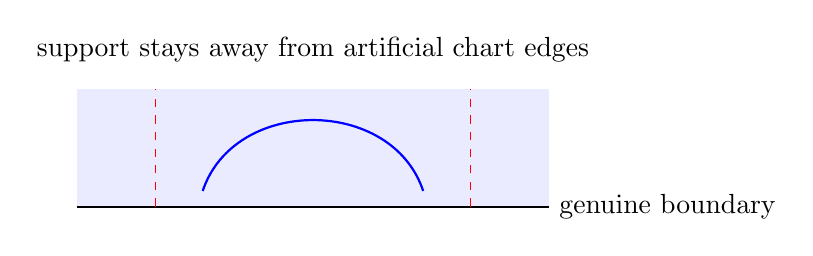
\begin{tikzpicture}
\fill[blue!8] (0,0) rectangle (6,1.5);
\draw[thick] (0,0)--(6,0) node[right] {genuine boundary};
\draw[dashed,red] (1,0)--(1,1.5) (5,0)--(5,1.5);
\draw[blue,thick] (1.6,.2) .. controls (2,1.4) and (4,1.4) .. (4.4,.2);
\node at (3,2) {support stays away from artificial chart edges};
\end{tikzpicture}
\end{center}
\begin{theorem}[External refinement theorem]
\label{thm:manifold-refinement-external}
Here second countability means a countable topological basis
(\cref{def:second-countable}); precompact means compact closure
(\cref{def:precompact-paracompact}). Every second-countable Hausdorff
smooth manifold, possibly with boundary, is
paracompact.  Given an open cover of \(M\), there are countable locally finite
families of open coordinate neighborhoods \(V_j\) and \(W_j\), with the
\(V_j\) covering \(M\), such that
\(\overline{V_j}\) is compact and
\[
\overline{V_j}\subseteq W_j\subseteq U_{\alpha(j)}
\]
for a suitable index \(\alpha(j)\in I\).
\end{theorem}

This is an external topological input. See Lee's second edition,
\cite[Theorem~1.15 and the coordinate-ball refinement in the proof of
Theorem~2.23, pp.~43--44; boundary adaptation in Exercise~2.24]{lee-smooth}.
The nested coordinate-neighborhood version stated here uses the same
shrinking of coordinate balls (half-balls at boundary points). We import
that refinement, not the smooth partition theorem: the bump construction,
normalization, and regrouping are proved below using Chapter~11.

\emph{Why the refinement can be nested.} First choose a countable locally finite cover $(O_i)$ by precompact
coordinate neighborhoods refining the given cover. Apply that statement
again using a basis of
smaller coordinate neighborhoods whose compact closures lie in some $O_i$.
Call the resulting cover $(V_j)$ and choose
\[
\overline{V_j}\subset W_j=O_{i(j)}.
\]
Local finiteness and compactness give
\[
\#\{j:V_j\cap\overline{O_i}\ne\varnothing\}<\infty.
\]
Consequently each $O_i$ is repeated only finitely often in $(W_j)$.
Local finiteness of $(O_i)$ then proves local finiteness of $(W_j)$.
Small coordinate balls or relative half-balls provide the required bases:
inside a prescribed open neighborhood, intersect with a chart and choose
a model ball of sufficiently small radius, with compact closure still
inside the chart image. Pulling it back gives the local refinement required
by \cref{def:topological-basis}; compactness of its closure is preserved by
the inverse chart. This
explains the nested formulation without importing a partition of unity.

\Needspace{16\baselineskip}
\begin{theorem}[Partition of unity]
\label{thm:partition-unity}
Let $M$ be a smooth manifold, possibly with boundary, and let
$(U_\alpha)_{\alpha\in I}$ be an open cover. There are smooth functions
$\rho_\alpha:M\to[0,1]$ whose supports form a locally finite family and
satisfy
\[
\operatorname{supp}(\rho_\alpha)\subseteq U_\alpha
\quad(\alpha\in I),\qquad
\sum_{\alpha\in I}\rho_\alpha=1.
\]
Such a partition of unity is \textbf{subordinate} to the cover: each
weight has its full closed support inside its assigned open set.
\end{theorem}
\begin{proof}
\textbf{Strategy.} Build bumps on the refined charts, normalize by their
positive sum, then regroup by the original cover.

\emph{Local bumps.} Apply the external refinement theorem
\cref{thm:manifold-refinement-external} to obtain
\[
\overline{V_j}\subseteq W_j\subseteq U_{\alpha(j)}.
\]

For a manifold with boundary, use boundary charts in this construction; the
smooth-extension convention in the definition of a manifold with boundary
makes the same Euclidean bump-function construction applicable.

For each $j$, let $\varphi_j:W_j\to O_j$ be its chart, with $O_j$
open in $\R^n$ or relatively open in $\mathbb H^n$. Write
$O_j=\widetilde O_j\cap\mathbb H^n$ in the boundary case, with
$\widetilde O_j$ open in $\R^n$; in the interior case use $\widetilde O_j=O_j$.
The coordinate set $K_j=\varphi_j(\overline{V_j})$ is compact in
$\widetilde O_j$. By \cref{lem:euclidean-cutoff}, choose a smooth
$b_j$ compactly supported there, with $0\leq b_j\leq1$ and $b_j=1$
near $K_j$.
Restrict to $O_j$, transfer by $\varphi_j$, and extend by zero outside
$W_j$ in $M$, obtaining $\chi_j$. Its support is compact inside $W_j$,
so this extension is smooth across artificial chart boundaries. At the
genuine boundary we retain the smooth Euclidean bump extension, which need
not be zero on the other side. Thus
\[
\chi_j\geq0,\qquad\chi_j>0\text{ on }V_j,\qquad
\operatorname{supp}\chi_j\subset W_j.
\]

\emph{Normalization.} Because the family \((W_j)\) is locally finite and
\(\operatorname{supp}(\chi_j)\subseteq W_j\), the family of supports
\((\operatorname{supp}(\chi_j))\) is locally finite.  Therefore the sum
\[
\chi=\sum_{j=1}^{\infty}\chi_j
\]
is smooth and well defined by \cref{lem:local-finiteness}; it is positive because the
\(V_j\) cover \(M\).  Set
\[
\rho_j=\frac{\chi_j}{\chi}.
\]
The denominator is positive, and local finiteness makes \(\chi\) smooth and
each quotient smooth.  The family \((\rho_j)\) is locally finite, satisfies
\[
\operatorname{supp}(\rho_j)\subseteq\operatorname{supp}(\chi_j)
\subseteq W_j\subseteq U_{\alpha(j)},
\]
and sums to one.

\emph{Regrouping.} For each original index \(\alpha\), define
\[
\rho_\alpha=\sum_{\{j:\alpha(j)=\alpha\}}\rho_j.
\]
These sums are locally finite, so the \(\rho_\alpha\) are smooth and the
regrouped family remains locally finite.  Moreover, by \cref{lem:local-finiteness}, a locally finite union of
closed sets is closed, and therefore
\[
\operatorname{supp}(\rho_\alpha)
\subseteq\bigcup_{\{j:\alpha(j)=\alpha\}}\operatorname{supp}(\rho_j)
\subseteq U_\alpha.
\]
Regrouping the locally finite sum also gives

\[
\sum_\alpha\rho_\alpha=1.
\]
  Thus the partition is subordinate to the
original cover.
\end{proof}

We can now reduce global questions to chart-supported local questions.
Local finiteness makes smooth sums legitimate on a whole neighborhood;
compact support makes only finitely many pieces relevant to an integral.

\begin{proof}[Completion of \cref{thm:orientation-top-form}]
Suppose $M$ is oriented and $n\geq1$. Choose a covering signed oriented
atlas, with constant sign on each chart domain $U_\alpha$. Its local
positive top form is
\[
\omega_\alpha=s_\alpha\,\dd x_\alpha^1\wedge\cdots\wedge\dd x_\alpha^n.
\]
On a positive chart $s_\alpha=1$, so this is the usual coordinate volume
form. The signs allow the same argument at both ends of an interval.
Choose a subordinate partition $(\rho_\alpha)$ by
\cref{thm:partition-unity}. Each $\rho_\alpha\omega_\alpha$ extends
smoothly by zero outside $U_\alpha$: every point outside that chart has
a neighborhood disjoint from the closed support of $\rho_\alpha$.
Inside a boundary chart its coefficients retain their smooth extensions
across the genuine face. Form the locally finite smooth sum
\[
\omega=\sum_\alpha\rho_\alpha\omega_\alpha.
\]
At $p$, evaluate on a positive tangent basis $\mathcal B_p$:
\[
\omega_p(\mathcal B_p)
=\sum_{\alpha:\rho_\alpha(p)>0}
\rho_\alpha(p)(\omega_\alpha)_p(\mathcal B_p)>0.
\]
Every displayed summand is positive, and at least one occurs because
the weights sum to one. Thus $\omega_p\ne0$.
For $n=0$, the function taking the chosen sign at each point is smooth
on the discrete manifold and nowhere zero. This proves the converse.
\end{proof}
Orientation has now produced a global top form. Integration will apply
the same localization idea to an arbitrary compactly supported top form,
using coordinate changes to prove that the resulting number is intrinsic.

The Euclidean compact cutoff used below is already available as
\cref{lem:euclidean-cutoff}; it was proved directly in Chapter~11.

\begin{lemma}[One extension near a compact coordinate set]
\label{lem:compact-boundary-extension}
Let $O$ be relatively open in $\mathbb H^n$, let $h$ be smooth on $O$
in the local-extension sense, and let $K\subset O$ be compact. There is
one smooth ambient extension of $h$ on a Euclidean neighborhood of $K$.
The assertion applies coefficient by coefficient to differential forms.
\end{lemma}
\begin{proof}
\textbf{Strategy.} Average finitely many local extensions with smooth
weights; on the half-space they all agree with $h$.

For each point of $K$ choose an ambient open neighborhood $V$ with
$V\cap\mathbb H^n\subset O$ on which a smooth extension exists. Choose
smaller balls with closed balls inside these neighborhoods and extract a
finite cover of $K$. The Euclidean cutoff construction in \cref{lem:euclidean-cutoff}
gives smooth nonnegative functions $b_1,\ldots,b_r$, compactly supported
in the respective neighborhoods $V_i$, whose sum $B$ is positive on $K$.
If $h_i$ is the corresponding local extension, extend $b_i h_i$ by zero
outside $V_i$; compact support makes this smooth. On the open set
$G=\{B>0\}$ define
\[
\widetilde h=\frac{\sum_{i=1}^r b_i h_i}{B}.
\]
This is smooth and $G$ contains $K$. On $G\cap\mathbb H^n$,
\[
\widetilde h=\frac{\sum_i b_i h}{B}=h,
\]
because each active local extension equals $h$ there. For a form,
first intersect the extension neighborhoods for its finitely many
coefficients, then use the same weights for all of them.
\end{proof}

\paragraph{Integrating in a boundary chart.}
Use the half-space form integral already defined in
\cref{def:halfspace-form-integral}. The compact boundary-extension lemma
supplies smooth ambient coefficients when needed for local Stokes;
zero extension still occurs only at artificial chart edges.

For an oriented zero-dimensional manifold, charts into $\R^0$ make
singletons open. A compact support is therefore finite, by its singleton
open cover. The signed finite-set convention above consequently defines
every compactly supported zero-dimensional integral.

Integration on manifolds is built locally from the familiar integration
on Euclidean space. With standard orientation and compactly supported
continuous coefficient $f$ on an open $V\subseteq\R^n$,
\[
\int_V f(u)\,\dd u^1\wedge\cdots\wedge\dd u^n
=\int_V f(u)\,\dd(u^1,\ldots,u^n).
\]
The right side is the scalar Riemann integral, defined by zero extension to
a containing rectangle; its volume notation is distinct from the wedge
product on the left. If $\sigma:V\to U\subset M$ is an orientation-preserving
chart parametrization and $\omega$ has compact support in $U$, then
\[
\int_U\omega=\int_V\sigma^*\omega.
\]
In the equal-dimensional Euclidean special case, let $\sigma:V\to U$
be a smooth change of variables between open subsets of $\R^n$.
Its derivative is square. In coordinates $x^1,\ldots,x^n$,
multilinearity and alternation give
\[
\begin{aligned}
\sigma^*(\dd x^1\wedge\cdots\wedge\dd x^n)
&=d\sigma^1\wedge\cdots\wedge d\sigma^n\\
&=\det D\sigma\,\dd u^1\wedge\cdots\wedge\dd u^n.
\end{aligned}
\]
The determinant measures the change in oriented volume. Forms retain its
sign; the unoriented scalar change-of-variables formula uses
$|\det D\sigma|$. An orientation-reversing parametrization therefore requires
a minus sign in the displayed integral identity when $U$ keeps its fixed
orientation. The chart signs in the following definition record exactly this.

\begin{definition}[Integration on an oriented manifold]\label{def:manifold-integral}
Let $M$ be an oriented $n$-manifold and let $\omega$ be a smooth $n$-form
with compact support.  Choose a partition of unity subordinate to oriented
coordinate charts. First localize: $\eta_\alpha=\rho_\alpha\omega$.
In coordinates extract the scalar coefficient $g_\alpha$ by
\[
(\varphi_\alpha^{-1})^*\eta_\alpha
=g_\alpha(u)\,du^1\wedge\cdots\wedge du^n.
\]
Define
\[
\int_M\omega
=\sum_\alpha s_\alpha\int_{\varphi_\alpha(U_\alpha)}
g_\alpha(u)\,\dd(u_1,\ldots,u_n).
\]
The sequence is: localize, express in coordinates, extract the scalar
top-degree coefficient, integrate, apply the orientation sign, and sum.
Equivalently, in compact form,
\[
\int_M\omega
=
\sum_\alpha s_\alpha\int_{\varphi_\alpha(U_\alpha)}
(\varphi_\alpha^{-1})^*(\rho_\alpha\omega).
\]
Here $s_\alpha$ is the coordinate-frame sign defined above; each written
coordinate integral uses the standard orientation of its Euclidean or
half-space model. Equivalently integrate without the explicit sign in
the correspondingly oriented model. Only finitely many supports
\(\operatorname{supp}(\rho_\alpha)\) meet the
compact set \(\operatorname{supp}(\omega)\).  Furthermore,
\[
\operatorname{supp}(\rho_\alpha\omega)
\subseteq
\operatorname{supp}(\rho_\alpha)\cap\operatorname{supp}(\omega)
\subseteq U_\alpha.
\]
This support is a closed subset of the compact set
\(\operatorname{supp}(\omega)\), so it is compact.  Its image under
\(\varphi_\alpha\) is therefore compact and contained in the chart image, open in Euclidean
space or relatively open in the half-space. Thus every nonzero summand is
the appropriate compactly supported coordinate integral defined above, and the displayed sum is finite.
\end{definition}

Two global decompositions are difficult to compare directly. Intersect
their localized chart pieces: each smaller piece lies in one chart from
each construction. The independence proof therefore follows the route
\[
\text{two choices}\to\text{common refinement}\to\text{overlap comparison}
\to\text{coordinate invariance}\to\text{reassembly}.
\]
\begin{proposition}[Well-definedness]
\label{prop:manifold-integral-well-defined}
The preceding integral is independent of the oriented charts and subordinate
partition of unity.
\end{proposition}
\begin{proof}
To compare two choices, compare both to a common refinement. Let
$(\rho_\alpha)$ and $(\sigma_\beta)$ be partitions subordinate to chart
families $(U_\alpha,\varphi_\alpha)$ and $(V_\beta,\psi_\beta)$.
Let $K=\operatorname{supp}(\omega)$, which is compact. By
\cref{lem:local-finiteness}, only finitely many supports in either family
meet $K$. Thus only finitely many products below can be nonzero.
Define $\eta_{\alpha\beta}=\rho_\alpha\sigma_\beta\omega$. Its support
is closed and is contained in
\[
K\cap\operatorname{supp}(\rho_\alpha)\cap\operatorname{supp}(\sigma_\beta)
\subseteq U_\alpha\cap V_\beta.
\]
It is therefore compact and lies within the chart overlap, so either chart
can integrate this same localized form.

For a chart-supported form $\theta$, write its signed coordinate integral as
\[
I_\alpha(\theta)=s_\alpha\int_{\varphi_\alpha(U_\alpha)}
(\varphi_\alpha^{-1})^*\theta,\qquad
J_\beta(\theta)=s_\beta\int_{\psi_\beta(V_\beta)}
(\psi_\beta^{-1})^*\theta.
\]
On the overlap the transition determinant has sign $s_\beta s_\alpha$.
The signed change-of-coordinates formula
(\cref{prop:open-form-invariance,cor:halfspace-change-variables}) therefore
gives $I_\alpha(\eta_{\alpha\beta})=J_\beta(\eta_{\alpha\beta})$,
including opposite coordinate signs. Consequently,
\[
\begin{aligned}
\sum_\alpha I_\alpha(\rho_\alpha\omega)
&=\sum_{\alpha,\beta}I_\alpha(\eta_{\alpha\beta})\\
&=\sum_{\alpha,\beta}J_\beta(\eta_{\alpha\beta})\\
&=\sum_\beta J_\beta(\sigma_\beta\omega).
\end{aligned}
\]
The first equality uses
\[
\sum_\beta\sigma_\beta=1
\]
 and linearity in a
fixed chart. The middle equality is the overlap formula just verified.
The last uses
\[
\sum_\alpha\rho_\alpha=1.
\]
 Compact support and local
finiteness make this a finite double sum, so no infinite rearrangement
is involved. Both choices give the same integral.
\end{proof}

\begin{example}[The circle integral using two chart-supported pieces]
Orient $S^1$ counterclockwise and restrict $\omega=-y\,\dd x+x\,\dd y$
from the plane. The angle parametrization $\gamma(t)=(\cos t,\sin t)$
has $\gamma^*\omega=\dd t$, but no single angle chart covers the circle.
Use $U_+=S^1\setminus\{(-1,0)\}$ with angles $t\in(-\pi,\pi)$ and
$U_-=S^1\setminus\{(1,0)\}$ with angles $t\in(0,2\pi)$.
Both angle coordinate frames have positive orientation.

Let $\theta$ be the smooth function from Chapter~8 that is zero on
$(-\infty,0]$ and
\[
e^{-1/s}
\]
 for $s>0$. For $(x,y)\in S^1$, define
\[
\rho_+(x,y)=\frac{\theta(x+1/2)}{\theta(x+1/2)+\theta(1/2-x)},
\qquad \rho_-=1-\rho_+.
\]
The denominator is positive: the two arguments cannot both be nonpositive.
These are smooth nonnegative weights summing to one.
The support of $\rho_+$ lies in
\[
\{x\geq-1/2\}\subset U_+,
\]
 and that
of $\rho_-$ lies in
\[
\{x\leq1/2\}\subset U_-.
\]
 Both supports are compact.
Thus this is an explicit subordinate partition of unity.
Put $r_\pm(t)=\rho_\pm(\gamma(t))$, which are $2\pi$-periodic. The
definition of manifold integration gives the two localized coordinate integrals
\[
\int_{S^1}\omega=\int_{-\pi}^{\pi}r_+(t)\,\dd t
+\int_0^{2\pi}r_-(t)\,\dd t.
\]
Their integrands vanish near the artificial endpoints of their respective
charts, as required by chart-supported integration. Split the first integral
at zero and substitute $s=t+2\pi$ on $[-\pi,0]$. Periodicity changes it to

\[
\int_0^{2\pi}r_+(s)\,\dd s.
\]
 Consequently
\[
\int_{S^1}\omega=\int_0^{2\pi}(r_++r_-)(t)\,\dd t
=\int_0^{2\pi}1\,\dd t=2\pi.
\]
The global definition reproduces the earlier line integral by adding two
chart-supported pieces; it never assumes a global angle coordinate.
\end{example}

\subsection{Smooth Euclidean Domains and the Riemann Integral}

The manifold integral should recover the ordinary multiple integral on
a smooth bounded Euclidean domain. To prove this, we must relate its
boundary charts to the Jordan boundary criterion and then compare the
two integrals after localization. We specify the class of domains first.

\label{sec:euclidean-integral-bridge}

For the classical corollaries, a \textbf{compact smooth domain}
$\Omega\subset\R^n$ ($n\geq1$) carries the smooth structure induced by
its Euclidean embedding. Interior points have identity coordinates.
At each boundary point there is a smooth ambient diffeomorphism
$\varphi:W\to O$ between open subsets of $\R^n$ with
\[
\varphi(W\cap\Omega)=O\cap\mathbb H^n,
\qquad
\varphi(W\cap\partial\Omega)=O\cap\{x_n=0\}.
\]
Its restriction is a boundary chart. Here $\partial\Omega$ is the
ordinary Euclidean boundary, which these charts identify with the manifold
boundary. We use the standard Euclidean orientation. This describes only
the concrete domains needed below; it assumes no theorem about the region
enclosed by an arbitrary simple closed curve.

\begin{proposition}[Smooth compact domains are Jordan measurable]
\label{prop:smooth-domain-jordan}
Every compact smooth Euclidean domain is Jordan measurable.
\end{proposition}
\begin{proof}
Its boundary is closed and bounded, hence compact. At each boundary point
choose a straightening chart as above and a small closed coordinate
rectangle $R=R'\times[-\delta,\delta]$ inside $O$, centered at that
point's coordinate on $x_n=0$. By the boundary-straightening identity,
the inverse image under $\varphi$ of the relative interior of the central
face $R'\times\{0\}$ is a relative neighborhood of the boundary point.
On the compact rectangle $R$, $D\psi$ is bounded, where
$\psi=\varphi^{-1}$. Since $R$ is convex, the mean-value estimate on
its segments makes $\psi$ Lipschitz there. The image of its central face is Jordan-null
by \cref{lem:lipschitz-box-face}. Choose finitely many of these boundary
neighborhoods covering $\partial\Omega$; their associated null face images
cover it. Thus $\partial\Omega$ is Jordan-null, and
\cref{prop:jordan-boundary-criterion} proves the assertion. In dimension
one the faces are points, already covered by the same lemma.
\end{proof}

\begin{proposition}[Agreement with the Euclidean Riemann integral]
\label{prop:manifold-riemann-agreement}
Let $\Omega\subset\R^n$ be a compact smooth domain with the standard
orientation, and let $f$ be smooth on a neighborhood of $\Omega$. Then
\[
\int_\Omega^{\mathrm{manifold}}
 f\,\dd x_1\wedge\cdots\wedge\dd x_n
=\int_\Omega^{\mathrm{Riemann}} f(\mathbf{x})\,\dd\mathbf{x}.
\]
\end{proposition}
\begin{proof}
Localize to the concrete ambient charts, use Chapter~12
to compare each pair of integrals, and add the finitely many identities.
No form of Stokes is needed. The scalar integral exists by
\cref{prop:smooth-domain-jordan,prop:continuous-jordan-extension}.

\emph{1. Choose finitely many coordinate neighborhoods and rectangle unions.}
Choose a partition of unity $\rho_\alpha$ subordinate to a finite cover
by the interior or straightening charts just described, shrinking the
charts to connected coordinate neighborhoods if necessary. Put
$h_\alpha=\rho_\alpha f$. Each $h_\alpha$ is continuous on $\Omega$
and has compact support inside its chart, so its scalar integral exists
too. Write $\psi_\alpha$ for the inverse ambient coordinate map and
$s_\alpha$ for the sign of its determinant. This determinant is nonzero
and has constant sign on the chosen neighborhood. Standard orientation
makes $s_\alpha$ precisely the chart-frame sign in manifold integration.

For one nonzero localized term, its compact coordinate support lies in a
finite union $E_\alpha$ of small closed grid rectangles inside the ambient
coordinate domain, contained in $\mathbb H^n$ in a boundary chart. To obtain
them, choose for each support point a ball of doubled radius inside the
coordinate domain, extract finitely many balls of the original radii, and
take a grid whose cell diameter is smaller than the least selected radius.
Every cell meeting the support then lies in one of the doubled balls. Only
finitely many such cells occur in their bounded union; in a boundary chart,
align the grid with $x_n=0$.
They cover a relative neighborhood of the coordinate support. Their union
is compact and Jordan measurable, and $\psi_\alpha(E_\alpha)\subset\Omega$.

\emph{2. Compare the localized integrals.}
\Cref{cor:jordan-nonlinear-change} first gives measurability of this image
and then, for the continuous function $h_\alpha$ on it, gives
\[
\int_{\psi_\alpha(E_\alpha)}h_\alpha(\mathbf{x})\,\dd\mathbf{x}
=\int_{E_\alpha}h_\alpha(\psi_\alpha(u))
       |\det D\psi_\alpha(u)|\,\dd u.
\]
The function vanishes outside its support. The scalar integral on the left
is therefore
\[
\int_\Omega h_\alpha:
\]
 the omitted difference is Jordan
measurable by \cref{prop:jordan-set-algebra} and has zero integrand.
The right side is also the coordinate integral over the whole chart,
using zero extension only across artificial edges. Indeed the coordinate
integrand vanishes outside $E_\alpha$. Meanwhile the pullback formula gives
\[
\psi_\alpha^*(h_\alpha\,\dd x_1\wedge\cdots\wedge\dd x_n)
=h_\alpha(\psi_\alpha(u))\det D\psi_\alpha(u)\,
 \dd u_1\wedge\cdots\wedge\dd u_n.
\]
The orientation sign gives, pointwise,
\[
s_\alpha\det D\psi_\alpha=|\det D\psi_\alpha|.
\]
Thus the localized manifold integral equals the localized scalar integral.

\emph{3. Sum the localized identities.}
Since
\[
\sum_\alpha\rho_\alpha=1
\]
 on $\Omega$,

\[
\sum_\alpha h_\alpha=f.
\]
 Sum the finitely many integral identities.
Linearity and the definition of manifold integration prove the proposition.
\end{proof}

\section{The General Stokes Theorem}

The local formula is now available in each chart. Smooth weights let us
add these formulas, and their derivative terms cancel because the weights
sum to one. Compact support will leave only finitely many contributions,
even if the manifold needs infinitely many charts.

For the boundary inclusion $\iota:\partial M\to M$, the notation

\[
\int_{\partial M}\omega
\]
 always means
\[
\int_{\partial M}\iota^*\omega.
\]

The pullback restricts the form to tangent directions of the boundary.

The general theorem unifies the Fundamental Theorem of Calculus, Green's
theorem, classical Stokes, and the divergence theorem: differentiating an
integrand over a region corresponds to integrating it over the oriented
boundary. The first three have already appeared in this chapter; the
following section recovers all four from the single identity below.

Recall that the integral is independent of charts and smooth weights
by \cref{def:manifold-integral,prop:manifold-integral-well-defined}.
Before asserting equality, both integrals must exist. By
\cref{lem:form-support}, compact support of a smooth $(n-1)$-form
$\omega$ gives compact support of the smooth top-degree form $d\omega$
on $M$ and of the smooth top-degree form $\iota^*\omega$ on $\partial M$.
The latter manifold and smooth inclusion were constructed in
\cref{prop:boundary-structure}. Thus the preceding integration definitions
(including dimension zero) supply both sides of the theorem.

\begin{theorem}[General Stokes theorem]
\label{thm:general-stokes}
Let $M$ be an oriented smooth $n$-manifold with boundary, $n\geq1$, and let $\omega$ be
a smooth $(n-1)$-form with compact support.  Then
\[
\int_M\dd\omega=\int_{\partial M}\omega.
\]
\end{theorem}
\begin{proof}
The proof follows the same local-to-global pattern used to define
manifold integration:
\[
\text{localize}\to\text{coordinates}\to\text{local Euclidean Stokes}
\to\text{reassemble}.
\]
All ingredients are now in place. The new payoff is that derivatives of
the smooth localization weights cancel, leaving the original derivative.
Choose a partition of unity subordinate to oriented manifold-with-boundary
charts that carry $M$ locally into \(\mathbb H^n\) and carry
\(\partial M\) into \(\set{x_n=0}\).  Compactness of
\(\operatorname{supp}(\omega)\) and local finiteness
show that only finitely many forms
\[
\rho_\alpha\omega
\]
are nonzero.  Each has compact support contained in the corresponding chart,
because
\(\operatorname{supp}(\rho_\alpha\omega)\subseteq
\operatorname{supp}(\rho_\alpha)\cap\operatorname{supp}(\omega)\).
By the product rule,
\[
\dd(\rho_\alpha\omega)
=
\dd\rho_\alpha\wedge\omega+\rho_\alpha\dd\omega.
\]
After summing, the first terms cancel because
\[
\sum_\alpha\dd\rho_\alpha
=
\dd\left(\sum_\alpha\rho_\alpha\right)=\dd1=0.
\]
This identity is legitimate because the partition is locally finite: near
each point both sums are finite, so exterior differentiation commutes with
the displayed sum.
In each local Stokes calculation multiply both sides by the chart sign
$s_\alpha$. Outward-normal-first transfers the same sign to its genuine
boundary integral, so the local formula remains valid for either orientation
of the coordinate model. It is therefore enough to prove the formula for a form supported in one
chart, where ``supported in'' means that its closure-based support lies in the
chart domain.

\begin{figure}[htbp]
\centering
\begin{tikzpicture}[font=\small,>=Stealth]

\fill[blue!7] (0,0) rectangle (4,2.4);
\draw[dashed,thick] (0,0) rectangle (4,2.4);
\filldraw[fill=blue!25,draw=blue] (2,1.2) ellipse (1.05 and .65);
\node at (2,1.2) {$\operatorname{supp}\eta$};
\node at (2,3) {interior chart};
\node[align=center] at (2,-.8) {zero near every artificial face\\local boundary integral $=0$};
\fill[blue!7] (6,0) rectangle (10,2.4);
\draw[dashed,thick] (6,0)--(6,2.4)--(10,2.4)--(10,0);
\draw[very thick,red!70!black] (6,0)--(10,0);
\filldraw[fill=blue!25,draw=blue] (7,0)--(9,0) .. controls (9,1.8) and (7,1.8) .. (7,0);
\node at (8,.55) {$\operatorname{supp}\eta$};
\node at (8,3) {boundary chart};
\node[align=center] at (8,-.8) {genuine face $x_n=0$ remains\\local boundary integral survives};
\node at (5,-1.8) {$\eta=\rho_\alpha\omega:\quad\text{artificial faces vanish; genuine faces reassemble into }\partial M$};

\end{tikzpicture}
\caption{Local Stokes applied to a chart-supported form. Compact support removes artificial boundary terms. Smooth extension across the genuine face need not be zero, and this is exactly where the manifold boundary integral comes from.}
\label{fig:local-global-stokes}
\end{figure}

\emph{Interior charts.} In an interior chart, the coordinate support is compact in the
open chart image.  Hence the coordinate representative vanishes on a
neighborhood of the artificial boundary of that image and extends smoothly by
zero to \(\R^n\).  Choose a rectangle whose interior contains the extended
support.  The extension vanishes near the rectangle boundary, so
\cref{thm:local-stokes} gives the formula with no manifold boundary
contribution.

\emph{Boundary charts.} In a boundary chart, \cref{lem:compact-boundary-extension}
combines the local smooth extensions into one smooth (not necessarily zero)
extension near the compact coordinate support, across
\[
x_n=0
\]
to a neighborhood in \(\R^n\).  Compact coordinate support permits zero
extension across the remaining artificial boundary of the coordinate image;
no zero extension is made across the genuine face \(x_n=0\).  Choose a
rectangle
\[
[a_1,b_1]\times\cdots\times[a_{n-1},b_{n-1}]\times[0,b_n]
\]
whose relative interior contains its coordinate support and whose artificial
faces are disjoint from it.  Using \cref{cor:compact-cutoff} in the ambient extension neighborhood to choose a cutoff equal to one near that support,
retain the smooth extension across \(x_n=0\) and extend by zero only across the
artificial faces; the resulting form vanishes near all of those faces.  Apply
\cref{thm:local-stokes} to the smooth extension.  Its only surviving boundary
term is the face \(x_n=0\), which is the coordinate representative of the
genuine manifold boundary.  The outward-normal-first convention gives
exactly the induced boundary sign.  Pullback compatibility
from \cref{prop:manifold-exterior-derivative} transfers each coordinate formula
back to the chart.

\emph{Reassembly.} Linearity and the cancellation above now give
\[
\begin{aligned}
\int_M d\omega
&=\sum_\alpha\int_M d(\rho_\alpha\omega)\\
&=\sum_\alpha\int_{\partial M}\iota^*(\rho_\alpha\omega)
=\int_{\partial M}\iota^*\omega.
\end{aligned}
\]
All nonzero contributions belong to a finite list, so the reassembly uses
only finite sums.
\end{proof}

\begin{corollary}[Integration by parts for differential forms]
\label{cor:forms-integration-by-parts}
Let \(M\) be an oriented smooth \(n\)-manifold with boundary, let
\[
0\leq p\leq n-1,
\]
let \(\alpha\) be a smooth \(p\)-form with compact support, and let
\(\beta\) be a smooth
\[
(n-p-1)\text{-form}.
\]
Then
\[
\int_M\dd\alpha\wedge\beta
=
\int_{\partial M}\alpha\wedge\beta
-
(-1)^p\int_M\alpha\wedge\dd\beta.
\]
\end{corollary}
\begin{proof}
The form
\[
\alpha\wedge\beta
\]
has degree \(n-1\) and compact support, so
\cref{thm:general-stokes} applies.  The graded Leibniz rule from
\cref{thm:exterior-derivative-rules} gives
\[
\dd(\alpha\wedge\beta)
=
\dd\alpha\wedge\beta
+
(-1)^p\alpha\wedge\dd\beta.
\]
Integrate this identity over \(M\), apply Stokes to its left side, and
rearrange.
\end{proof}

\begin{remark}[Three levels of integration by parts]
The same structural identity appears at three increasing levels of
generality:
\[
\begin{gathered}
\text{product rule plus the Fundamental Theorem of Calculus}\\
\Longrightarrow\ \text{one-variable integration by parts},\\
\text{one-variable integration by parts plus Fubini}\\
\Longrightarrow\ \text{the coordinatewise rectangular formula},\\
\text{graded Leibniz rule plus Stokes}\\
\Longrightarrow\ \text{integration by parts for forms}.
\end{gathered}
\]
The final formula is coordinate-free.  Green's identities and weak
formulations of partial differential equations are important later
descendants, but they require additional analytic machinery.
\end{remark}

\section{Classical Theorems Revisited}

These are now instances of one theorem. The form degree specifies the
dimension of integration; the exterior derivative specifies the interior
quantity. In three dimensions the flux form is the one already calculated
on surface patches. The general theorem additionally joins the chart pieces
consistently and handles arbitrary compact smooth oriented surfaces.

Choose the form and check its degree before applying Stokes:
\begin{center}
\begin{tabular}{lccc}
Formula & $\dim M$ & degree of $\omega$ & degree of $d\omega$\\\hline
FTC & 1 & 0 & 1\\
Green & 2 & 1 & 2\\
Surface Stokes & 2 & 1 & 2\\
Divergence & 3 & 2 & 3
\end{tabular}
\end{center}
A surface in $\R^3$ is still a \emph{two}-dimensional integration domain.
For $F=(F_1,F_2,F_3)$ the work and flux forms are different objects:
\[
\begin{aligned}
\alpha_F&=F_1\,\dd x+F_2\,\dd y+F_3\,\dd z,\\
\beta_F&=F_1\,\dd y\wedge\dd z+F_2\,\dd z\wedge\dd x
+F_3\,\dd x\wedge\dd y.
\end{aligned}
\]
Here $d\alpha_F$ encodes curl, while $d\beta_F$ encodes divergence.
Use the work one-form for circulation and the flux two-form for flux.

\begin{corollary}[Fundamental theorem of calculus]
For a smooth function $f$ on $[a,b]$,
\[
\int_a^b f'(x)\,\dd x=f(b)-f(a).
\]
\end{corollary}
\begin{proof}
Apply \cref{thm:general-stokes} to the oriented interval and the
$0$-form $f$. The interior integral is the ordinary Riemann integral
by \cref{prop:manifold-riemann-agreement}; the boundary integral has the
two endpoint signs.
\end{proof}

\begin{corollary}[Green's theorem]\label{cor:global-green}
Let $D\subseteq\R^2$ be a compact smooth Euclidean domain as in
``\nameref{sec:euclidean-integral-bridge},'' with the standard orientation, and let $P,Q$ be smooth on a neighborhood of $D$. The induced
boundary orientation is the usual positive orientation. Then
\[
\int_{\partial D}P\,\dd x+Q\,\dd y
=
\int_D
\left(
\frac{\partial Q}{\partial x}
-
\frac{\partial P}{\partial y}
\right)\dd x\,\dd y.
\]
\end{corollary}
\begin{proof}
Apply \cref{thm:general-stokes} to
\[
\omega=P\,\dd x+Q\,\dd y.
\]
Its derivative is
\[
(\partial Q/\partial x-\partial P/\partial y)
\,\dd x\wedge\dd y.
\]
 By \cref{prop:manifold-riemann-agreement}, the
manifold integral of this form is the displayed scalar Riemann integral.
\end{proof}

\begin{corollary}[Classical Stokes theorem]
Let $S$ be an oriented smooth compact surface with boundary in $\R^3$,
carrying the smooth structure induced by its Euclidean embedding, and let
\[
F=(P,Q,R)
\]
be smooth near $S$.  Then
\[
\int_{\partial S}P\,\dd x+Q\,\dd y+R\,\dd z
=
\int_S(\nabla\times F)\cdot n\,\dd S.
\]
\end{corollary}
\begin{proof}
Let $i:S\to\R^3$ and $j:\partial S\to S$ be the inclusions and let
$\alpha=P\,\dd x+Q\,\dd y+R\,\dd z$ on the ambient neighborhood.
The smooth form on $S$ is $i^*\alpha$. It has compact support because
$S$ is compact. Apply \cref{thm:general-stokes} to obtain
\[
\int_{\partial S}j^*i^*\alpha
=\int_S d(i^*\alpha)=\int_S i^*(d\alpha).
\]
The last equality uses commutation of pullback with $d$. Evaluation on
boundary velocities identifies the first integral with boundary work;
evaluation of $d\alpha$ on each oriented surface tangent pair gives
$(\nabla\times F)\cdot(\sigma_u\times\sigma_v)$, identifying the last
integral with curl flux by the parametrized formula.
\end{proof}

\begin{definition}[Flux in arbitrary dimension]\label{def:general-flux}
For a smooth vector field $F=(F_1,\ldots,F_n)$ on a Euclidean open set,
its flux form is the $(n-1)$-form
\[
\omega_F=\sum_{j=1}^n(-1)^{j-1}F_j\,
\dd x_1\wedge\cdots\wedge\widehat{\dd x_j}\wedge\cdots\wedge\dd x_n.
\]
For an oriented boundary with inclusion $\iota$, the notation
\[
\int_{\partial\Omega}F\cdot n\,\dd S
\quad\text{means}\quad\int_{\partial\Omega}\iota^*\omega_F.
\]
This defines the shorthand through form integration; no separate
hypersurface-measure construction is required here.
\end{definition}
For $n=3$ and an oriented patch $\sigma(u,v)$, evaluation gives
$\omega_F(\sigma_u,\sigma_v)=\det(F,\sigma_u,\sigma_v)
=F\cdot(\sigma_u\times\sigma_v)$ by \cref{prop:cross-product-identities}.
Thus the definition agrees with the earlier unit-normal flux formula.
For $n=1$, the flux form is the function $F_1$ and the signed endpoint
integral gives its value at the right endpoint minus its value at the left.

\begin{corollary}[Divergence theorem]
Let $\Omega\subseteq\R^n$ be a compact smooth Euclidean domain as in
``\nameref{sec:euclidean-integral-bridge},'' with the standard orientation, and let
\[
F=(F_1,\ldots,F_n)
\]
be smooth near $\Omega$. The induced boundary orientation is the usual
outward orientation. Then
\[
\int_{\partial\Omega}F\cdot n\,\dd S
=
\int_\Omega
\left(\sum_{j=1}^{n}\frac{\partial F_j}{\partial x_j}\right)\dd\mathbf{x}.
\]
\end{corollary}
\begin{proof}
Apply \cref{thm:general-stokes} to the flux form $\omega_F$ of
\cref{def:general-flux}. Its exterior derivative is

\[
(\sum_j\partial F_j/\partial x_j)\,\dd x_1\wedge\cdots\wedge\dd x_n:
\]

only the $j$th derivative of $F_j$ survives, and moving $\dd x_j$ past
$j-1$ factors cancels the coefficient sign. Its boundary integral is
the outward flux by definition. Finally,
\cref{prop:manifold-riemann-agreement} identifies the manifold integral
of its derivative with the scalar Riemann integral on the right.
\end{proof}




\Needspace{14\baselineskip}
\subsection*{Computational practice}
\begin{exercise}
Compute
\[
\int_\gamma x^2\,\dd s
\]
 on the quarter circle of radius $R>0$.
Compute the work of $(y,x)$ along $(t,3t)$, $0\leq t\leq1$, and its reverse.
\end{exercise}
\begin{exercise}
On the cylinder side of radius $R$ and height $h$, compute the scalar
surface integral of $z$ and the outward flux of $(2x,2y,z)$.
Explain which changes sign if orientation is reversed.
\end{exercise}

\Needspace{9\baselineskip}
\section*{Exercises}
\addcontentsline{toc}{section}{Exercises}

\begin{exercise}
Prove that
\[
\dim\Lambda^k((\R^n)^*)=\binom nk.
\]
\end{exercise}

\begin{exercise}
Let $\alpha,\beta$ be $1$-covectors.  Prove
\[
\alpha\wedge\beta=-\beta\wedge\alpha
\]
and give an example in which
\[
\alpha\wedge\beta\ne0.
\]
\end{exercise}

\begin{exercise}
For $\omega=x\,\dd y+y\,\dd z+z\,\dd x$, compute $\dd\omega$.
\end{exercise}

\begin{exercise}
Let
\[
\sigma(u,v)=(u^2-v^2,2uv).
\]
Compute
\[
\sigma^*(x\,\dd y-y\,\dd x).
\]
\end{exercise}

\begin{exercise}
Use \cref{thm:local-stokes} in dimension one to recover the Fundamental
Theorem of Calculus.
\end{exercise}

\begin{exercise}
Apply \cref{cor:forms-integration-by-parts} to the oriented interval
$[a,b]$ and the forms \(\alpha=u\) and \(\beta=v\) to recover the one-variable
integration-by-parts formula for smooth functions \(u\) and \(v\).
\end{exercise}

\begin{exercise}
For the unit square with its standard orientation, evaluate
\[
\int_{\partial Q}x\,\dd y
\]
and compare it with
\[
\int_Q\dd(x\,\dd y).
\]
\end{exercise}

\begin{exercise}
Let $D\subset\R^2$ be a compact smooth planar domain as in
\cref{cor:global-green}, with positively oriented boundary. Use that
theorem to prove
\[
\operatorname{area}(D)=\frac12\int_{\partial D}(x\,\dd y-y\,\dd x).
\]
\end{exercise}

\begin{exercise}
Use the divergence theorem to compute the outward flux of
\[
F(x,y,z)=(x,y,z)
\]
across the unit sphere.
\end{exercise}

\begin{exercise}
Explain why
\[
\dd^2=0
\]
is compatible with the boundary-of-boundary principle reflected in Stokes'
theorem. Distinguish this compatibility from a chain-level theorem, which
has not been developed here.
\end{exercise}

\begin{exercise}[Hypotheses and synthesis]
Test the scope of the preceding constructions.
\begin{enumerate}
\item Why does the full circular parametrization on $[0,2\pi]$ fail the
injective-patch hypothesis? Describe a valid subdivision.
\item Why can a two-sided curve in $[0,\infty)$ through zero not represent
the outward tangent vector there?
\item If $\rho_1+\rho_2=1$ near the support of $\omega$, expand
$\dd(\rho_1\omega)+\dd(\rho_2\omega)$ and identify the cancelling terms.
\item For $\sigma(u,v)=(u,v,u^2+v^2)$ on a triangle and $F=(-y,x,0)$,
verify patch Stokes by pulling back work to the triangle and computing curl
flux. State exactly why this does not by itself prove Stokes on a sphere.
\end{enumerate}
\end{exercise}

\begin{exercise}
For $\gamma(t)=(t,t^2)$ on $[0,1]$, compute the work of $F=(y,x)$.
Repeat with
\[
h(s)=(s+s^2)/2
\]
 by substitution and under reversal.
Explain why doubling the traversal is a different operation.
\end{exercise}
\begin{exercise}
Pull back $z\,\dd x\wedge\dd y$ by $(u,v)\mapsto(u,v,uv)$ and
integrate over $[0,1]^2$. Interpret the result as an oriented flux.
\end{exercise}
\begin{exercise}
For $\omega=x\dd y-y\dd x$, compute $\omega_{(1,2)}(3,4)$,
its pullback by $t\mapsto(t,t^2)$, and $\dd\omega$. State the type
of each answer and why a two-form pulled back to this curve is zero.
\end{exercise}
\begin{exercise}
Use the upper- and right-semicircle charts to transform a tangent
coordinate at
\[
(1/\sqrt2,1/\sqrt2).
\]
 Check the answer by differentiating
the corresponding parametrizations in the ambient plane.
\end{exercise}
\begin{exercise}
For a positively oriented interval verify its two endpoint chart signs
and Stokes for $f(x)=x^2$ on $[1,3]$. Explain why the endpoint at
$3$ can have a negative chart sign and a positive boundary sign.
\end{exercise}
\begin{exercise}
Construct two smooth weights on an overlapping cover of an interval by
normalizing cutoff functions. Check positivity of the denominator and
show directly that $\dd\rho_1+\dd\rho_2=0$.
\end{exercise}
\begin{exercise}
For a disk covered by two overlapping surface charts, explain which
chart edges disappear in the Stokes proof and which boundary remains.
Distinguish cancellation of derivatives of weights from zero extension
near an artificial chart edge.
\end{exercise}

\begin{exercise}
For two circle angle charts differing by $2\pi$ on an overlap component,
compute their transition derivative and check the tangent-vector equivalence
relation. Then replace an angle coordinate by twice that coordinate and
compute how a tangent-vector component changes without changing the vector.
\end{exercise}
\begin{exercise}
Use the coordinate transformation formula for $df_p$ to compare two source
and two target charts for $f:S^1\to S^1$, $f(\cos t,\sin t)=(\cos 2t,\sin 2t)$ locally.
Check explicitly that equivalent source representatives give equivalent outputs.
\end{exercise}
\begin{exercise}
Reconstruct the common-refinement proof for manifold integration. Identify
which support assumption permits each overlap integral and which hypothesis
makes the double sum finite.
\end{exercise}

\begin{exercise}
Let $f:S^1\to S^1$ be $f(x,y)=(x^2-y^2,2xy)$, and let $h(x,y)=x$
on $S^1$. In angle coordinates compute $f^*(\dd h)$ and $\dd(f^*h)$.
Repeat near the same point with source coordinate $s=2t$ and explain why
the two coordinate answers describe the same one-form.
\end{exercise}
\begin{exercise}
For the inclusion $\iota:S^1\to\R^2$ and $\alpha=x\,\dd y$, compute
$\iota^*\alpha$ in angle coordinates and verify
$\dd(\iota^*\alpha)=\iota^*(\dd\alpha)=0$.
Explain the role of $\Omega^2(S^1)=\{0\}$. Then reconstruct the overlap
identity that makes the manifold exterior derivative well defined.
\end{exercise}

\begin{exercise}[Charts, coordinate functions, and tangent columns]
On $S^1$ let $U=\{y>0\}$, $V=\{x>0\}$, $\varphi(x,y)=x$, and
$\psi(x,y)=y$. Write the full domains and codomains of both charts,
their inverses, and both overlap transitions. For a general chart
$\chi:W\to\R^n$, write its coordinate functions using projections.
At
\[
(\sqrt3/2,1/2)
\]
 convert $[\varphi,2]$ to its $\psi$ representative
and verify the equality of the two parametrized velocities in $\R^2$.
\end{exercise}
\begin{exercise}[Dual bases and a graph differential]
For $M=\{(x,y,x^2+y^2):(x,y)\in\R^2\}$, use graph coordinates to
construct the coordinate tangent and dual bases at $(1,2,5)$.
Verify all four duality evaluations. Compute the differential of the
inclusion $M\to\R^3$ on $[\varphi,(2,-1)]$ and explain which space
contains its input and which contains its output.
\end{exercise}
\begin{exercise}[Orientation from charts and forms]
Use the circle transition above to test the signs of the two coordinate
bases. Compute the coefficient of $x\,\dd y-y\,\dd x$ in each chart
on the first-quadrant overlap and check that it gives the same tangent
orientation. Verify the endpoint chart signs and boundary signs for
$[a,b]$ oriented by decreasing $x$. Finally explain, using
\cref{thm:orientation-top-form}, why a nonorientable manifold cannot
admit a nowhere-zero top form; no example of nonorientability is required.
\end{exercise}

\section{Perspective and Further Directions}
\label{sec:perspective-further-directions}
Differentiation, orientation, and integration meet in Stokes' theorem.
The subjects below develop different parts of that meeting. This section
is a map for further study;
Appendices~\ref{app:quotients}--\ref{app:cohomology} provide selected developed
continuations. Named later theorems in this section are unproved previews,
not prerequisites for the principal Chapters~1--13 route.

There are three overlapping starting points: topology leads toward general,
algebraic, and geometric topology; smooth manifolds lead toward differential
topology, differential geometry, Lie theory, and de Rham theory; analysis
leads toward function spaces, PDE, complex analysis, probability, and
geometric analysis. These are connections, not rigid disciplinary partitions.
\begin{center}
\begin{tabular}{p{.30\linewidth}p{.58\linewidth}}
\textbf{Starting mechanism}&\textbf{A developed bridge and later direction}\\[3pt]
Quotients and gluing&Appendix~\ref{app:quotients} $\to$ geometric topology\\
Constant-rank ideas&Appendix~\ref{app:submanifolds} $\to$ differential topology\\
Manifolds and algebra&Appendix~\ref{app:lie} $\to$ Lie theory\\
Forms and Stokes&Appendix~\ref{app:cohomology} $\to$ de Rham theory and topology\\
Analysis and geometry&PDE and variational methods $\to$ geometric analysis
\end{tabular}
\end{center}

\subsection*{General Topology}

The open-set language of Chapter~10 also describes spaces obtained by
identifying points. Appendix~\ref{app:quotients}, \emph{Quotient Spaces,
Gluing, and Classical Manifolds}, develops quotient topology
and its universal property, then applies them to circles, tori, the cylinder, the
M\"obius strip, the Klein bottle, and real projective spaces. This developed
continuation makes the chapter's gluing pictures rigorous while keeping the main
analysis-to-Stokes development independent of quotient topology.

The external refinement theorem used for partitions of unity is another
point where topology does work that coordinate calculations alone cannot.
A topology course develops product and quotient spaces, separation axioms,
compactness, connectedness, paracompactness, and criteria for metrizability.
That broader theory explains why certain global constructions are possible.

General topology supplies the language for constructing and comparing
spaces. Algebraic topology asks what global information can be extracted
from them by assigning algebraic invariants.

\subsection*{Algebraic Topology}

\phantomsection\label{sec:algebraic-topology-preview}
Algebraic topology assigns algebraic invariants to topological spaces and
continuous maps, transferring geometric questions to algebra, where
computation and comparison are often more tractable. This deliberately loses information: distinct
spaces may have the same invariant. The art is to forget enough structure
to obtain something computable while retaining enough to detect the
phenomenon of interest. Fundamental groups, homology, cohomology, and Euler
characteristics are useful invariants, not complete classifications.
The working pattern is to construct an invariant that respects continuous
deformation, compute it for model spaces, and then deform or compare a new
problem until those computations apply:
\[
\text{spaces and continuous maps}
\longrightarrow\text{groups, chain complexes, and cohomology groups}.
\]
The definitions below make this philosophy concrete; all landmark results
are unproved previews and remain outside the analysis-to-Stokes route.

\begin{definition}[Homotopy and homotopy equivalence]
For continuous $f,g:X\to Y$, a \textbf{homotopy} from $f$ to $g$ is a
continuous map $H:X\times[0,1]\to Y$ with
\[
H(x,0)=f(x),\qquad H(x,1)=g(x)\quad(x\in X).
\]
Write $f\simeq g$. Spaces $X,Y$ are \textbf{homotopy equivalent}, written
$X\simeq Y$, if continuous maps $f:X\to Y$ and $g:Y\to X$ satisfy
\[
g\circ f\simeq\operatorname{id}_X,\qquad f\circ g\simeq\operatorname{id}_Y.
\]
\end{definition}
Homotopy formalizes continuous deformation of maps. Homotopy equivalence
is weaker than homeomorphism: for instance $\R^n$ contracts to a point
by $H(\mathbf{x},t)=(1-t)\mathbf{x}$, but is not homeomorphic to a point for $n\geq1$.
It forgets some local structure while retaining global shape information.

\begin{definition}[Based loops and the fundamental group]
A \textbf{path} is a continuous map $\gamma:[0,1]\to X$; its endpoints
are $\gamma(0)$ and $\gamma(1)$. Path homotopies keep both endpoints fixed.
Fix $x_0\in X$. A \textbf{based loop} is a path with
$\gamma(0)=\gamma(1)=x_0$. A \textbf{based homotopy} from $\gamma_0$
to $\gamma_1$ is a continuous $H:[0,1]^2\to X$ satisfying
\[
\begin{gathered}
H(s,0)=\gamma_0(s),\quad H(s,1)=\gamma_1(s),\\
H(0,t)=H(1,t)=x_0\quad\text{for every }s,t\in[0,1].
\end{gathered}
\]
Thus the basepoint stays fixed throughout the deformation. Define
\[
(\alpha*\beta)(s)=
\begin{cases}\alpha(2s),&0\leq s\leq1/2,\\
\beta(2s-1),&1/2\leq s\leq1,
\end{cases}
\quad e_{x_0}(s)=x_0,\quad \alpha^{-1}(s)=\alpha(1-s).
\]
Concatenation traverses $\alpha$ first and then $\beta$. The
\textbf{fundamental group} is
\[
\pi_1(X,x_0)=\{\text{based loops at }x_0\}/\text{based homotopy},
\qquad [\alpha][\beta]=[\alpha*\beta].
\]
\end{definition}
\textbf{Group structure (unproved preview).} Based homotopy is an
equivalence relation, this product is well defined, and it makes
$\pi_1(X,x_0)$ a group with identity $[e_{x_0}]$ and inverse
$[\gamma]^{-1}=[\gamma^{-1}]$. The loops $(\alpha*\beta)*\gamma$ and
$\alpha*(\beta*\gamma)$ generally have different parametrizations;
they are based-homotopic, which gives associativity on classes.
The symbol $\pi_1$ denotes a group, whereas Appendix~\ref{app:quotients}'s $\pi$ denotes
a projection map.

Continuous pointed maps induce group homomorphisms by
$[\gamma]\mapsto[f\circ\gamma]$. Composing a based homotopy with $f$
proves representative independence, and composition respects concatenation.

\paragraph{Landmark examples (unproved previews).}
For $n\geq1$ and any basepoint in the indicated spaces,
\[
\pi_1(\R^n,x_0)=0,\qquad \pi_1(S^1,x_0)\cong\Z,\qquad
\pi_1(T^2,x_0)\cong\Z^2.
\]
Euclidean loops contract to a point. On the circle the integer counts
winding; on the torus the two integers count winding in the circular
directions of Figure~\ref{fig:embedded-torus}. In a path-connected space,
a chosen connecting path gives an isomorphism between groups at different
basepoints (unproved preview); that isomorphism need not be canonical
without the path choice.

\paragraph{Building a space one dimension at a time.}
Appendix~\ref{app:quotients} glues edges of simple domains. Cell attachment
extends this idea to disks in successive dimensions.
\begin{definition}[Cells, skeleta, and CW complexes]
Put $D^n=\{\mathbf{x}\in\R^n:\|\mathbf{x}\|\leq1\}$ and, for $n\geq1$,
$S^{n-1}=\partial D^n$. An $n$-cell is a copy of the open ball
$\operatorname{int}D^n$; a $0$-cell is a point.
Start with a discrete set $X^0$ of $0$-cells. Given continuous
\textbf{attaching maps} $\phi_\alpha:S^{n-1}\to X^{n-1}$, form
\[
X^n=\left(X^{n-1}\sqcup\coprod_\alpha D^n_\alpha\right)/{\sim},
\qquad z\sim\phi_\alpha(z)\quad(z\in\partial D^n_\alpha).
\]
The disjoint union carries the topology in which a subset is open exactly
when its intersection with each summand is open; the displayed
identification is then given the quotient topology.
The canonical maps from the attached disks into $X$ are the
\textbf{characteristic maps} $\varphi^n_\alpha:D^n_\alpha\to X$.
Each maps its interior homeomorphically onto its cell $e^n_\alpha$;
these cells partition $X$. Here ``open cell'' means a copy of an open
ball, not necessarily an open subset of $X$.
The \textbf{$n$-skeleton} $X^n$ is the union of all cells of dimension
at most $n$, giving $X^0\subseteq X^1\subseteq\cdots$.
A \textbf{CW complex} is the resulting Hausdorff space

\[
X=\bigcup_{n\geq0}X^n
\]
 with these conditions:
\begin{enumerate}
\item \textbf{Closure finiteness (C):} the closure of each cell meets only
finitely many cells.
\item \textbf{Weak topology (W):} $A\subseteq X$ is closed exactly when
its inverse image under every characteristic map $D^n_\alpha\to X$
(the map from the attached disk) is closed in that disk.
\end{enumerate}
It is \textbf{finite} if it has finitely many cells in total.
\end{definition}
The attaching map may identify different boundary points; a closed cell
need not itself be a disk. In the finite examples below the topology is
precisely that obtained from the displayed attachments.

\begin{example}[Cell structures for familiar quotients]
The following standard cell descriptions connect to Appendix~\ref{app:quotients}; their
general existence identifications are previews, not new prerequisites.
\begin{itemize}
\item $S^1$ has one vertex and one $1$-cell: attach both endpoints of an
interval to that vertex, as in \cref{sec:quotient-circle}.
\item For $n\geq1$,
\[
S^n\cong D^n/\partial D^n
\]
 by
\cref{sec:quotient-sphere} (Figure~\ref{fig:quotient-sphere}), so
one $0$-cell and one $n$-cell suffice. Separately, $S^0$ has two $0$-cells.
\item For $T^2$, the square has one vertex class, two edge classes $a,b$,
and one $2$-cell. Let $a$ follow increasing $x$ on horizontal edges and
$b$ increasing $y$ on vertical edges. Counterclockwise traversal from
$(0,0)$ reads $aba^{-1}b^{-1}$. Thus there is one $0$-cell, two $1$-cells,
and one $2$-cell, agreeing with \cref{sec:quotient-torus}.
The relation to the fundamental group is an \emph{unproved preview}:
\[
\pi_1(T^2)\cong\langle a,b\mid aba^{-1}b^{-1}=1\rangle\cong\Z^2.
\]
Here the presentation means that the generators commute, with no further
relations; its derivation requires later tools.
\item $\mathbb{RP}^n$ has one cell in every dimension $0,\ldots,n$
(unproved preview). This cell structure can be understood from the filtration
\[
\mathbb{RP}^0\subset\mathbb{RP}^1\subset\cdots\subset\mathbb{RP}^n
\]
together with the antipodal sphere model illustrated in
Figure~\ref{fig:projective-sphere}.
Geometrically, build $S^k$ from its equatorial $S^{k-1}$ and two open
hemispheres, starting with the two points of $S^0$. Antipodal cells
occur in pairs in every dimension; identifying each pair leaves one
cell in each dimension $0,\ldots,n$. The complement
of $\mathbb{RP}^{k-1}$ in $\mathbb{RP}^k$ is its affine $k$-cell.
\item The figure eight $S^1\vee S^1$, formed by identifying one point
of each circle, has one vertex and two $1$-cells. At the vertex four
branches meet; it is not a $1$-manifold. CW complexes extend well beyond manifolds.
\end{itemize}
\end{example}

\begin{definition}[Euler characteristic]
For a finite CW complex with $c_k$ cells of dimension $k$, define
\[
\chi(X)=\sum_{k\geq0}(-1)^k c_k.
\]
\end{definition}
For a finite two-dimensional CW complex put $V=c_0$, $E=c_1$, and
$F=c_2$. Then the definition specializes to
\[
\boxed{\chi(X)=V-E+F.}
\]
This recovers the classical Euler formula for finite cell decompositions
of surfaces: $\chi(S^2)=2$ whereas $\chi(T^2)=0$; the value is not always $2$.
The cell structures just displayed give
\[
\begin{aligned}
\chi(S^1)&=1-1=0,&\chi(S^2)&=1+1=2,\\
\chi(S^n)&=1+(-1)^n,&\chi(T^2)&=1-2+1=0,\\
\chi(\mathbb{RP}^n)&=\sum_{k=0}^n(-1)^k
=\begin{cases}1,&n\text{ even},\\0,&n\text{ odd}.\end{cases}
\end{aligned}
\]
The Klein square likewise has one vertex, two edges, and one face, so
$\chi(K)=1-2+1=0$.
\textbf{Invariance (unproved preview).} If a space admits two finite CW
decompositions, their alternating cell counts agree. Thus $\chi$ is an
invariant of the space rather than its chosen cell structure. In particular,
$\chi(S^2)\ne\chi(T^2)$ rules out a homeomorphism. But
$\chi(S^1)=\chi(T^2)=0$: useful information need not be complete information.

\paragraph{Singular homology: cycles modulo boundaries.}
We now choose real coefficients throughout, to prepare for the comparison
with differential forms. The integral version instead uses free abelian groups.
\begin{definition}[Singular chains and homology]
The standard $k$-simplex is
\[
\Delta^k=\{(t_0,\ldots,t_k)\in\R^{k+1}:t_i\geq0,\ \sum_i t_i=1\}.
\]
For $k\geq1$ and $0\leq i\leq k$, the \textbf{face map}
$\delta_i:\Delta^{k-1}\to\Delta^k$ inserts zero as coordinate $i$.
A \textbf{singular $k$-simplex} in $X$ is a continuous map
$\sigma:\Delta^k\to X$. Let $C_k(X;\R)$ be the free real vector space on
these maps: its elements are finite formal linear combinations of them.
For $k\geq1$, define the boundary on generators and extend linearly:
\[
\partial_k:C_k(X;\R)\to C_{k-1}(X;\R),\qquad
\partial_k\sigma=\sum_{i=0}^k(-1)^i\sigma\circ\delta_i.
\]
Put $C_{-1}=0$ and $\partial_0=0$.
The \textbf{boundary identity (unproved preview)} is
$\partial_{k-1}\partial_k=0$. Thus boundaries are cycles, and the following
quotient is defined:

\[
\begin{aligned}
Z_k(X;\R)&=\ker\partial_k,\qquad
B_k(X;\R)=\operatorname{im}\partial_{k+1},\\
H_k(X;\R)&=Z_k(X;\R)/B_k(X;\R).
\end{aligned}
\]
\end{definition}
The inclusion $B_k\subseteq Z_k$ follows from the boundary identity.
Cycles have no boundary; boundaries are cycles
coming from one dimension higher. Homology records cycles modulo those
already bounding a chain. A singular simplex need not be injective, and
these chain spaces generally have many more generators than a cell structure.

\paragraph{Continuous maps induce homology maps.}
For continuous $f:X\to Y$, put $f_*(\sigma)=f\circ\sigma$ on singular
simplices and extend linearly to chains. The boundary formula gives
$\partial f_*=f_*\partial$, so cycles map to cycles and boundaries to
boundaries. Hence there is an induced linear map
\[
f_*:H_k(X;\R)\to H_k(Y;\R),\qquad [c]\longmapsto[f_*c].
\]
Again $(g\circ f)_*=g_*\circ f_*$ and $(\operatorname{id}_X)_*=\operatorname{id}$.
The passage from continuous maps to linear maps on chains, then to linear
maps on homology, realizes the opening philosophy concretely.

\begin{definition}[Real singular cohomology]
Put $C^k(X;\R)=\operatorname{Hom}_{\R}(C_k(X;\R),\R)$ and
\[
\delta^k:C^k\to C^{k+1},\qquad
(\delta^k\lambda)(c)=\lambda(\partial_{k+1}c).
\]
Then $\delta^{k+1}\delta^k=0$ by the boundary identity. With $C^{-1}=0$, define
\[
H^k_{\mathrm{sing}}(X;\R)=\ker\delta^k/\operatorname{im}\delta^{k-1}.
\]
\end{definition}
\textbf{Invariance (unproved preview).} Homotopy equivalent spaces have
isomorphic singular homology and cohomology groups. These definitions
therefore supply topological invariants, not just algebra attached to a presentation.

For a finite CW complex, the further identity

\[
\chi(X)=\sum_k(-1)^k\dim H_k(X;\R)
\]
 is an unproved preview.
Cellular homology makes this computationally useful: it uses one generator
per cell and boundary maps determined by the attachments, not just by cell
counts. A later course proves agreement with singular homology.
Hatcher~\cite{hatcher-topology} provides further reading for these optional
previews. Xiao's lecture notes~\cite{xiao-topology-notes} supply a supplementary
pedagogical benchmark for the progression through maps, homotopy, chains,
and CW examples; the full course is not imported here.
The later ``\nameref{sec:de-rham-preview}'' discussion compares
real singular cohomology with the differential forms already developed.

\subsection*{Geometric Topology}

\phantomsection\label{sec:geometric-topology-preview}
Geometric topology studies manifolds and related spaces through their
geometric realization, decomposition, and global topological structure.
Its working pictures involve cutting, gluing, decomposition, embedding,
and isotopy, meaning a deformation through embeddings. The surfaces in
Appendix~\ref{app:quotients} are an accessible starting point: one can
ask how a cut exposes a handle, or whether two placements of a curve can
be deformed into one another without crossings. Dimensions three and four
contain especially rich phenomena beyond this introductory picture.

Chapter~10 supplies the topological language; Appendix~\ref{app:quotients} supplies actual
quotient and gluing constructions; algebraic topology supplies invariants
with which to test them. Algebraic topology emphasizes extracting algebraic
invariants, while geometric topology emphasizes understanding the spaces
through their geometric and topological structure. These emphases overlap:
an invariant can obstruct an embedding or distinguish two constructions.
No classification theorem for surfaces or higher-dimensional manifolds is
assumed here.

\subsection*{Differential Topology}

\phantomsection\label{sec:differential-topology-preview}
Differential topology studies smooth manifolds and smooth maps through
their qualitative and global behavior, emphasizing properties that persist
under appropriate smooth deformations. Its entry point is
\[
\text{local differential information}\longrightarrow
\text{global topology of smooth maps and manifolds}.
\]
Appendix~\ref{app:submanifolds} supplies immersions, submersions,
embeddings, regular values, and the constant-rank theorem. Later questions
include: how typical are regular values; when do two submanifolds meet
in the expected dimension; and how does the topology of a level set change
as its level crosses a critical value?

Sard's theorem, transversality and intersection theory, degree theory,
indices of vector fields, Morse theory, and cobordism develop these
questions beyond Appendix~\ref{app:submanifolds}'s scope. Differential geometry often adds
metrics and curvature, while differential topology emphasizes smooth
structure and smooth maps at a more topological level. This is a useful
distinction of emphasis, with substantial overlap between the subjects.

\subsection*{Differential Geometry}

Tangent spaces tell us what directions are available, but do not assign
lengths or angles. A \textbf{Riemannian metric} on a smooth manifold $M$ is
a family
\[
g_p:T_pM\times T_pM\to\R\qquad(p\in M)
\]
of positive-definite inner products, varying smoothly: in each chart the
functions
\[
g_{ij}(p)=g_p((\partial/\partial x^i)|_p,
(\partial/\partial x^j)|_p)
\]
 are smooth. For a smooth curve $\gamma$,
write
\[
\dot\gamma(t)=d\gamma_t(\partial/\partial t).
\]
 Its speed and length are
\[
\norm{\dot\gamma(t)}_g=
\sqrt{g_{\gamma(t)}(\dot\gamma(t),\dot\gamma(t))},\qquad
L(\gamma)=\int_a^b\norm{\dot\gamma(t)}_g\,dt.
\]
Piecewise smooth curves use the sum of the lengths of their pieces.

On $S^2$, the inclusion $i:S^2\to\R^3$ gives
$g_p(v,w)=di_p(v)\cdot di_p(w)$, recovering the usual surface metric.
For example $\gamma(t)=(\cos t,\sin t,0)$ has unit speed, so one full
equatorial circuit has length $2\pi$. The sphere's nonconstant geodesics
are great circles with constant-speed parametrizations (unproved preview).
Geodesics are curves whose motion has no intrinsic acceleration; the
shorter great-circle arcs locally minimize length, though a whole great
circle does not minimize between its repeated endpoints.

Orientation and Stokes required no Riemannian metric; a metric adds lengths
and angles. A later course follows the route
\[
\text{connections}\longrightarrow\text{covariant differentiation}
\longrightarrow\text{geodesics}\longrightarrow\text{curvature}.
\]
These notions describe how directions at nearby points can be compared and
how intrinsic geometry differs from that of Euclidean space.


Appendix~\ref{app:submanifolds}, \emph{Submanifolds}, develops the smooth
geometric consequences of inverse, implicit, and constant-rank theory
before any metric is imposed. Appendix~\ref{app:lie}, \emph{Lie Groups
and Lie Algebras}, gives another setting for geometry, in which smooth
structure coexists with group multiplication. Lie theory has its own
algebraic questions, as the next direction explains.

\subsection*{Lie Theory}

\phantomsection\label{sec:lie-theory-preview}
The route $\text{smooth manifolds}+\text{groups}\to\text{Lie groups}
\to\text{Lie algebras}$ makes continuous symmetry accessible to linear
algebra. Appendix~\ref{app:lie}, \emph{Lie Groups and Lie Algebras},
develops translations, the tangent space at the identity, the bracket,
and concrete matrix exponentials. The circle and the additive line already
show why local tangent information and global group structure are different
questions. Further study leads to representation theory, symmetry in
differential equations, and group actions in geometry. These connections
extend well beyond Riemannian geometry.

\subsection*{De Rham Theory}

\phantomsection\label{sec:de-rham-preview}
The equation $d^2=0$ gives $\operatorname{im}d\subseteq\ker d$.
How far is that inclusion from equality? The quotient

\[
H^k_{\mathrm{dR}}(M)=\ker d/\operatorname{im}d,
\]
 with the maps in
degrees $k$ and $k-1$, records closed forms modulo exact forms.
The angular form on the punctured plane is locally a derivative but has
nonzero integral around the missing point, so it cannot be globally exact.
Appendix~\ref{app:cohomology}, \emph{de Rham Cohomology}, develops this
obstruction, proves local exactness, and computes the circle and the two
degree-one torus directions. Integration and Stokes connect these classes
to topology. The de Rham theorem, stated there without proof, identifies
them with real singular cohomology. This continuation needs forms and
Stokes, not a Riemannian metric.

\subsection*{Measure Theory and Lebesgue Integration}

Chapters~9 and~12 controlled integrals by finite partitions and Jordan
content. Limits of functions and countable decompositions suggest a more
flexible collection of sets on which size can be assigned.

A \textbf{$\sigma$-algebra} on a set $X$ is a family
$\mathcal A\subseteq\mathcal P(X)$ satisfying
\[
X\in\mathcal A,\qquad E\in\mathcal A\Longrightarrow X\setminus E\in\mathcal A,
\qquad (E_j)_{j\geq1}\subseteq\mathcal A
\Longrightarrow\bigcup_{j=1}^{\infty}E_j\in\mathcal A.
\]
A \textbf{measure} on this family is a map
\[
\mu:\mathcal A\to[0,\infty],\qquad \mu(\varnothing)=0,
\]
with countable additivity: for pairwise disjoint $E_j\in\mathcal A$,
\[
\boxed{\mu\left(\bigsqcup_{j=1}^{\infty}E_j\right)
=\sum_{j=1}^{\infty}\mu(E_j).}
\]
The triple $(X,\mathcal A,\mu)$ is the setting for Lebesgue integration.
Countable additivity on a $\sigma$-algebra supplies the flexibility absent
from Jordan content: the allowed sets remain allowed under countable unions.
Lebesgue measure on $\R^n$ extends the usual volumes of boxes.

\Needspace{14\baselineskip}
Here is one landmark result, \textbf{Dominated Convergence (unproved
preview)}. For measurable real functions $f_j,f$ on a measure space, suppose
\[
f_j\to f\quad\text{almost everywhere},\qquad
|f_j|\leq g\quad\text{almost everywhere for every }j,\qquad
\int_X g\,d\mu<\infty,
\]
where $g\geq0$ is measurable. Then
\[
\boxed{\int_X|f|\,d\mu<\infty,\qquad
\lim_{j\to\infty}\int_X f_j\,d\mu=\int_X f\,d\mu.}
\]
The vocabulary in this preview has precise later meanings: measurable real
functions have measurable inverse images of open sets; ``almost everywhere''
allows failure on a set of measure zero; and $L^1$ denotes integrable
functions, with functions equal almost everywhere identified.

Uniform convergence in the Riemann theory controls errors at every point.
The one-dimensional Arzel\`a theorem proved earlier also allows uniformly
bounded pointwise convergence, but assumes integrability of the limit.
The displayed Lebesgue theorem instead derives integrability of the limit
from measurable convergence and an integrable dominating function.

For a concrete preview, the rationals in $[0,1]$ form a countable set of
Lebesgue measure zero. Thus
\[
\int_0^1\mathbf1_{\Q}(x)\,dx=0\qquad\text{(Lebesgue integral)},
\]
although every nondegenerate interval contains rational and irrational
points, so its lower and upper Riemann sums remain $0$ and $1$.
A later course constructs this integral and proves its convergence theorems;
see Knapp~\cite[Theorem~5.30]{knapp-basic-real} (digital second edition).

\subsection*{Functional Analysis}

Chapter~10 studied norms on finite-dimensional spaces, and Chapter~6
studied limits of functions. Functional analysis treats whole function
spaces as geometric spaces on which linear operators act.
\[
\begin{gathered}
\boxed{\text{Banach space}=\text{complete normed vector space},}\\[4pt]
\boxed{\text{Hilbert space}=\text{complete inner-product space}.}
\end{gathered}
\]
Completeness refers to the metric induced by the norm; for a Hilbert space
the norm is $\norm{x}=\sqrt{\langle x,x\rangle}$. A central real example is
\[
C([a,b]),\qquad \norm{f}_\infty=\max_{x\in[a,b]}|f(x)|.
\]
This is Banach: a Cauchy sequence in the maximum norm has pointwise limits
by completeness of $\R$, the same Cauchy estimate makes convergence uniform,
and the uniform limit is continuous. Its vectors are functions, so its
dimension is infinite when $a<b$.

Finite-dimensional intuition has limits. Norms need not be equivalent:
on $C([0,1])$,
\[
\int_0^1|f|
\]
 is another norm, but the continuous functions
$f_j(x)=\max(1-jx,0)$ have maximum norm $1$ and integral norm
\[
1/(2j).
\]

Closed bounded sets need not be compact, either. Continuous unit-height
bumps with disjoint supports in $(0,1)$ have pairwise maximum-norm distance
$1$, so finitely many open balls of radius
\[
1/3
\]
 cannot cover the closed unit ball.

The \textbf{Riesz representation theorem for Hilbert spaces (unproved
preview)} gives a striking survival of finite-dimensional duality.
For a real Hilbert space $H$, let $H^*$ mean its \emph{continuous} linear
functionals, not the unrestricted algebraic dual. Then
\[
\forall\ell\in H^*,\quad\exists!y\in H:\qquad
\boxed{\ell(x)=\langle x,y\rangle\quad(x\in H).}
\]
This extends the finite-dimensional identification of a covector with a
gradient once an inner product is chosen. A later course studies bounded
operators, spectral theory, and weak convergence in such spaces; see
Knapp~\cite[Theorem~12.5]{knapp-basic-real} (digital second edition).

The function-space viewpoint also prepares the variational problems described
under Geometric Analysis below.

\subsection*{Complex Analysis}

The real power-series and differentiation chapters suggest replacing $\R$
by $\C$. For an open $U\subseteq\C$ and $f:U\to\C$, complex
differentiability at $z\in U$ means existence of
\[
f'(z)=\lim_{h\to0,\ h\in\C}\frac{f(z+h)-f(z)}h.
\]
The increment approaches zero through \emph{every} complex direction. A
function complex differentiable at every point of $U$ is called
\textbf{holomorphic} on $U$.

For $f=u+iv$ with $u,v$ continuously real differentiable on $U$, the
Cauchy--Riemann criterion (preview) says that holomorphicity is equivalent to
\[
u_x=v_y,\qquad u_y=-v_x\quad\text{throughout }U.
\]
These equations say the real derivative matrix is multiplication by one
complex number. For $f(z)=\overline z$, the difference quotient is $1$
along real increments and $-1$ along imaginary increments; this real
smooth map is not complex differentiable.

\textbf{Cauchy's integral formula (unproved preview)} states: if $f$ is
holomorphic on an open neighborhood of the closed disk
$\overline{B(a,R)}$, and $\gamma$ is its positively oriented boundary circle,
then for $|z-a|<R$,
\[
\boxed{f(z)=\frac{1}{2\pi i}\int_\gamma
\frac{f(\zeta)}{\zeta-z}\,d\zeta.}
\]
Here the complex contour integral is defined by parametrization, integrating
real and imaginary parts. The formula recovers interior values from boundary
values. One consequence, also left to a later course, is that holomorphic
functions are analytic: near every point they equal convergent power series.
This is much stronger than real smoothness. Complex analysis develops this
rigidity through contour integration, analytic continuation, and residues.
For the formula, see Knapp~\cite[Appendix~B, \S B4]{knapp-basic-real}
(digital second edition).

\subsection*{Partial Differential Equations}

The derivatives and integration-by-parts identities of multivariable
calculus lead to equations for unknown functions. For a twice differentiable
function on an open set in $\R^n$, the \textbf{Laplacian} is
\[
\Delta u=\sum_{j=1}^n\frac{\partial^2u}{\partial x_j^2}.
\]
Representative equations are
\[
\begin{aligned}
\Delta u&=0 &&\text{(Laplace)},&-\Delta u&=f &&\text{(Poisson)},\\
u_t-\Delta u&=0 &&\text{(heat)},&u_{tt}-\Delta u&=0 &&\text{(wave)}.
\end{aligned}
\]
In the last two, $\Delta$ acts on spatial variables and $t$ is time.
Boundary data, and for evolution equations initial data, are part of a
well-posed problem; an equation alone need not determine a solution.

For Poisson's equation on $\Omega\subseteq\R^n$, multiply by a smooth
test function $\varphi$ with compact support in $\Omega$. Integration by
parts formally removes one derivative from the unknown:
\[
\boxed{\int_\Omega\nabla u\cdot\nabla\varphi
=\int_\Omega f\varphi.}
\]
For smooth $u$, this follows from
$\operatorname{div}(\varphi\nabla u)=\nabla\varphi\cdot\nabla u+
\varphi\Delta u$ and vanishing of the boundary contribution. It also
suggests a definition of solution when classical second derivatives do
not exist. This suggestion is motivational: no weak-solution existence
theorem is asserted here. Sobolev spaces provide the later rigorous setting
for weak derivatives, weak solutions, and variational methods.

One landmark is the \textbf{maximum principle (unproved preview)}:
if $\Omega$ is bounded and connected, $u\in C^2(\Omega)\cap C(\overline\Omega)$,
and $\Delta u=0$, then an interior maximum forces $u$ to be constant.
Consequently its maximum and minimum on $\overline\Omega$ occur on the
boundary, and two such harmonic functions with the same boundary values
coincide. PDE develops existence, uniqueness, and regularity beyond these
initial identities.

When the unknown represents a metric, a surface, or a map between manifolds,
these methods lead naturally to the Geometric Analysis direction below.

\subsection*{Geometric Analysis}

\phantomsection\label{sec:geometric-analysis-preview}
Geometric analysis uses differential equations, variational methods,
inequalities, and functional analysis to answer geometric questions:
\[
\boxed{\text{geometry}+\text{analysis/PDE}\longrightarrow
\text{geometric information}.}
\]
Multivariable differentiation measures change, integration defines energies
and volumes, and manifolds and metrics specify the spaces on which these
quantities live. Geodesics can be studied as critical points of an energy
or length functional; minimal surfaces arise from area variation; harmonic
functions and maps connect energy to differential equations. Curvature
equations and heat-type or curvature flows provide further examples.

The Functional Analysis direction supplies spaces of candidate functions
or maps and ways to take limits. The PDE direction supplies equations and
estimates for their solutions. Differential Geometry supplies the geometric
quantities those estimates control. The productive point of contact is
that an analytic inequality or convergence theorem can imply a geometric
or topological conclusion. The theories of these examples are left to
later courses; they illustrate why the analytic core of this book remains
useful far into geometry.

\subsection*{Probability}

The measure-theoretic preview has a second interpretation: size can measure
the likelihood of events. A \textbf{probability space} is a measure space
\[
(\Omega,\mathcal F,\mathbb P),\qquad \mathbb P(\Omega)=1,
\]
where $\mathcal F$ is a $\sigma$-algebra of events and $\mathbb P$ is
a countably additive measure. A real \textbf{random variable} is a measurable
map $X:\Omega\to\R$, meaning
\[
X^{-1}(U)\in\mathcal F\quad\text{for every open }U\subseteq\R.
\]
Its expectation, when
\[
\int_\Omega|X|\,d\mathbb P<\infty,
\]
 is the integral
\[
\boxed{\mathbb E[X]=\int_\Omega X\,d\mathbb P.}
\]
For a finite set of equally likely outcomes this is the familiar arithmetic
average of the values of $X$. Measure theory extends that calculation to
continuous distributions and infinite outcome spaces.

Chapter~6 distinguished pointwise from uniform convergence. Probability
introduces different controls on exceptional outcomes: almost sure
convergence means pointwise convergence outside one probability-zero set;
convergence in probability means
$\mathbb P(|X_j-X|>\varepsilon)\to0$ for every $\varepsilon>0$;
and convergence in $L^p$, $1\leq p<\infty$, means
$\mathbb E[|X_j-X|^p]\to0$ for variables with finite $p$th moments.
These conditions control different aspects of the error and must not be
silently interchanged.

The \textbf{strong law of large numbers (unproved preview)} states that
independent identically distributed real random variables $(X_j)_{j\geq1}$
with $\mathbb E|X_1|<\infty$ satisfy
\[
\boxed{\frac{X_1+\cdots+X_n}{n}\longrightarrow\mathbb E[X_1]
\quad\text{almost surely}.}
\]
Independence means probabilities of finite joint events factor into their
individual probabilities; identical distribution means the variables give
the same probabilities to inverse images of real Borel sets. These terms
are only preview vocabulary here. A later probability course supplies
the measure-theoretic foundations and explains how such limit laws turn
repeated observations into stable averages.
% End of Chapter 13.
